\documentclass{article} % For LaTeX2e

% ---------------------------------------------------------------------------
% Paper B of the split (mechanism), target NeurIPS 2027 (main track, "General").
% Assembled on 2026-11-21 from the pre-split paper/main.tex (in the git history); see README.md in this folder.
%
% STYLE: the NeurIPS 2027 style file is not out yet. Until the CFP is published this
% draft uses the TMLR style (github.com/JmlrOrg/tmlr-style-file), anonymous by default.
% When the CFP is out, swap in neurips_2027.sty (\usepackage{neurips_2027}), remove
% tmlr.sty/tmlr.bst, add the NeurIPS paper checklist after the appendix, and cut the
% main text (up to and including the Conclusion) to the 9-page limit; the statements,
% references and appendix do not count.
%
% Compile:  pdflatex main && bibtex main && pdflatex main && pdflatex main
%
% Anonymized for double-blind review: with no option, tmlr.sty prints "Anonymous
% authors", so no author name/affiliation/email may appear in this file. The companion
% theory paper (paper A, paper_theory/) is cited as an anonymous work (key companionA),
% as a paper by other authors would be. Since the rewrite of 2026-11-22 B is self-contained:
% the exact-field facts are cited from Wan et al. (2025) and Baptista et al. (2025), and
% companionA is cited twice (related work and the no-atom statement); group decision
% 2026-11-23: paper A goes to arXiv before B is submitted, so B cites it as a public preprint.
% ---------------------------------------------------------------------------

\usepackage{tmlr}
\usepackage{amsmath,amssymb,amsthm}
\usepackage{thmtools,thm-restate} % main-text results restated verbatim before their proofs
\usepackage{graphicx}
\usepackage{booktabs}
\usepackage{caption}
\usepackage{subcaption}
\usepackage{xcolor}
\usepackage[colorlinks=true,linkcolor=blue,citecolor=blue,urlcolor=blue]{hyperref}
\usepackage{placeins} % \FloatBarrier keeps figures/tables from drifting past a subsection
\usepackage{enumitem} % lettered sub-claims inside statements
\usepackage{tikz} % overview schematic, figures/tikz/overview.tex (drawn by the figure session)

\graphicspath{{figures/}}

% --- theorem environments -------------------------------------------------
% One counter per section shared by all results (Theorem 3.1, Proposition B.2, ...).
\theoremstyle{plain}
\newtheorem{theorem}{Theorem}[section]
\newtheorem{proposition}[theorem]{Proposition}
\newtheorem{lemma}[theorem]{Lemma}
\newtheorem{corollary}[theorem]{Corollary}
\theoremstyle{definition}
\newtheorem{assumption}{Assumption}
\theoremstyle{remark}
\newtheorem{remark}[theorem]{Remark}
% The pointer [Proof: Appendix X] is printed in the main text only, not in restatements.
\newif\ifproofpointer \proofpointertrue
% Unique hyperref anchors: restatements in the appendix get their own prefix.
\makeatletter
\@for\thm@env:=theorem,proposition,lemma,corollary,remark\do{%
  \expandafter\def\csname theH\thm@env\endcsname{\ifproofpointer\else apx.\fi\thetheorem}}
\makeatother

% --- shorthands: math_commands.tex (same file as paper/ and paper_theory/) --
%%%%% MATH DEFINITIONS, shared by the body and Appendix A %%%%%
% Read by main.tex with %%%%% MATH DEFINITIONS, shared by the body and Appendix A %%%%%
% Read by main.tex with %%%%% MATH DEFINITIONS, shared by the body and Appendix A %%%%%
% Read by main.tex with \input{math_commands}. Proofs use the shorthands at the end,
% so that a display is a line of mathematics and not a line of \frac's.

% --- sets and operators ---------------------------------------------------
\newcommand{\R}{\mathbb{R}}
\newcommand{\E}{\mathbb{E}}
\newcommand{\Var}{\operatorname{Var}}
\newcommand{\Cov}{\operatorname{Cov}}
\newcommand{\tr}{\operatorname{tr}}
\newcommand{\N}{\mathcal{N}}
\newcommand{\D}{\mathcal{D}}
\newcommand{\dist}{\operatorname{dist}}
\newcommand{\supp}{\operatorname{supp}}
\newcommand{\law}{\mathrm{Law}}
\newcommand{\ind}{\mathbf{1}}
\newcommand{\eps}{\varepsilon}

% --- objects of the paper -------------------------------------------------
\newcommand{\Sigmapost}{\Sigma_{\mathrm{post}}}
\newcommand{\Xhat}{\widehat{\Sigma}_X}
\newcommand{\rhohat}{\widehat{\rho}}
\newcommand{\vstar}{v_h^\star}
\newcommand{\vstarz}{v_0^\star}
\newcommand{\Covh}{\operatorname{Cov}_h}
% nearest training atoms of a point, and the open probability simplex
\newcommand{\nn}{\operatorname{nn}}
\newcommand{\Ppos}{\mathcal{P}_N^{+}}

% --- shorthands for the proofs --------------------------------------------
% label weight and kernel weight of atom #1 at bandwidth h
\newcommand{\pih}[1]{p_{#1}^{(h)}}
\newcommand{\wih}[1]{w_{#1}^{(h)}}
% label kernel K_h(y - y^i)
\newcommand{\KK}[1]{K_h(y-y^{#1})}
% per-atom collapsed field (a_i - x)/(1 - t)
\newcommand{\fat}[1]{\frac{a_{#1}-x}{1-t}}
% source density at the point that reaches x from atom #1
\newcommand{\src}[1]{\pi_0\!\Big(\frac{x-ta_{#1}}{1-t}\Big)}

% --- pointer from a statement in the body to its proof --------------------
% (main.tex sets \proofpointerfalse in the appendix, so restatements omit it)
\providecommand{\ifproofpointer}{\iftrue}
\newcommand{\proofin}[1]{\ifproofpointer\hfill\textnormal{\footnotesize[Proof: Appendix~\ref{#1}]}\fi}
. Proofs use the shorthands at the end,
% so that a display is a line of mathematics and not a line of \frac's.

% --- sets and operators ---------------------------------------------------
\newcommand{\R}{\mathbb{R}}
\newcommand{\E}{\mathbb{E}}
\newcommand{\Var}{\operatorname{Var}}
\newcommand{\Cov}{\operatorname{Cov}}
\newcommand{\tr}{\operatorname{tr}}
\newcommand{\N}{\mathcal{N}}
\newcommand{\D}{\mathcal{D}}
\newcommand{\dist}{\operatorname{dist}}
\newcommand{\supp}{\operatorname{supp}}
\newcommand{\law}{\mathrm{Law}}
\newcommand{\ind}{\mathbf{1}}
\newcommand{\eps}{\varepsilon}

% --- objects of the paper -------------------------------------------------
\newcommand{\Sigmapost}{\Sigma_{\mathrm{post}}}
\newcommand{\Xhat}{\widehat{\Sigma}_X}
\newcommand{\rhohat}{\widehat{\rho}}
\newcommand{\vstar}{v_h^\star}
\newcommand{\vstarz}{v_0^\star}
\newcommand{\Covh}{\operatorname{Cov}_h}
% nearest training atoms of a point, and the open probability simplex
\newcommand{\nn}{\operatorname{nn}}
\newcommand{\Ppos}{\mathcal{P}_N^{+}}

% --- shorthands for the proofs --------------------------------------------
% label weight and kernel weight of atom #1 at bandwidth h
\newcommand{\pih}[1]{p_{#1}^{(h)}}
\newcommand{\wih}[1]{w_{#1}^{(h)}}
% label kernel K_h(y - y^i)
\newcommand{\KK}[1]{K_h(y-y^{#1})}
% per-atom collapsed field (a_i - x)/(1 - t)
\newcommand{\fat}[1]{\frac{a_{#1}-x}{1-t}}
% source density at the point that reaches x from atom #1
\newcommand{\src}[1]{\pi_0\!\Big(\frac{x-ta_{#1}}{1-t}\Big)}

% --- pointer from a statement in the body to its proof --------------------
% (main.tex sets \proofpointerfalse in the appendix, so restatements omit it)
\providecommand{\ifproofpointer}{\iftrue}
\newcommand{\proofin}[1]{\ifproofpointer\hfill\textnormal{\footnotesize[Proof: Appendix~\ref{#1}]}\fi}
. Proofs use the shorthands at the end,
% so that a display is a line of mathematics and not a line of \frac's.

% --- sets and operators ---------------------------------------------------
\newcommand{\R}{\mathbb{R}}
\newcommand{\E}{\mathbb{E}}
\newcommand{\Var}{\operatorname{Var}}
\newcommand{\Cov}{\operatorname{Cov}}
\newcommand{\tr}{\operatorname{tr}}
\newcommand{\N}{\mathcal{N}}
\newcommand{\D}{\mathcal{D}}
\newcommand{\dist}{\operatorname{dist}}
\newcommand{\supp}{\operatorname{supp}}
\newcommand{\law}{\mathrm{Law}}
\newcommand{\ind}{\mathbf{1}}
\newcommand{\eps}{\varepsilon}

% --- objects of the paper -------------------------------------------------
\newcommand{\Sigmapost}{\Sigma_{\mathrm{post}}}
\newcommand{\Xhat}{\widehat{\Sigma}_X}
\newcommand{\rhohat}{\widehat{\rho}}
\newcommand{\vstar}{v_h^\star}
\newcommand{\vstarz}{v_0^\star}
\newcommand{\Covh}{\operatorname{Cov}_h}
% nearest training atoms of a point, and the open probability simplex
\newcommand{\nn}{\operatorname{nn}}
\newcommand{\Ppos}{\mathcal{P}_N^{+}}

% --- shorthands for the proofs --------------------------------------------
% label weight and kernel weight of atom #1 at bandwidth h
\newcommand{\pih}[1]{p_{#1}^{(h)}}
\newcommand{\wih}[1]{w_{#1}^{(h)}}
% label kernel K_h(y - y^i)
\newcommand{\KK}[1]{K_h(y-y^{#1})}
% per-atom collapsed field (a_i - x)/(1 - t)
\newcommand{\fat}[1]{\frac{a_{#1}-x}{1-t}}
% source density at the point that reaches x from atom #1
\newcommand{\src}[1]{\pi_0\!\Big(\frac{x-ta_{#1}}{1-t}\Big)}

% --- pointer from a statement in the body to its proof --------------------
% (main.tex sets \proofpointerfalse in the appendix, so restatements omit it)
\providecommand{\ifproofpointer}{\iftrue}
\newcommand{\proofin}[1]{\ifproofpointer\hfill\textnormal{\footnotesize[Proof: Appendix~\ref{#1}]}\fi}


% Title chosen 2026-11-23: keeps "choose early, land late" and names the question.
\title{Chosen Early, Landed Late: When Trained Diffusion Models Copy Their Training Images}

% Authors must not appear in the submitted version; tmlr.sty ignores \author
% unless the [accepted] or [preprint] option is given.
\author{Anonymous authors}
\newcommand{\openreview}{\url{https://openreview.net/forum?id=XXXX}}

\begin{document}
\maketitle
\raggedbottom

\begin{abstract}
Flow and diffusion models trained on a finite dataset sometimes return copies of training images
and sometimes new images. The exact minimiser of the training loss returns only training images,
so a trained sampler that produces anything else does so through the error of its learned field.
We ask which property of that error decides whether a sampling trajectory lands on a training
image. Our main result is a relative condition. A trajectory reaches a training image when the
error of its predicted clean image stays a fixed fraction below its distance to that image. It
stays away from it when the radial ratio approaches one fast enough. This ratio shows whether the
predicted clean image pulls the current state toward the training image: below one it pulls, at
one it does not. The absolute error may be large, and a small regression loss does not control the
ratio. We also give a trapping version in the noise coordinates of EDM and a one-step version for
the deterministic Heun sampler. We then measure these quantities on class-conditional EDM models
of CIFAR-10 trained on $500$ to $50000$ images, and swap the trained denoiser for the exact one
partway through sampling. Two decisions are made at different times. Which training image a
trajectory is headed for is fixed by $\sigma\approx1$: from the network's state there, the exact
denoiser ends on the image nearest to the network's own sample for at least $88\%$ of samples.
Whether the trajectory reaches that image is decided later. On a model that memorises, the samples
it copies keep the relative error well below one until the last steps. The samples it does not
copy, and all samples of the public model, approach one from $\sigma\approx0.14$. Handed the exact
denoiser's state, the memorising model lands every sample from every swap level, while the public
model lands half of them only from $\sigma\approx0.5$. The relative error describes how landing
happens and is consistent with the theorem. It does not detect copies better than the distance
from the denoiser output to the nearest training image.
\end{abstract}

% ==========================================================================
\section{Introduction}
\label{sec:intro}

Flow matching and stochastic-interpolant models
\citep{lipman2023flow,albergo2023building,liu2023rectified,albergo2023stochastic} learn a velocity
field by regression on a path from noise to data \citep{tong2024improving}, and diffusion models
learn the equivalent denoiser \citep{karras2022elucidating}. On a finite training set the regression
has an explicit minimiser, and the flow of this exact field ends on the training examples
\citep{gu2023memorization,biroli2023diffusion,gao2024flow,bertrand2025closed,wan2025elucidating}.
Trained models do not always do so. They copy training images in some settings
\citep{carlini2023extracting,somepalli2023diffusion,sesmat2026leaks} and produce new images in
others. On CIFAR-10, a class-conditional EDM model trained on $500$ images returns a training image
for about $96\%$ of its samples, and the public model trained on all $50000$ images for none
(Section~\ref{sec:edm}). Because the exact field always copies, a sample that is not a copy must
come from the error of the learned field. This paper asks which property of that error decides
whether a trajectory lands on a training image, and at what point of sampling the outcome is
fixed.

The answer matters in three places. For the study of generalisation, it says which part of the
learned field must depart from the exact one for a model to produce new images. For privacy audits
by a party that holds the training set, it says what to measure along a trajectory to explain a
copy. For methods that reduce copying, it suggests at which noise levels such a method could act,
although we do not test any such method here.

Our main result is a landing condition for one trajectory at a time
(Theorem~\ref{thm:relerr}). Let $n_t$ be the distance from the state to a training image $a$, and
$e_t$ the distance from the network's predicted clean image to the exact posterior mean. If $e_t$
stays below $\bar\varrho\,n_t$ for a constant $\bar\varrho<1$, up to terms that vanish at the end,
the trajectory reaches $a$. The condition is relative: the error may be large while the state is
far from the image, as long as it shrinks in proportion to the distance. The radial ratio shows
whether the prediction pulls the state toward $a$. It is the length of the predicted image's
offset from $a$ along the direction of the state's offset, divided by the state's distance $n_t$.
Below one, the prediction pulls the state toward $a$; at one, it does not. If the ratio approaches one fast enough, the
trajectory does not land. A small regression loss does not give this control, because the loss
averages the error over the training law and not along the sampler's path
(Proposition~\ref{prop:loss-no-certificate}).

Sampling thus makes two decisions, much as a flight first picks its airport and only later
touches down. Early on, the trajectory settles which training image it is heading for. Late, the
radial ratio decides whether it lands on that image. To see this on real models, we swap the
trained denoiser of EDM models for the exact one at a level $s$ of the noise schedule
(Figure~\ref{fig:overview}). Running the network first and the exact field below $s$ shows when the
training image is chosen. Running the exact field first and the network below $s$ shows whether
the network lands from the state it is handed, and separates models that memorise from models
that do not. Figure~\ref{fig:intuition} shows one latent sampled by two models, and
Figure~\ref{fig:mechanism} shows the landing condition in one dimension.

\begin{figure}[t]
\centering
\IfFileExists{figures/tikz/overview.tex}{\resizebox{\textwidth}{!}{% Overview schematic of paper B, drawn in TikZ at \textwidth (6.5 in, TMLR).
% Input from main.tex inside a figure environment:
%   % Overview schematic of paper B, drawn in TikZ at \textwidth (6.5 in, TMLR).
% Input from main.tex inside a figure environment:
%   % Overview schematic of paper B, drawn in TikZ at \textwidth (6.5 in, TMLR).
% Input from main.tex inside a figure environment:
%   \input{figures/tikz/overview.tex}
% Needs only \usepackage{tikz} (and xcolor, which tikz loads); the libraries are loaded here.
% Block style follows PlotNeuralNet (shaded pseudo-3D boxes, parameters under the blocks).
% Colours are the paper's roles (scripts/figstyle.py, Okabe-Ito): vermillion = trained network,
% blue = exact field, grey = sampler state.
% Numbers shown: EDM's 18-step schedule (sigma_0 = 80, sigma_7 = 5.3, sigma_9 = 1.9,
% sigma_11 = 0.59, sigma_17 = 0.002; results/n3_strips_20261118), the window of the late
% contraction (sigma <= 0.585), and the public model's half-way clocks of the swaps, s = 2.48
% (chosen) and 0.51 (landed) (results/paperB_20261121/swap/swap_clocks.json).
\usetikzlibrary{arrows.meta,calc,decorations.pathreplacing}%
\definecolor{ovLearned}{HTML}{D55E00}%
\definecolor{ovExact}{HTML}{0072B2}%
\definecolor{ovState}{HTML}{8C8C8C}%
\definecolor{ovInk}{HTML}{222222}%
\begin{tikzpicture}[
    font=\footnotesize, line cap=round, >={Stealth[length=2.2mm,width=1.6mm]},
    flow/.style={->, line width=0.9pt, draw=ovInk!80},
    note/.style={font=\scriptsize, text=ovInk!85, align=center, inner sep=1pt},
]
% ovbox{x}{y}{width}{height}{depth}{colour}: front face centred at (x, y), PlotNeuralNet-style shading
\newcommand{\ovbox}[6]{%
  \fill[#6!88!white, draw=#6!60!black, line width=0.4pt]
    ($(#1,#2)+(-#3/2,-#4/2)$) rectangle ($(#1,#2)+(#3/2,#4/2)$);
  \fill[#6!45!white, draw=#6!60!black, line width=0.4pt]
    ($(#1,#2)+(-#3/2,#4/2)$) -- ++(#5,#5*0.6) -- ++(#3,0) -- ++(-#5,-#5*0.6) -- cycle;
  \fill[#6!70!black, draw=#6!60!black, line width=0.4pt]
    ($(#1,#2)+(#3/2,-#4/2)$) -- ++(#5,#5*0.6) -- ++(0,#4) -- ++(-#5,-#5*0.6) -- cycle;
}
% ovstate{x}{y}: a small grey tile for the sampler state x_k
\newcommand{\ovstate}[2]{%
  \fill[ovState!35!white, draw=ovState, line width=0.5pt] ($(#1,#2)+(-0.2,-0.2)$) rectangle ($(#1,#2)+(0.2,0.2)$);
}

% ------------------------------------------------------------------ the sampler (left)
\node[font=\small\bfseries, anchor=west] at (-0.55,2.05) {EDM sampler: one denoiser call per noise level};

% Gaussian noise: a seeded grid of grey cells
\pgfmathsetseed{7}
\foreach \i in {0,...,5}{\foreach \j in {0,...,5}{%
  \pgfmathsetmacro{\g}{int(25+50*rnd)}%
  \fill[black!\g] (-0.5+0.17*\i,-0.5+0.17*\j) rectangle ++(0.17,0.17);}}
\draw[ovInk, line width=0.5pt] (-0.5,-0.5) rectangle (0.52,0.52);
\node[note, anchor=south] at (0.01,0.56) {noise $x_0$};
\node[note, anchor=north] at (0.01,-0.56) {$\mathcal{N}(0,80^2 I)$};

% denoiser blocks at five of the 18 levels; a state tile x_{k+1} after each block
\def\bw{0.55}\def\bh{1.15}\def\bd{0.28}
\foreach \x/\k/\s in {1.4/0/80, 3.0/7/5.3, 4.6/9/1.9, 6.2/11/0.59, 8.1/17/0.002}{%
  \ovbox{\x}{0}{\bw}{\bh}{\bd}{ovLearned}
  \node[font=\scriptsize, text=white, rotate=90] at (\x,0) {$D_\theta(x;\sigma)$};
  \node[note, anchor=north] at (\x+0.07,-0.64) {$k{=}\k$\\$\sigma{=}\s$};
}
\draw[flow] (0.56,0) -- (1.09,0);
% gaps between blocks: block right face at x+0.555, next block front face at x'-0.275
\foreach \x/\nx in {1.4/3.0, 3.0/4.6, 4.6/6.2, 6.2/8.1}{%
  \pgfmathsetmacro{\m}{(\x+0.555+\nx-0.275)/2}%
  \draw[flow] (\x+0.56,0) -- (\m-0.17,0);
  \ovstate{\m}{0}
  \draw[flow] (\m+0.17,0) -- (\nx-0.29,0);
}
\node[note, anchor=south] at (2.34,0.2) {$\cdots$};
\node[note, anchor=south] at (3.94,0.2) {$x_k$};
\node[note, anchor=south] at (7.29,0.2) {$\cdots$};
\node[note, anchor=south, text width=3.8cm] at (3.94,0.8) {Heun step: $x_{k+1}$ from $x_k$ and\\$D_\theta$ at $\sigma_k$ and $\sigma_{k+1}$};
% output
\draw[flow] (8.66,0) -- (8.83,0);
\fill[ovState!35!white, draw=ovInk, line width=0.6pt] (8.85,-0.4) rectangle (9.75,0.4);
\node[note] at (9.3,0) {sample};
\node[note, anchor=south] at (9.3,0.46) {a copy of a\\training image,\\or new};

% ------------------------------------------------------------------ the noise axis with three marks
\def\ay{-2.2}
\draw[->, line width=0.6pt, ovInk] (0.95,\ay) -- (9.75,\ay);
\node[note, anchor=north east] at (9.75,\ay-0.06) {noise level $\sigma\downarrow$};
\foreach \x in {1.4, 3.0, 4.6, 6.2, 8.1}{\draw[ovInk, line width=0.5pt] (\x,\ay-0.06) -- (\x,\ay+0.06);}
% mark 1 at s = 2.48 (log-interpolated between sigma_7 = 5.3 and sigma_9 = 1.9); mark 2 at sigma_11 = 0.59
\def\mA{4.18}\def\mB{6.2}
\draw[ovInk!70, densely dotted, line width=0.6pt] (\mA,\ay) -- (\mA,-1.3);
\foreach \m/\n in {\mA/1, \mB/2}{%
  \node[circle, fill=ovInk, text=white, inner sep=0.7pt, font=\scriptsize\bfseries] at (\m,\ay) {\n};
}
\node[note, anchor=north] at (\mA,\ay-0.17) {training image\\chosen ($s\approx2.5$)};
\node[note, anchor=north] at (\mB,\ay-0.17) {a copy appears\\in $D_\theta$};
% mark 3: the late window sigma <= 0.59, where the state reaches the image only if rho < 1
\draw[decorate, decoration={brace, amplitude=4pt}, line width=0.6pt, ovInk]
  (6.3,\ay+0.14) -- (8.1,\ay+0.14);
\node[note, anchor=south, align=left] (m3) at (7.35,\ay+0.3) {the state reaches the\\image if $\varrho=e/n<1$};
\node[circle, fill=ovInk, text=white, inner sep=0.7pt, font=\scriptsize\bfseries, anchor=east]
  at ($(m3.west)+(-0.05,0)$) {3};

% ------------------------------------------------------------------ the two swaps (right)
\def\sx{10.55}
\node[font=\small\bfseries, anchor=west] at (\sx-0.1,2.05) {Swaps at level $s$};
% ovswap{y}{colour above s}{colour below s}{name}{what it tells}
\newcommand{\ovswap}[5]{%
  \node[font=\scriptsize\bfseries, anchor=west] at (\sx-0.1,#1+0.5) {#4};
  \foreach \i in {0,1,2}{\fill[#2!88!white, draw=#2!60!black, line width=0.4pt]
    (\sx+0.34*\i,#1-0.27) rectangle ++(0.28,0.54);}
  \foreach \i in {3,4,5}{\fill[#3!88!white, draw=#3!60!black, line width=0.4pt]
    (\sx+0.12+0.34*\i,#1-0.27) rectangle ++(0.28,0.54);}
  \draw[ovInk, densely dashed, line width=0.6pt] (\sx+1.08,#1-0.36) -- (\sx+1.08,#1+0.36);
  \node[note, anchor=north] at (\sx+0.48,#1-0.3) {$\sigma>s$};
  \node[note, anchor=north] at (\sx+1.68,#1-0.3) {$\sigma<s$};
  \draw[flow] (\sx+2.28,#1) -- (\sx+2.6,#1);
  \node[note, anchor=west, text width=2.3cm, align=left] at (\sx+2.62,#1) {#5};
}
\ovswap{0.95}{ovLearned}{ovExact}{net$\to$exact}{which image was chosen above $s$ (the exact field always lands)}
\ovswap{-0.65}{ovExact}{ovLearned}{exact$\to$net}{whether the network lands from the state it is handed}

% legend, bottom-right corner
\def\lx{10.55}\def\ly{-1.75}
\foreach \c/\t/\i in {ovLearned/{trained denoiser $D_\theta$}/0, ovExact/{exact posterior mean $m^\star$ (exact field)}/1, ovState/{sampler state $x_k$}/2}{%
  \fill[\c!88!white, draw=\c!60!black, line width=0.4pt] (\lx,\ly-0.34*\i-0.1) rectangle ++(0.2,0.2);
  \node[note, anchor=west] at (\lx+0.28,\ly-0.34*\i) {\t};
}
\end{tikzpicture}%

% Needs only \usepackage{tikz} (and xcolor, which tikz loads); the libraries are loaded here.
% Block style follows PlotNeuralNet (shaded pseudo-3D boxes, parameters under the blocks).
% Colours are the paper's roles (scripts/figstyle.py, Okabe-Ito): vermillion = trained network,
% blue = exact field, grey = sampler state.
% Numbers shown: EDM's 18-step schedule (sigma_0 = 80, sigma_7 = 5.3, sigma_9 = 1.9,
% sigma_11 = 0.59, sigma_17 = 0.002; results/n3_strips_20261118), the window of the late
% contraction (sigma <= 0.585), and the public model's half-way clocks of the swaps, s = 2.48
% (chosen) and 0.51 (landed) (results/paperB_20261121/swap/swap_clocks.json).
\usetikzlibrary{arrows.meta,calc,decorations.pathreplacing}%
\definecolor{ovLearned}{HTML}{D55E00}%
\definecolor{ovExact}{HTML}{0072B2}%
\definecolor{ovState}{HTML}{8C8C8C}%
\definecolor{ovInk}{HTML}{222222}%
\begin{tikzpicture}[
    font=\footnotesize, line cap=round, >={Stealth[length=2.2mm,width=1.6mm]},
    flow/.style={->, line width=0.9pt, draw=ovInk!80},
    note/.style={font=\scriptsize, text=ovInk!85, align=center, inner sep=1pt},
]
% ovbox{x}{y}{width}{height}{depth}{colour}: front face centred at (x, y), PlotNeuralNet-style shading
\newcommand{\ovbox}[6]{%
  \fill[#6!88!white, draw=#6!60!black, line width=0.4pt]
    ($(#1,#2)+(-#3/2,-#4/2)$) rectangle ($(#1,#2)+(#3/2,#4/2)$);
  \fill[#6!45!white, draw=#6!60!black, line width=0.4pt]
    ($(#1,#2)+(-#3/2,#4/2)$) -- ++(#5,#5*0.6) -- ++(#3,0) -- ++(-#5,-#5*0.6) -- cycle;
  \fill[#6!70!black, draw=#6!60!black, line width=0.4pt]
    ($(#1,#2)+(#3/2,-#4/2)$) -- ++(#5,#5*0.6) -- ++(0,#4) -- ++(-#5,-#5*0.6) -- cycle;
}
% ovstate{x}{y}: a small grey tile for the sampler state x_k
\newcommand{\ovstate}[2]{%
  \fill[ovState!35!white, draw=ovState, line width=0.5pt] ($(#1,#2)+(-0.2,-0.2)$) rectangle ($(#1,#2)+(0.2,0.2)$);
}

% ------------------------------------------------------------------ the sampler (left)
\node[font=\small\bfseries, anchor=west] at (-0.55,2.05) {EDM sampler: one denoiser call per noise level};

% Gaussian noise: a seeded grid of grey cells
\pgfmathsetseed{7}
\foreach \i in {0,...,5}{\foreach \j in {0,...,5}{%
  \pgfmathsetmacro{\g}{int(25+50*rnd)}%
  \fill[black!\g] (-0.5+0.17*\i,-0.5+0.17*\j) rectangle ++(0.17,0.17);}}
\draw[ovInk, line width=0.5pt] (-0.5,-0.5) rectangle (0.52,0.52);
\node[note, anchor=south] at (0.01,0.56) {noise $x_0$};
\node[note, anchor=north] at (0.01,-0.56) {$\mathcal{N}(0,80^2 I)$};

% denoiser blocks at five of the 18 levels; a state tile x_{k+1} after each block
\def\bw{0.55}\def\bh{1.15}\def\bd{0.28}
\foreach \x/\k/\s in {1.4/0/80, 3.0/7/5.3, 4.6/9/1.9, 6.2/11/0.59, 8.1/17/0.002}{%
  \ovbox{\x}{0}{\bw}{\bh}{\bd}{ovLearned}
  \node[font=\scriptsize, text=white, rotate=90] at (\x,0) {$D_\theta(x;\sigma)$};
  \node[note, anchor=north] at (\x+0.07,-0.64) {$k{=}\k$\\$\sigma{=}\s$};
}
\draw[flow] (0.56,0) -- (1.09,0);
% gaps between blocks: block right face at x+0.555, next block front face at x'-0.275
\foreach \x/\nx in {1.4/3.0, 3.0/4.6, 4.6/6.2, 6.2/8.1}{%
  \pgfmathsetmacro{\m}{(\x+0.555+\nx-0.275)/2}%
  \draw[flow] (\x+0.56,0) -- (\m-0.17,0);
  \ovstate{\m}{0}
  \draw[flow] (\m+0.17,0) -- (\nx-0.29,0);
}
\node[note, anchor=south] at (2.34,0.2) {$\cdots$};
\node[note, anchor=south] at (3.94,0.2) {$x_k$};
\node[note, anchor=south] at (7.29,0.2) {$\cdots$};
\node[note, anchor=south, text width=3.8cm] at (3.94,0.8) {Heun step: $x_{k+1}$ from $x_k$ and\\$D_\theta$ at $\sigma_k$ and $\sigma_{k+1}$};
% output
\draw[flow] (8.66,0) -- (8.83,0);
\fill[ovState!35!white, draw=ovInk, line width=0.6pt] (8.85,-0.4) rectangle (9.75,0.4);
\node[note] at (9.3,0) {sample};
\node[note, anchor=south] at (9.3,0.46) {a copy of a\\training image,\\or new};

% ------------------------------------------------------------------ the noise axis with three marks
\def\ay{-2.2}
\draw[->, line width=0.6pt, ovInk] (0.95,\ay) -- (9.75,\ay);
\node[note, anchor=north east] at (9.75,\ay-0.06) {noise level $\sigma\downarrow$};
\foreach \x in {1.4, 3.0, 4.6, 6.2, 8.1}{\draw[ovInk, line width=0.5pt] (\x,\ay-0.06) -- (\x,\ay+0.06);}
% mark 1 at s = 2.48 (log-interpolated between sigma_7 = 5.3 and sigma_9 = 1.9); mark 2 at sigma_11 = 0.59
\def\mA{4.18}\def\mB{6.2}
\draw[ovInk!70, densely dotted, line width=0.6pt] (\mA,\ay) -- (\mA,-1.3);
\foreach \m/\n in {\mA/1, \mB/2}{%
  \node[circle, fill=ovInk, text=white, inner sep=0.7pt, font=\scriptsize\bfseries] at (\m,\ay) {\n};
}
\node[note, anchor=north] at (\mA,\ay-0.17) {training image\\chosen ($s\approx2.5$)};
\node[note, anchor=north] at (\mB,\ay-0.17) {a copy appears\\in $D_\theta$};
% mark 3: the late window sigma <= 0.59, where the state reaches the image only if rho < 1
\draw[decorate, decoration={brace, amplitude=4pt}, line width=0.6pt, ovInk]
  (6.3,\ay+0.14) -- (8.1,\ay+0.14);
\node[note, anchor=south, align=left] (m3) at (7.35,\ay+0.3) {the state reaches the\\image if $\varrho=e/n<1$};
\node[circle, fill=ovInk, text=white, inner sep=0.7pt, font=\scriptsize\bfseries, anchor=east]
  at ($(m3.west)+(-0.05,0)$) {3};

% ------------------------------------------------------------------ the two swaps (right)
\def\sx{10.55}
\node[font=\small\bfseries, anchor=west] at (\sx-0.1,2.05) {Swaps at level $s$};
% ovswap{y}{colour above s}{colour below s}{name}{what it tells}
\newcommand{\ovswap}[5]{%
  \node[font=\scriptsize\bfseries, anchor=west] at (\sx-0.1,#1+0.5) {#4};
  \foreach \i in {0,1,2}{\fill[#2!88!white, draw=#2!60!black, line width=0.4pt]
    (\sx+0.34*\i,#1-0.27) rectangle ++(0.28,0.54);}
  \foreach \i in {3,4,5}{\fill[#3!88!white, draw=#3!60!black, line width=0.4pt]
    (\sx+0.12+0.34*\i,#1-0.27) rectangle ++(0.28,0.54);}
  \draw[ovInk, densely dashed, line width=0.6pt] (\sx+1.08,#1-0.36) -- (\sx+1.08,#1+0.36);
  \node[note, anchor=north] at (\sx+0.48,#1-0.3) {$\sigma>s$};
  \node[note, anchor=north] at (\sx+1.68,#1-0.3) {$\sigma<s$};
  \draw[flow] (\sx+2.28,#1) -- (\sx+2.6,#1);
  \node[note, anchor=west, text width=2.3cm, align=left] at (\sx+2.62,#1) {#5};
}
\ovswap{0.95}{ovLearned}{ovExact}{net$\to$exact}{which image was chosen above $s$ (the exact field always lands)}
\ovswap{-0.65}{ovExact}{ovLearned}{exact$\to$net}{whether the network lands from the state it is handed}

% legend, bottom-right corner
\def\lx{10.55}\def\ly{-1.75}
\foreach \c/\t/\i in {ovLearned/{trained denoiser $D_\theta$}/0, ovExact/{exact posterior mean $m^\star$ (exact field)}/1, ovState/{sampler state $x_k$}/2}{%
  \fill[\c!88!white, draw=\c!60!black, line width=0.4pt] (\lx,\ly-0.34*\i-0.1) rectangle ++(0.2,0.2);
  \node[note, anchor=west] at (\lx+0.28,\ly-0.34*\i) {\t};
}
\end{tikzpicture}%

% Needs only \usepackage{tikz} (and xcolor, which tikz loads); the libraries are loaded here.
% Block style follows PlotNeuralNet (shaded pseudo-3D boxes, parameters under the blocks).
% Colours are the paper's roles (scripts/figstyle.py, Okabe-Ito): vermillion = trained network,
% blue = exact field, grey = sampler state.
% Numbers shown: EDM's 18-step schedule (sigma_0 = 80, sigma_7 = 5.3, sigma_9 = 1.9,
% sigma_11 = 0.59, sigma_17 = 0.002; results/n3_strips_20261118), the window of the late
% contraction (sigma <= 0.585), and the public model's half-way clocks of the swaps, s = 2.48
% (chosen) and 0.51 (landed) (results/paperB_20261121/swap/swap_clocks.json).
\usetikzlibrary{arrows.meta,calc,decorations.pathreplacing}%
\definecolor{ovLearned}{HTML}{D55E00}%
\definecolor{ovExact}{HTML}{0072B2}%
\definecolor{ovState}{HTML}{8C8C8C}%
\definecolor{ovInk}{HTML}{222222}%
\begin{tikzpicture}[
    font=\footnotesize, line cap=round, >={Stealth[length=2.2mm,width=1.6mm]},
    flow/.style={->, line width=0.9pt, draw=ovInk!80},
    note/.style={font=\scriptsize, text=ovInk!85, align=center, inner sep=1pt},
]
% ovbox{x}{y}{width}{height}{depth}{colour}: front face centred at (x, y), PlotNeuralNet-style shading
\newcommand{\ovbox}[6]{%
  \fill[#6!88!white, draw=#6!60!black, line width=0.4pt]
    ($(#1,#2)+(-#3/2,-#4/2)$) rectangle ($(#1,#2)+(#3/2,#4/2)$);
  \fill[#6!45!white, draw=#6!60!black, line width=0.4pt]
    ($(#1,#2)+(-#3/2,#4/2)$) -- ++(#5,#5*0.6) -- ++(#3,0) -- ++(-#5,-#5*0.6) -- cycle;
  \fill[#6!70!black, draw=#6!60!black, line width=0.4pt]
    ($(#1,#2)+(#3/2,-#4/2)$) -- ++(#5,#5*0.6) -- ++(0,#4) -- ++(-#5,-#5*0.6) -- cycle;
}
% ovstate{x}{y}: a small grey tile for the sampler state x_k
\newcommand{\ovstate}[2]{%
  \fill[ovState!35!white, draw=ovState, line width=0.5pt] ($(#1,#2)+(-0.2,-0.2)$) rectangle ($(#1,#2)+(0.2,0.2)$);
}

% ------------------------------------------------------------------ the sampler (left)
\node[font=\small\bfseries, anchor=west] at (-0.55,2.05) {EDM sampler: one denoiser call per noise level};

% Gaussian noise: a seeded grid of grey cells
\pgfmathsetseed{7}
\foreach \i in {0,...,5}{\foreach \j in {0,...,5}{%
  \pgfmathsetmacro{\g}{int(25+50*rnd)}%
  \fill[black!\g] (-0.5+0.17*\i,-0.5+0.17*\j) rectangle ++(0.17,0.17);}}
\draw[ovInk, line width=0.5pt] (-0.5,-0.5) rectangle (0.52,0.52);
\node[note, anchor=south] at (0.01,0.56) {noise $x_0$};
\node[note, anchor=north] at (0.01,-0.56) {$\mathcal{N}(0,80^2 I)$};

% denoiser blocks at five of the 18 levels; a state tile x_{k+1} after each block
\def\bw{0.55}\def\bh{1.15}\def\bd{0.28}
\foreach \x/\k/\s in {1.4/0/80, 3.0/7/5.3, 4.6/9/1.9, 6.2/11/0.59, 8.1/17/0.002}{%
  \ovbox{\x}{0}{\bw}{\bh}{\bd}{ovLearned}
  \node[font=\scriptsize, text=white, rotate=90] at (\x,0) {$D_\theta(x;\sigma)$};
  \node[note, anchor=north] at (\x+0.07,-0.64) {$k{=}\k$\\$\sigma{=}\s$};
}
\draw[flow] (0.56,0) -- (1.09,0);
% gaps between blocks: block right face at x+0.555, next block front face at x'-0.275
\foreach \x/\nx in {1.4/3.0, 3.0/4.6, 4.6/6.2, 6.2/8.1}{%
  \pgfmathsetmacro{\m}{(\x+0.555+\nx-0.275)/2}%
  \draw[flow] (\x+0.56,0) -- (\m-0.17,0);
  \ovstate{\m}{0}
  \draw[flow] (\m+0.17,0) -- (\nx-0.29,0);
}
\node[note, anchor=south] at (2.34,0.2) {$\cdots$};
\node[note, anchor=south] at (3.94,0.2) {$x_k$};
\node[note, anchor=south] at (7.29,0.2) {$\cdots$};
\node[note, anchor=south, text width=3.8cm] at (3.94,0.8) {Heun step: $x_{k+1}$ from $x_k$ and\\$D_\theta$ at $\sigma_k$ and $\sigma_{k+1}$};
% output
\draw[flow] (8.66,0) -- (8.83,0);
\fill[ovState!35!white, draw=ovInk, line width=0.6pt] (8.85,-0.4) rectangle (9.75,0.4);
\node[note] at (9.3,0) {sample};
\node[note, anchor=south] at (9.3,0.46) {a copy of a\\training image,\\or new};

% ------------------------------------------------------------------ the noise axis with three marks
\def\ay{-2.2}
\draw[->, line width=0.6pt, ovInk] (0.95,\ay) -- (9.75,\ay);
\node[note, anchor=north east] at (9.75,\ay-0.06) {noise level $\sigma\downarrow$};
\foreach \x in {1.4, 3.0, 4.6, 6.2, 8.1}{\draw[ovInk, line width=0.5pt] (\x,\ay-0.06) -- (\x,\ay+0.06);}
% mark 1 at s = 2.48 (log-interpolated between sigma_7 = 5.3 and sigma_9 = 1.9); mark 2 at sigma_11 = 0.59
\def\mA{4.18}\def\mB{6.2}
\draw[ovInk!70, densely dotted, line width=0.6pt] (\mA,\ay) -- (\mA,-1.3);
\foreach \m/\n in {\mA/1, \mB/2}{%
  \node[circle, fill=ovInk, text=white, inner sep=0.7pt, font=\scriptsize\bfseries] at (\m,\ay) {\n};
}
\node[note, anchor=north] at (\mA,\ay-0.17) {training image\\chosen ($s\approx2.5$)};
\node[note, anchor=north] at (\mB,\ay-0.17) {a copy appears\\in $D_\theta$};
% mark 3: the late window sigma <= 0.59, where the state reaches the image only if rho < 1
\draw[decorate, decoration={brace, amplitude=4pt}, line width=0.6pt, ovInk]
  (6.3,\ay+0.14) -- (8.1,\ay+0.14);
\node[note, anchor=south, align=left] (m3) at (7.35,\ay+0.3) {the state reaches the\\image if $\varrho=e/n<1$};
\node[circle, fill=ovInk, text=white, inner sep=0.7pt, font=\scriptsize\bfseries, anchor=east]
  at ($(m3.west)+(-0.05,0)$) {3};

% ------------------------------------------------------------------ the two swaps (right)
\def\sx{10.55}
\node[font=\small\bfseries, anchor=west] at (\sx-0.1,2.05) {Swaps at level $s$};
% ovswap{y}{colour above s}{colour below s}{name}{what it tells}
\newcommand{\ovswap}[5]{%
  \node[font=\scriptsize\bfseries, anchor=west] at (\sx-0.1,#1+0.5) {#4};
  \foreach \i in {0,1,2}{\fill[#2!88!white, draw=#2!60!black, line width=0.4pt]
    (\sx+0.34*\i,#1-0.27) rectangle ++(0.28,0.54);}
  \foreach \i in {3,4,5}{\fill[#3!88!white, draw=#3!60!black, line width=0.4pt]
    (\sx+0.12+0.34*\i,#1-0.27) rectangle ++(0.28,0.54);}
  \draw[ovInk, densely dashed, line width=0.6pt] (\sx+1.08,#1-0.36) -- (\sx+1.08,#1+0.36);
  \node[note, anchor=north] at (\sx+0.48,#1-0.3) {$\sigma>s$};
  \node[note, anchor=north] at (\sx+1.68,#1-0.3) {$\sigma<s$};
  \draw[flow] (\sx+2.28,#1) -- (\sx+2.6,#1);
  \node[note, anchor=west, text width=2.3cm, align=left] at (\sx+2.62,#1) {#5};
}
\ovswap{0.95}{ovLearned}{ovExact}{net$\to$exact}{which image was chosen above $s$ (the exact field always lands)}
\ovswap{-0.65}{ovExact}{ovLearned}{exact$\to$net}{whether the network lands from the state it is handed}

% legend, bottom-right corner
\def\lx{10.55}\def\ly{-1.75}
\foreach \c/\t/\i in {ovLearned/{trained denoiser $D_\theta$}/0, ovExact/{exact posterior mean $m^\star$ (exact field)}/1, ovState/{sampler state $x_k$}/2}{%
  \fill[\c!88!white, draw=\c!60!black, line width=0.4pt] (\lx,\ly-0.34*\i-0.1) rectangle ++(0.2,0.2);
  \node[note, anchor=west] at (\lx+0.28,\ly-0.34*\i) {\t};
}
\end{tikzpicture}%
}}{\fbox{overview schematic pending}}
\caption{Overview of the paper. Noise enters EDM's deterministic sampler, which calls the
denoiser $D_\theta(x;\sigma)$ at every noise level $\sigma$. Three marks on the noise axis, drawn
against five levels of the $18$-step schedule ($\sigma=80$, $5.3$, $1.9$, $0.59$ and $0.002$),
organise the results. First, the sampler chooses the training image it heads for: on the public
model half of the trajectories have chosen their image by the swap level $s\approx2.5$ and about
$90\%$ by $\sigma\approx1$ (Section~\ref{sec:swap}). Second, a copy appears in the denoiser output:
from $\sigma\approx1$ on, the distance from $D_\theta$ to the nearest training image tells which
samples will copy (Section~\ref{sec:contraction}). Third, over the late levels $\sigma\le0.59$ the
state itself reaches the image if its relative error $\varrho=e/n$ stays below a constant
$\bar\varrho<1$ (Theorem~\ref{thm:relerr}). Right: a swap at level $s$ uses one field above $s$ and
the other below. Net$\to$exact shows which image was chosen; exact$\to$net shows whether the
network lands from the state it is handed.}
\label{fig:overview}
\end{figure}

\begin{figure}[t]
\centering
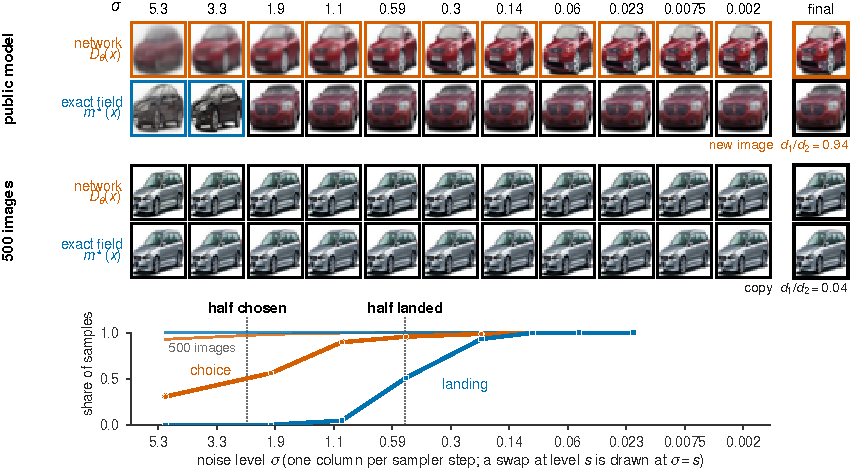
\includegraphics[width=\textwidth]{fig_teaser.pdf}
\caption{One latent, two models (EDM on CIFAR-10). The same Gaussian latent sampled by the public
model, trained on all $50000$ images, none of whose samples copied a training image in our runs
(top), and by a model trained on $500$ images, which copies (middle). In each pair, the first row
is the network's prediction $D_\theta(x)$ of the clean image at the sampler's state $x$, and the
second is the exact field's prediction $m^\star(x)$ from the same state. There is one column per
noise level from $\sigma=5.3$ on; the last column is the output and its nearest training image.
Frames are vermillion (network), blue (exact field) or black where the tile is that training image
(closer to it than a third of its distance to the output's second-nearest one). The exact
prediction settles on the training image at $\sigma=1.9$ for the public model and before
$\sigma=5.3$ for the other: the image is chosen early. The public network's prediction never
reaches it, and the output is a new image ($d_1/d_2=0.94$, with $d_1\le d_2$ the distances to the
two nearest training images). The $500$-image model's prediction is that training image from
$\sigma=5.3$ on, and the output copies it ($d_1/d_2=0.04$). Bottom: the two swaps at level $s$
(Section~\ref{sec:swap}; $500$ latents; public model thick, $500$-image model thin). Choice
(vermillion): share of net$\to$exact endpoints whose nearest training image is the network's own.
Landing (blue): share of exact$\to$net endpoints that end on a training image. Half of the public
model's images are chosen by $s=2.5$, and half of its samples land only from $s=0.51$ (dotted
lines, interpolated in $\log s$). The $500$-image model has chosen $93\%$ of its images at $s=5$
and lands every sample from every swap level.}
\label{fig:intuition}
\end{figure}

\paragraph{Contributions.}
\begin{itemize}\itemsep1pt
\item \emph{A landing condition for learned fields} (Section~\ref{sec:transfer}). A trajectory
  reaches a training example when its error stays a fixed fraction below its distance to that
  example, and does not when the radial ratio approaches one fast enough (Theorem~\ref{thm:relerr}).
  The condition holds at any label and bandwidth, including the class posterior of a
  class-conditional model, and the constant fraction cannot be replaced by one. A trapping
  statement in EDM coordinates and a one-step bound for the deterministic Heun sampler make it
  usable on a finite schedule (Propositions~\ref{prop:trap} and~\ref{prop:heun}).
\item \emph{What the regression loss cannot certify} (Section~\ref{sec:transfer},
  Appendix~\ref{app:transfer}). At an identifying label, a learned endpoint lies within
  $\limsup_{t\uparrow1}(1-t)|\Delta|$ of its training example, where $\Delta$ is the field error
  along the trajectory, and this bound is attained (Lemma~\ref{thm:transfer}). A small regression
  loss does not control this quantity (Proposition~\ref{prop:loss-no-certificate}); an explicit
  risk-transfer condition restores a finite-time bound (Theorem~\ref{thm:risktransfer}). On a
  linear-Gaussian problem, the error met along trajectories exceeds the error on the training law by
  a factor that grows roughly like $(1-t)^{-2}$ (Appendix~\ref{app:measured-transfer}).
\item \emph{The image is chosen early} (Section~\ref{sec:swap}). With the network above the swap
  level and the exact field below it, every endpoint is a training image by construction, so only
  the image is informative. Once the swap is at $\sigma\le1$, that image is the one nearest to the
  network's own sample for at least $88\%$ of samples on every model. Earlier hybrid samplers ran
  the exact field first \citep{bertrand2025closed,liu2025navigation} or exchanged two trained
  networks \citep{dodson2026calm}; to our knowledge, the direction with the network first has not been run before.
\item \emph{Landing is decided late} (Sections~\ref{sec:swap} and~\ref{sec:contraction}). Along the
  sampler's own trajectories, the samples a memorising model copies keep the relative error well
  below one until the last steps, and the others approach one from $\sigma\approx0.14$. The
  contraction that the relative error leaves (the total pull toward the image) over
  $\sigma\in[0.002,0.585]$ has median $1.75$ for copies and $0.68$ for new samples of a
  $2000$-image model; we report it as a description of landing, not as an independent test. The reverse swap, with the exact field first, separates
  memorising from non-memorising models: the $500$-image model lands every sample from every swap
  level, while the public and a $1000$-image model land half of their samples only from $s=0.51$ and
  $s=1.33$. With $36$ or $64$ steps the Heun bound holds at every step for $99.5\%$ of the copies of
  the $500$-image model, and the image reached does not change.
\item \emph{Collapse in trained networks} (Section~\ref{sec:exp1}). Under hard conditioning, trained
  networks from small MLPs to a $35.75$M-parameter U-Net approach the endpoint of the exact field at a
  finite cutoff, late in training.
\end{itemize}
We do not claim a better detector of memorisation. The distance from the denoiser output to the
nearest training image already tells which samples copy at $\sigma\approx1$ (AUC $0.988$ on the
$2000$-image model), at least as well as the late contraction ($0.983$). The theory is conditional.
It names what a measurement of the learned field must show, and it needs the exact field, which only
a party holding the training set can evaluate. The inductive biases of trained denoisers, such as
geometry-adaptive bases \citep{kadkhodaie2024generalization} and locality
\citep{kamb2024creativity,niedoba2024mechanistic}, are candidate forms of the late error that
prevents landing; we do not test them. Proofs are in Appendices~\ref{app:transfer}
and~\ref{app:relerr}.

% ==========================================================================
\section{Related work}
\label{sec:related}

\paragraph{The exact optimum memorises; trained networks depart from it.} The empirical minimiser
of diffusion and flow-matching losses memorises
\citep{pidstrigach2022manifolds,gu2023memorization,biroli2023diffusion,buchanan2025edge,gao2024flow,bertrand2025closed,li2026memory}.
\citet[Theorem~5.3]{wan2025elucidating} show that the flow-matching ODE from a Gaussian source
reproduces its data law exactly, finite training sets included.
\citet[Theorem~6.4]{baptista2025memorization} show that the optimal conditional score only sees the
training examples carrying the queried label. For the exact score of a finite training set,
\citet[Theorem~3.7, version~3]{liu2025pde} prove that almost every deterministic trajectory ends on
a training example. \citet[Theorem~2.5, version~2]{liu2026geometric} prove that when two exact scores
are mixed or guided with a fixed weight, each trajectory converges to one of finitely many
equilibria. Each equilibrium is fixed by its nearest points in the supports, and it need not be a
training example. Companion work \citep{companionA} studies which changes of an exact conditional
field, from label noise and label averaging to guidance and composition, keep its endpoints on the
training set. Here the exact field is only the reference, and the object of study is the learned
field.
Trained denoisers generalise through inductive biases that depart from the exact field
\citep{kadkhodaie2024generalization,kamb2024creativity,niedoba2024mechanistic}.
\citet{bertrand2025closed} show that generalisation in flow matching does not come from the
stochasticity of the regression target. They trace it to the network's failure to fit the
closed-form velocity, which they find around $t\approx0.15$ and near $t=1$, and conclude from a
hybrid sampler that generalisation arises early. Our swaps agree on when the image is chosen, but
show that whether the endpoint is a copy is still open after that (Section~\ref{sec:swap}).

\paragraph{Two times.} For the exact empirical score, \citet{biroli2024dynamical} derive a
speciation time, when the trajectory commits to a class, and a later collapse time, when it falls
into the attractor of one training point, which it then reaches. \citet{raya2023ssb} describe the
first transition as a spontaneous symmetry breaking and observe on trained models that two
individual samples split significantly later than it. \citet{li2024critical} bound, under a perfect score
and for mixtures of strongly log-concave densities, the windows of noise levels in which features
of the sample are decided. Our EDM models are class-conditional, so the first of our two decisions,
which training image the exact field would reach from the network's state, corresponds to the
collapse and not to the speciation. On the public model it is made at or near the noise levels
where the exact posterior over the training images of the class, evaluated at noised test images,
concentrates on one image (Appendix~\ref{app:relerr-exp}, Figure~\ref{fig:posterior}).
\citet{biroli2024dynamical} also measure both times on DDPM U-Nets: the speciation time with $2000$
to $40000$ training images, and the collapse time with $200$ or $2000$, few enough that the networks
reproduce them. In the exact-score picture, landing and
collapse are the same event, because a trajectory that has collapsed reaches its training point.
The public network does not follow this picture: its image is fixed at these noise levels, and it
still does not reach it. \citet{bonnaire2025why} show that memorisation emerges during training on
a time scale that grows with the size of the training set, after a generalisation time that does
not. Our trained networks collapse onto the hard-conditioning endpoint late in training
(Section~\ref{sec:exp1}), and our EDM models memorise at $500$ images and not at $50000$, in line
with that picture. We do not vary the training time systematically
(Section~\ref{sec:limitations}).

\paragraph{Hybrid samplers.} \citet{bertrand2025closed} and \citet{liu2025navigation} run the exact
field first and the trained network afterwards, our exact$\to$net direction. On flow-matching
models of CIFAR-10 and CelebA, \citet{bertrand2025closed} find that a sampler that follows the
closed-form velocity up to $t=\tau$ no longer generalises once $\tau\ge0.3$, by the LPIPS distance
to the nearest training image, and returns almost the closed-form sample from $\tau\ge0.4$.
\citet{liu2025navigation} compute the oracle velocity for latent ImageNet models. They split
sampling into a navigation stage near the prior, where the target blends several training samples,
and a refinement stage dominated by the nearest one. In their mixed sampling, a switch after
$t=0.2$ of their latent-space schedule ($t=0$ at the prior) produces images that closely resemble
training samples, and an earlier one gives novel outputs. They attribute generalisation to navigation and
memorisation to refinement. \citet{dodson2026calm} exchange two trained EDM models of CIFAR-10, one
that copies and one that does not. Exchanging them on $\sigma\in[0.14,8.4]$ moves the share of
copies from $92.2\%$ to $0\%$ and back, and exchanging them above or below this range has little
effect. These works record how close the output ends to a training image.
\citet{cheng2026privacy} run a clipped empirical denoiser through the early steps and a public
network afterwards, to bound the privacy loss of sampling. \citet{briq2026tracing} evaluate the
closed-form velocity at the states of a learned trajectory to attribute samples to clusters of
training images, without a hybrid sampler. Our swaps exchange the network and the exact field in
both directions, at one level $s$ swept along the schedule. We record which training image the
endpoint is nearest to, and whether it is on that image. On the public model the two come apart.
For every swap at $s\le1$ ($t\ge0.5$), the endpoint's nearest training image is that of the field
that ran first for at least $89.6\%$ of samples in either direction. This is close to the time at
which \citet{bertrand2025closed} find the image determined. Yet handed the exact field's state at
$s=1$, the network ends off the training set for $95.6\%$ of samples, and it lands half of them only
when the swap comes at $s=0.5$ ($t=0.67$) (Section~\ref{sec:swap}). Whether a sample copies is thus
decided in what \citet{liu2025navigation} call the refinement stage, by the contraction whose
condition Theorem~\ref{thm:relerr} states.

\paragraph{Late landing.} \citet{li2026kinetic} trace memorisation in flow matching to the terminal
singularity of the empirical optimum, whose velocity grows like $1/(1-t)$, and reduce copying by
damping the velocity late in sampling, a ``soft landing''. In their ablation on $1024$ grayscale
CelebA images, with copies counted by the same distance ratio as here, damping alone for $t\ge0.6$
lowers the share of copies from $37.3\%$ to $30.2\%$ while FID rises from $16.7$ to $35.0$. An early
boost of the velocity alone leaves it at $36.8$--$37.4\%$, and the two together give $31.2\%$ at FID
$14.4$. Theorem~\ref{thm:relerr} states a per-trajectory condition for such landing, and the swaps
indicate where trained networks stop contracting. \citet{favero2025bigger} find that the training
time at which memorisation appears grows in proportion to the size of the training set. They relate
it to the time needed to fit the empirical score at low noise, where the backward process collapses
onto training points.

\paragraph{Where memorisation arises.} For trained diffusion models, other work locates the risk
at medium noise levels \citep{dodson2026calm}, where the relative gap between the denoising errors
on held-out and on training images, a measure of overfitting and not of copying, is also largest
\citep{kaiser2026structural}. \citet{lopezamado2026modes} measure the largest scale at which the
denoiser's fixed-scale dynamics retain an example. Others detect memorisation through basins in
Jacobian spectra, score divergence or the magnitude of the text-conditional guidance term
\citep{jaziri2026spectral,verma2026early,wen2024detecting}, and associative-memory readings
describe the same basins \citep{pham2025memorization}. Changes at medium and high noise levels also
reduce copying. Excluding $\sigma\in[1,5]$ from training lowers it from $78.8\%$ to $0.7\%$ on
$2000$ CIFAR-10 car images \citep{dodson2026calm}. Training the noise levels above a switch level
on noisy images reduces it on small datasets, with Pareto-optimal trade-offs between quality and
copying on $300$ FFHQ images for switch levels $\sigma\in[0.4,4]$ \citep{shah2025ambient}. Under
classifier-free guidance, the prompted prediction of the clean image can already be the training
image at the first denoising step when the pair's training loss is low, for predictions assumed
Bayes-optimal \citep{kim2025how}. Applying guidance only once the trajectory has left an
attraction basin reduces memorisation \citep{jain2025attraction}. These works locate, reduce or
detect memorisation. Theorem~\ref{thm:relerr} and Proposition~\ref{prop:heun} instead give
per-trajectory conditions under which a sampler reaches a training example, and the swaps separate
the choice of the image from the landing on it.

\paragraph{Error bounds.} Small regression error without stability control gives poor endpoint
guarantees \citep[Sec.~3 and Theorem~1]{benton2024error}, and \citet[App.~D, Props.~D.1
and~D.3]{beltran2026reward} construct velocity fields with small $L^2$ error under the interpolant
law whose samples are poor. For interpolants on a finite training set,
\citet[Theorems~4--5]{li2026memory} bound the distance from an Euler-discretised learned endpoint to
the training set from above in terms of the training loss, when the law of the iterates has a
bounded density with respect to the interpolant law. Under non-cancellation and comparability
assumptions, they also
bound its mean-square deviation from the selected training example from below in terms of the
propagated error. Such a density bound implies the risk-transfer condition of
Theorem~\ref{thm:risktransfer}, with $K$ equal to the bound. For the reverse SDE,
\citet[Theorem~2]{pidstrigach2022manifolds} shows that a learned score whose difference from the
empirical score stays bounded still returns only training examples. Lemma~\ref{thm:transfer} and
Proposition~\ref{prop:loss-no-certificate} specialise these considerations to the singular
hard-conditioning target, and Theorem~\ref{thm:relerr} replaces an absolute error bound by a
relative one.

% ==========================================================================
\section{Setting: the exact field of a finite training set}
\label{sec:theory}
% Restated in B's own words (split contract, sec. 3). The mathematical content of the three
% background statements is unchanged; none of them is a contribution of this paper.

This section fixes notation and collects three known facts about the exact minimiser. They are the
reference against which the learned fields of the later sections are measured. Euclidean norms are
written $|\cdot|$, and for a random vector $\Var$ denotes $\tr\Cov$.

\paragraph{Training law and loss.} The training set is $\D=\{(x^i,y^i)\}_{i=1}^N$, with inputs
$x^i\in\R^d$, labels $y^i\in\R^k$, and empirical input law $\rhohat_X=N^{-1}\sum_i\delta_{x^i}$. One
training draw takes an index $I\sim\mathrm{Unif}\{1,\dots,N\}$, a source $X_0\sim\pi_0=\N(0,I_d)$
and a time $t\sim\mathrm{Unif}(0,1)$, all independent. It sets $X_1=x^I$, $Y=y^I$, the linear
interpolant $X_t=(1-t)X_0+tX_1$, and the regression target $U=X_1-X_0$. Label noise of bandwidth
$h>0$ replaces $Y$ by $\widetilde Y=Y+h\omega$ with an independent $\omega\sim\N(0,I_k)$; its kernel
is $K_h(u)=(2\pi h^2)^{-k/2}\exp(-|u|^2/2h^2)$. The flow-matching loss is
\begin{equation}
L_h(v)=\E\big[\,|U-v(X_t,t,\widetilde Y)|^2\,\big],
\label{eq:objective}
\end{equation}
minimised over square-integrable vector fields. At $h=0$ (hard conditioning) $\widetilde Y=Y$, and
the unconditional loss drops the label. For a fixed condition $y$, $p_1^{(h)}(\cdot\mid y)$ denotes
the law at $t=1$ of the minimiser's flow started from~$\pi_0$.

\begin{assumption}[Standing]
\label{as:standing}
\emph{(i)} $\D$ is fixed: the expectation in \eqref{eq:objective} is over
$(I,X_0,t,\omega)$ only. \emph{(ii)} The interpolant is the linear one above.
\emph{(iii)} Labels identify: $y^i\neq y^j$ for $i\neq j$.
\end{assumption}

The linear-Gaussian experiment uses observations $y=Ax+\eta$ with $\eta\sim\N(0,\sigma_{\mathrm{obs}}^2I_k)$.
Its analytic posterior has covariance~$\Sigmapost$, and $\Xhat$ is the covariance of~$\rhohat_X$.

\paragraph{Three facts about the exact field.} With a fixed training set, the minimiser of
\eqref{eq:objective} is a conditional expectation and can be written down. At hard conditioning it
points straight at the training input of the label.

\begin{proposition}[{Exact field at hard conditioning; cf.\ \citealp[Theorem~6.4]{baptista2025memorization}}]
\label{prop:collapse}
Let $h=0$ and fix a training label $y^i$. Then
(a) for $t<1$ the exact field is $v_0^\star(x,t,y^i)=(x^i-x)/(1-t)$ $(\star)$;
(b) the loss reaches $\inf_v L_0(v)=0$;
(c) the flow $\dot x_t=(x^i-x_t)/(1-t)$ is solved by
$x_t=(1-t)x_0+tx^i$, so $x_t\to x^i$ from every $x_0$; and
(d) the endpoint law is $p_1^{(0)}(\cdot\mid y^i)=\delta_{x^i}$, with $\Cov[p_1^{(0)}(\cdot\mid y^i)]=0$.
\end{proposition}
Without the label, the exact flow instead ends on the full empirical law $\rhohat_X$
(cf.\ \citealp{wan2025elucidating}). Both flows return training inputs. The conditional one has
variance $0$ given the label, and the unconditional one has variance $\tr\Xhat$.

With label noise the exact field averages the hard fields of all training examples, with weights
that combine how well each example explains the state and the label.

\begin{proposition}[Exact field under label noise]
\label{prop:kernel-field}
For $h>0$, $t<1$,
\begin{equation}
\vstar(x,t,y)=\sum_i w_i^{(h)}(x,t,y)\,\frac{x^i-x}{1-t},\quad
w_i^{(h)}=\frac{\pi_0\!\big(\tfrac{x-tx^i}{1-t}\big)K_h(y-y^i)}
{\sum_j\pi_0\!\big(\tfrac{x-tx^j}{1-t}\big)K_h(y-y^j)}.
\label{eq:kernel-field}
\end{equation}
\end{proposition}
This is Bayes' rule for the index $I$ given $X_t=x$ and $\widetilde Y=y$, written in the
posterior-mean form of the flow-matching field used by \citet{wan2025elucidating}.

\begin{theorem}[{Exact endpoint law under label noise; cf.\ \citealp{wan2025elucidating}}]
\label{thm:endpoint}
For every $h>0$ and query $y$, with label weights $p_i^{(h)}(y)=K_h(y-y^i)/\sum_jK_h(y-y^j)$,
\begin{equation}
p_1^{(h)}(\cdot\mid y)=\sum_{i=1}^N p_i^{(h)}(y)\,\delta_{x^i}.
\label{eq:endpoint}
\end{equation}
\end{theorem}
At a fixed query $y$, the field \eqref{eq:kernel-field} is the unconditional exact field of the
weighted empirical law on the right of \eqref{eq:endpoint}; \citet[Theorem~5.3]{wan2025elucidating} cover any finite law with positive weights, so this
endpoint law follows from theirs.

\paragraph{The posterior mean and the error of a learned field.} In all three cases the exact field
has the form $\vstar=(m^\star-x)/(1-t)$, where $m^\star=\sum_jw_j^{(h)}x^j$ is the posterior mean
over the training inputs. A learned field that predicts data, $v_\theta=(\hat x_1-x)/(1-t)$,
therefore differs from the exact one by $\Delta$ with $(1-t)\Delta=\hat x_1-m^\star$. The exact
field always returns training inputs. A learned field can end elsewhere only through $\Delta$, and
the next section states which property of $\Delta$ decides it.

% ==========================================================================
\section{When a learned trajectory lands on a training example}
\label{sec:transfer}

A trained network differs from the exact field by an error $\Delta$. This section states which
property of $\Delta$ decides whether a trajectory reaches a training example. The main result,
Theorem~\ref{thm:relerr}, is a relative condition that holds at any label and bandwidth. A
supporting lemma then bounds how far the endpoint can end from its example at an identifying label.
Both statements are about the error along the trajectory, not about the training loss. A field
affine in space can have vanishing hard-conditioned loss and still end with law $\N(a,I_d)$, through
a late amplification (Proposition~\ref{prop:loss-no-certificate}). An explicit risk-transfer
condition restores a finite-time bound (Theorem~\ref{thm:risktransfer}). Both are in
Appendix~\ref{app:teacher-risk}.

\paragraph{The landing condition.} Write $m^\star=\sum_jw_jx^j$ for any posterior mean with
continuous weights $w_j\ge0$, $\sum_jw_j=1$ (at an identifying label or a positive bandwidth, or the
class posterior of Section~\ref{sec:edm}), so that $(1-t)\Delta=\hat x_1-m^\star$ for a field that
predicts data.

\begin{restatable}[Landing under relative field error]{theorem}{thmrelerr}
\label{thm:relerr}
Let $\hat x_1$ be continuous on $\R^d\times[t_1,1)$ and $Z$ a $C^1$ solution of
$\dot Z_t=(\hat x_1(Z_t,t)-Z_t)/(1-t)$ on $[t_1,1)$. Fix an atom $a=x^i$ and write
$n_t=|Z_t-a|$, $e_t=|\hat x_1(Z_t,t)-m^\star(Z_t,t)|$ and
$\zeta_t=(1-w_i(Z_t,t))\max_k|x^k-a|$.
\begin{enumerate}[label=(\alph*),leftmargin=2em]
\item $n$ is locally Lipschitz; where $n_t>0$,
  $(1-t)\dot n_t=\langle\hat e_t,\hat x_1(Z_t,t)-a\rangle-n_t$ with $\hat e_t=(Z_t-a)/n_t$, and
  $(1-t)\dot n_t\le e_t+\zeta_t-n_t$ for almost every $t$.
\item If $e_t\le\bar\varrho\,n_t+\gamma_t$ for a constant $\bar\varrho<1$ and a continuous
  $\gamma\ge0$, and $\gamma_t+\zeta_t\to0$ as $t\uparrow1$, then $Z_t\to a$.
\item If $n_{t_1}>0$ and $\langle\hat e_t,\hat x_1(Z_t,t)-a\rangle\ge(1-\lambda_t)n_t$ whenever
  $n_t>0$, for a continuous $\lambda$ with $\int_{t_1}^1\lambda_t^+/(1-t)\,dt<\infty$, then
  $\inf_tn_t>0$: the trajectory does not reach $a$.
\item The constant $\bar\varrho<1$ in (b) cannot be replaced by $1$.
\end{enumerate}
\proofin{apx:pf-relerr}
\end{restatable}

Part~(b) does not ask for a small error. It asks that the error stay a fixed
fraction below the distance to the example, with $\zeta_t\to0$ once the posterior concentrates on
$a$. This holds on a ball around $a$ at late times (Proposition~\ref{prop:trap}, stated for
uniform or within-class weights; with label-noise priors $\bar\zeta$ carries an extra factor
$\max_{k\ne i}p_k/p_i$). The quantity that decides landing is the radial ratio
$\langle\hat e_t,\hat x_1-a\rangle/n_t$ of~(a). A relative error below one keeps it below one where
$n_t$ is large compared with $\gamma_t+\zeta_t$, and (c) gives a partial converse. Part~(d) shows
that the fraction must be strictly below one.
Appendix~\ref{app:relerr} restates the theorem in EDM's noise coordinates with an explicit trapping
ball (Proposition~\ref{prop:trap}). It also gives the one-step bound for the deterministic Heun
sampler used in practice, whose last steps can extrapolate past the atom
(Proposition~\ref{prop:heun}). Figure~\ref{fig:mechanism} shows the three cases in one dimension.

\begin{figure}[t]
\centering
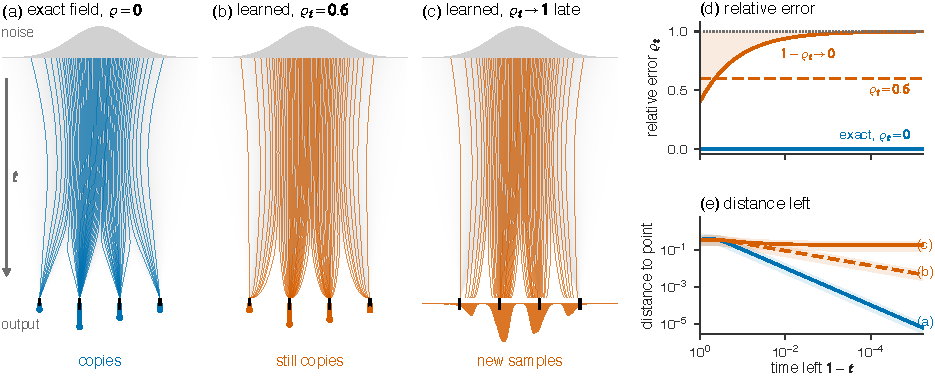
\includegraphics[width=\textwidth]{fig_mechanism.pdf}
\caption{What decides landing, in one dimension. (a--c)~Flows to four training points (black
ticks) from $1500$ sources ($64$ drawn) over the exact density $p_t$ (grey), with the source law on
top and the output at the bottom: a stem is a point mass on a training point, with height equal to
its probability; a shaded curve is a density. (a)~The exact field, $\hat x_1=m^\star$, returns the
training points with the label-noise weights $0.12$, $0.48$, $0.28$, $0.12$
(Theorem~\ref{thm:endpoint}). (b)~A learned field $\hat x_1=m^\star+\varrho_t(Z-m^\star)$ with
$\varrho_t=0.6$ still copies. (c)~With $1-\varrho_t=0.6(1-t)^{1/2}$, whose integral against
$dt/(1-t)$ is finite, the trajectories stop short of the training points: new samples. (d)~The
relative error of the three fields; shaded, the contraction $1-\varrho_t$ left to field (c).
(e)~Median distance (interquartile range shaded) to the nearest training point at the end: it falls
like $1-t$ in (a) and like $(1-t)^{0.4}$ in (b), and tends to a positive limit in (c), as in
Theorem~\ref{thm:relerr}(b) and~(c).}
\label{fig:mechanism}
\end{figure}

\paragraph{The size of the miss at an identifying label.} Theorem~\ref{thm:relerr} says whether a
trajectory lands. When the label identifies one training example, the next lemma also bounds how far
from it the endpoint can end.

% Demoted from theorem to lemma (split contract, sec. 2 and 5); statement unchanged.
\begin{restatable}[Endpoint transfer at an identifying label]{lemma}{thmtransfer}
\label{thm:transfer}
Fix an identifying label with atom $a=x^i$. Let $Z$ be absolutely continuous on $[0,1)$ with
$Z_0=x_0$ and
\[
\dot Z_t=\frac{a-Z_t}{1-t}+\Delta(Z_t,t)\quad\text{for almost every }t,
\]
where $s\mapsto\Delta(Z_s,s)$ is integrable on every $[0,T]$ with $T<1$. Then for $t<1$
\begin{equation}
Z_t-a=(1-t)(x_0-a)+(1-t)\int_0^t\frac{\Delta(Z_s,s)}{1-s}\,ds,
\qquad
\limsup_{t\uparrow1}|Z_t-a|\le\limsup_{t\uparrow1}\,(1-t)|\Delta(Z_t,t)|.
\label{eq:transfer}
\end{equation}
The bound is attained: for $\Delta(x,t)=c/(1-t)$ both sides equal $|c|$ from every $x_0$. If
the field predicts data, $v_\theta(x,t)=(\hat x_1(x,t)-x)/(1-t)$, then
$\limsup_{t\uparrow1}|Z_t-a|\le\limsup_{t\uparrow1}|\hat x_1(Z_t,t)-a|$.
\proofin{apx:pf-transfer}
\end{restatable}

The argument is elementary. What it adds is the reading: a learned trajectory stays away from its
atom only if the scaled error $(1-t)|\Delta|$, equivalently the error of the implied endpoint
prediction, stays away from zero up to $t=1$. Errors of order $o((1-t)^{-1})$ still collapse. The
bound is informative when the scaled error is controlled independently of the endpoint, for
instance by an estimate of the learned field. It is not a separate test of the endpoint. Since
$(1-t)\Delta(Z_t,t)=(1-t)v_\theta(Z_t,t)+Z_t-a$, if $v_\theta$ stays bounded along a trajectory with
$Z_t\to z$, then $(1-t)\Delta(Z_t,t)\to z-a$ and the bound holds with equality. A correlation
between the two measured quantities would therefore carry little additional information. At
positive bandwidth the same holds near an atom, once the trajectory enters a small ball with a
small scaled error there.

\begin{restatable}[Local transfer at positive bandwidth]{proposition}{proplocaltransfer}
\label{prop:localtransfer}
Let $h>0$, fix $y$, write $v^\star=\vstar(\cdot,\cdot,y)$, and let $a=x^i$ be an atom with
$\ell =\min_{j\ne i}|x^j-a|$ and $r\in(0,\ell /2)$. There is $t_\star<1$, depending only on the
atoms, $p^{(h)}(y)$ and $r$, with the following property. Let $v^\star+\Delta$ be locally
Lipschitz on $\R^d\times[0,1)$, let $t_0\in[t_\star,1)$, and let $Z$ be the maximal solution of
$\dot Z=v^\star(Z,t)+\Delta(Z,t)$ from a point $Z_{t_0}$. If $|Z_{t_0}-a|<r/4$ and
$(1-t)|\Delta(x,t)|\le r/4$ whenever $|x-a|\le r$ and $t_0\le t<1$, then $|Z_t-a|<r$ for
all $t\in[t_0,1)$ and $\limsup_{t\uparrow1}|Z_t-a|\le\limsup_{t\uparrow1}(1-t)|\Delta(Z_t,t)|$.
\proofin{apx:pf-localtransfer}
\end{restatable}

\paragraph{What the statements do and do not say.} Theorem~\ref{thm:relerr},
Lemma~\ref{thm:transfer} and Proposition~\ref{prop:localtransfer} are conditional. They do not infer
the error along trajectories from the training loss, and they do not assert that a trained network
enters the ball. They name what a measurement would need to show.
Appendix~\ref{app:measured-transfer} measures the trajectory error on the linear-Gaussian problem
and on retrained CIFAR-10 U-Nets, and Section~\ref{sec:edm} measures the relative error on EDM
models. Whether a learned field can end exactly on an atom depends on how its regularity degenerates
at $t=1$. If the spatial Lipschitz constant of a velocity network and $|v_\theta(0,t)|$ are both
integrable up to $t=1$, its flow map is bi-Lipschitz by Gr\"onwall's inequality, and it carries the
Gaussian source to a law without atoms \citep{companionA}. The collapse of such a network in
Section~\ref{sec:exp1} is therefore an approach to the atom at a finite cutoff, not the atom
itself.
% companionA kept for the no-atom statement (Proposition "regular" of paper A); the Gronwall
% sentence keeps B readable without it.

% ==========================================================================
\section{Experiments}
\label{sec:experiments}

The experiments ask two questions. First, do trained networks approach the exact endpoint when the
target is the singular hard-conditioning field (Section~\ref{sec:exp1})? Second, on image models
that do and do not copy, when is the training image chosen and when is landing on it decided
(Sections~\ref{sec:edm}--\ref{sec:contraction})? The first part uses small synthetic problems and a
CIFAR-10 inpainting U-Net; the second uses class-conditional EDM models of CIFAR-10, where the
exact field can be evaluated and swapped in for the network.

\paragraph{Setup.} The linear-Gaussian problem (EXP-1) has $d{=}2$, $k{=}1$, $N{=}200$,
$\sigma_{\mathrm{obs}}{=}0.1$, a 4-layer width-128 MLP trained with Adam without early stopping,
RK4 integration to $t{=}1{-}10^{-3}$, and $M{=}1000$ samples at 20 training and 8 held-out
conditions; five seeds, each fixing both the instance and the training randomness. A bracket
after a mean is a $95\%$ Student-$t$ interval over the seeds (four degrees of freedom), and $\pm$
a population standard deviation. Appendix~\ref{app:expdetails} gives all settings.

\subsection{Collapse in trained networks}
\label{sec:exp1}

\begin{figure}[t]
\centering
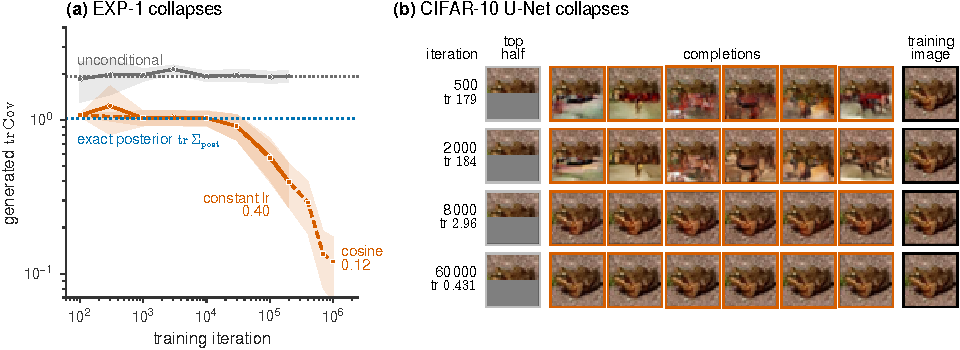
\includegraphics[width=\textwidth]{fig_collapse.pdf}
\caption{Collapse in trained networks at hard conditioning. (a)~EXP-1 at $h=0$, five seeds (mean
$\pm$ one population standard deviation). The generated variance stays at $\tr\Sigmapost$ of the
exact posterior up to about $10^4$ iterations and then falls, to $0.40$ at $2\times10^5$ with a
constant learning rate (solid) and $0.12$ at $10^6$ with a cosine schedule (dashed), while the
unconditional model (grey) keeps $\tr\Xhat$. (b)~The $35.75$M-parameter CIFAR-10 U-Net at $h=0$,
first instance: the observed top half, six completions of one condition from different sources
$x_0$ and the training image at four checkpoints, with the generated trace (training-time
estimator, $8$ conditions, $M=16$). From iteration $8000$ the completions coincide with the
training image. Figure~\ref{fig:collapse-details} shows the other EXP-1 and CIFAR-10 diagnostics.}
\label{fig:collapse}
\end{figure}

\paragraph{Hard conditioning.} \emph{Collapse} of a trained network here means finite-cutoff
collapse: the variance falls toward zero at the cutoff. It is not an endpoint atom, which a
velocity MLP lacks (Section~\ref{sec:transfer}). On EXP-1 the conditional variance tracks the
posterior, $\tr\Sigmapost=1.018$, up to $\sim\!10^4$ iterations, then collapses: $0.396$
$[0.220,0.573]$ at $2\times10^5$ and $0.120$ $[0.046,0.195]$ at $10^6$ with a cosine schedule. In
the same period the velocity approaches $(\star)$ and the generated mean moves to $x^i$
(Figures~\ref{fig:collapse}a and~\ref{fig:collapse-details}, Table~\ref{tab:exp1}). On average the distances of the generated
mean to the training atom and to the posterior mean cross between $10^5$ and $2\times10^5$
iterations; their paired difference is $-0.28$ $[-0.57,0.01]$ at $2\times10^5$, where one seed of
five has not crossed, and $-0.68$ $[-0.94,-0.42]$ at $10^6$. The unconditional baseline keeps
$\tr\Cov=1.926$ $[1.690,2.163]$ against $\tr\Xhat=1.931$ (paired ratio $0.997$ $[0.971,1.024]$), as
the exact unconditional field predicts. The memorisation ratio of \citet{yoon2023memorization}
reaches $0.650$ $[0.604,0.696]$ conditionally and $0.389$ $[0.345,0.433]$ unconditionally. A
bimodal mixture posterior (EXP-2) and MNIST inpainting (EXP-3) show the same collapse. It occurs
for every architecture and optimiser we tried, and the spread across seeds is mostly due to the
problem instance (Appendix~\ref{app:exp}).

\label{sec:cifarddpm}
\paragraph{At realistic capacity.} A standard DDPM U-Net ($35.75$M parameters) trained on
CIFAR-10 bottom-half inpainting ($N{=}2000$, $d{=}3072$, $k{=}1536$, $60000$ iterations) collapses
at $h{=}0$. The conditional trace falls from $179.1$ at iteration $500$ to $0.431$ (training-time
estimator; $0.458$ re-measured at $M=256$, Appendix~\ref{app:exp4}), and the
generated mean identifies the correct training image at $48/48$ conditions, in this run and in
networks retrained on each of three independently redrawn instances. The three instances follow the
same trajectory, and in the displayed conditions the completions coincide with the training image
from iteration $8000$ (Figure~\ref{fig:collapse}b; Figure~\ref{fig:cifar-training-grid} shows all
checkpoints).

\paragraph{Measured transfer.} On EXP-1 the error met along learned trajectories exceeds the
error on the training law by a factor of $127\pm40$ at $1-t=0.1$ and $(2.0\pm2.2)\times10^7$ at
$10^{-4}$, so the regression loss does not bound the endpoint (Appendix~\ref{app:measured-transfer}).
On CIFAR-10 U-Nets retrained with label noise of bandwidth $h=4$ and $h=6$, refining the integrator
and the cutoff barely changes the off-atom fraction (the share of new images, not copies), while the exact field has none. The off-atom
samples are those with large scaled error along their own trajectories, with
AUC $0.97$ and $0.95$ at $h=4$ and $6$ by
$t\approx0.53$ and $0.99$ and $0.98$ by $t\approx0.63$. The same network along the exact
trajectory from the same source separates them weakly if at all (AUC at most $0.58$ from
$t\approx0.63$ on).

\FloatBarrier

\subsection{Landing in EDM image models}
\label{sec:edm}

This section and the next two measure the landing condition on class-conditional EDM denoisers
of CIFAR-10 \citep{karras2022elucidating}. We use the public model trained on all $50000$ images,
and three models with the same architecture trained here for $10$\,Mimg without augmentation on
class-balanced subsets, two of $500$ images (different subsets and seeds) and one of $2000$. The
exact field $m^\star$ is the posterior mean over the training images of the class $c$. The class
label is not identifying, so Lemma~\ref{thm:transfer} does not apply, while the relative condition
does. We measure it in EDM's own coordinates, that is, through Proposition~\ref{prop:trap}, the form
that Theorem~\ref{thm:relerr} takes there. Along the EDM state $x$ we record three quantities: the
distance $n=|x-a|$ to a training image $a$, the error $e=|D_\theta-m^\star|$, and the relative error
$\varrho=e/n$. The radial identity reads $\sigma\,dn/d\sigma=n-\langle\hat e,D_\theta-a\rangle$, as in
the proof of Proposition~\ref{prop:trap}. The contraction that $\varrho$ leaves over a range of
levels is $\int(1-\varrho)\,d\log(1/\sigma)$. These are not the quantities of
Theorem~\ref{thm:relerr} in the coordinates $t=1/(1+\sigma)$ and $Z=tx$, where $n_t=|tx-a|$; we did
not record those. All samples use EDM's deterministic $18$-step Heun sampler. A sample is on-atom (a copy) when its
distance to the nearest training image of its class is less than $1/3$ of that to the second
nearest, and off-atom (a new image) otherwise, as in Appendix~\ref{app:measured-transfer}. The
$500$-image models memorise: $41$ of $1000$ samples
($4.1\%$) are off-atom, and $4.4\%$ for the second subset. The $2000$-image model is balanced, with
$50.1\%$ off-atom, and the public model has only off-atom samples. The exact field has none. The
swap experiments also use a model trained on a class-balanced subset of $1000$ images and stopped
after $0.5$\,Mimg, which has only off-atom samples. Unless stated otherwise, numbers below are for
the first $500$-image model; the second gives the same conclusions (Appendix~\ref{app:relerr-exp}).

\subsection{Choose early, land late: swapping the field mid-trajectory}
\label{sec:swap}

Because the exact field can be evaluated on these models, we can separate the choice of the image
from the landing on it by intervention, not only by correlation. From the same Gaussian latents we
run the Heun sampler with two hybrid denoisers. \emph{Net$\to$exact} uses $D_\theta$ at the noise
levels of the schedule above $s$ and the exact posterior mean $m^\star$ at those $\le s$.
\emph{Exact$\to$net} does the reverse, the direction of the hybrid samplers of
\citet{bertrand2025closed} and \citet{liu2025navigation}. The two directions answer different
questions. Net$\to$exact ends on a training image by construction, so it tells only which image the
network's state had chosen at the swap level. Exact$\to$net tells whether a given network lands from
the state the exact field hands it. It is uninformative on a memorising model, which lands from
every state, so we use it to tell memorising from non-memorising models. For each swap we record
whether the endpoint is off-atom, and whether its nearest training image equals that of the learned
endpoint (\emph{$=$L}, the network's own sample) or of the exact endpoint (\emph{$=$E}). The swap
levels are $s\in\{5,2,1,0.5,0.2,0.1,0.05,0.02\}$, that is $t=1/(1+s)$ from $0.17$ to $0.98$. We use
$500$ samples ($50$ per class) of three models: the public model and the $1000$-image model, both
with all samples off-atom, and the first $500$-image model, with $3.8\%$ off-atom on these latents
(Figure~\ref{fig:swap}, Table~\ref{tab:swap}). The learned and exact endpoints share their nearest
image for $13.8\%$, $21.0\%$ and $35.4\%$ of samples on the three models.

\begin{figure}[t]
\centering
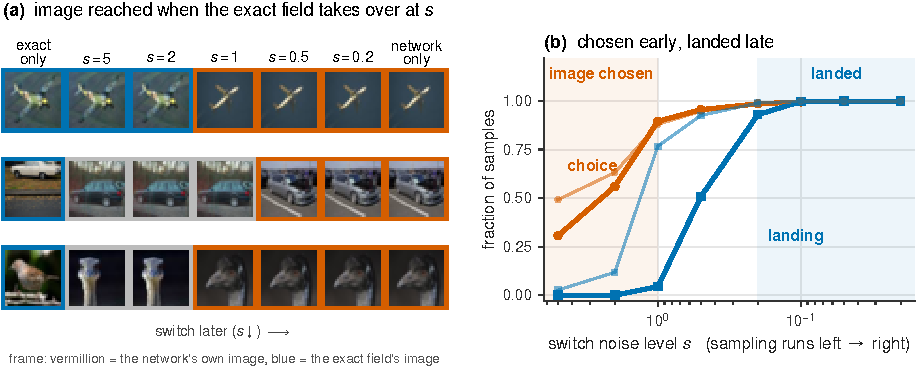
\includegraphics[width=\textwidth]{fig_swap.pdf}
\caption{The trained sampler chooses its image early and lands late (EDM on CIFAR-10).
(a) Public model; each row is one latent. Each tile is the training image on which
net$\to$exact ends (network for $\sigma>s$, exact field for $\sigma\le s$) when the switch is at
$s$, from the exact field alone (left) to the network alone (right). Frames: vermillion, the
network's image; blue, the exact field's image; grey, neither. Each row is the first latent of its
class whose two images differ and whose image changes to the network's between $s=5$ and $s=0.2$;
over all $500$ latents, a switch at $s=1$ already ends on the network's image for $89.6\%$
(Table~\ref{tab:swap}). (b) Choice: share of net$\to$exact endpoints whose nearest training image is
the network's ($=$L). Landing: share of exact$\to$net endpoints (exact field for $\sigma>s$, network
for $\sigma\le s$) that end on a training image ($1-$off). Shaded: $s\ge1$, over which the image is
chosen, and $s\le0.2$, from which at least $93\%$ of the public model's samples land. Thick lines:
public model; thin: $1000$-image model; $500$ latents each. Net$\to$exact ends on a training image
at every $s$ by construction, since the last step returns the exact field's output; only the image
it ends on is informative.}
\label{fig:swap}
\end{figure}

\begin{table}[t]
\centering\small
\resizebox{\textwidth}{!}{%
\begin{tabular}{@{}rr ccc ccc ccc@{}}
\toprule
& & \multicolumn{3}{c}{public ($50000$ images)} & \multicolumn{3}{c}{$1000$ images, $0.5$\,Mimg} & \multicolumn{3}{c}{$500$ images}\\
\cmidrule(lr){3-5}\cmidrule(lr){6-8}\cmidrule(l){9-11}
& & net$\to$exact & \multicolumn{2}{c}{exact$\to$net} & net$\to$exact & \multicolumn{2}{c}{exact$\to$net} & net$\to$exact & \multicolumn{2}{c}{exact$\to$net}\\
$s$ & $t$ & $=$L & off & $=$E & $=$L & off & $=$E & $=$L & off & $=$E\\
\midrule
$5$    & $0.17$ & $0.306$ & $1.000$ & $0.422$ & $0.492$ & $0.974$ & $0.784$ & $0.928$ & $0.000$ & $0.954$\\
$2$    & $0.33$ & $0.560$ & $1.000$ & $0.832$ & $0.632$ & $0.882$ & $0.976$ & $0.982$ & $0.000$ & $0.996$\\
$1$    & $0.50$ & $0.896$ & $0.956$ & $1.000$ & $0.880$ & $0.232$ & $1.000$ & $0.996$ & $0.000$ & $1.000$\\
$0.5$  & $0.67$ & $0.956$ & $0.492$ & $1.000$ & $0.948$ & $0.074$ & $1.000$ & $0.998$ & $0.000$ & $1.000$\\
$0.2$  & $0.83$ & $0.986$ & $0.070$ & $1.000$ & $0.982$ & $0.010$ & $1.000$ & $1.000$ & $0.000$ & $1.000$\\
$0.1$  & $0.91$ & $0.996$ & $0.002$ & $1.000$ & $1.000$ & $0.000$ & $1.000$ & $1.000$ & $0.000$ & $1.000$\\
$0.05$ & $0.95$ & $0.998$ & $0.000$ & $1.000$ & $1.000$ & $0.000$ & $1.000$ & $1.000$ & $0.000$ & $1.000$\\
$0.02$ & $0.98$ & $1.000$ & $0.000$ & $1.000$ & $1.000$ & $0.000$ & $1.000$ & $1.000$ & $0.000$ & $1.000$\\
\midrule
\multicolumn{2}{@{}l}{no swap: off-atom} & \multicolumn{3}{c}{learned $1.000$, exact $0.000$} & \multicolumn{3}{c}{learned $1.000$, exact $0.000$} & \multicolumn{3}{c}{learned $0.038$, exact $0.000$}\\
\bottomrule
\end{tabular}}
\caption{Denoiser swap at level $s$, $500$ samples per model. ``off'': fraction off-atom;
$=$L, $=$E: fraction whose nearest training image is that of the learned, resp.\ exact, endpoint.
net$\to$exact is off-atom for no sample at any $s$ on any model by construction: the sampler's last
step returns the exact field's output at $\sigma=0.002$, the nearest training image of the class,
and every endpoint lies within $10^{-5}$ of it.}
\label{tab:swap}
\end{table}

\paragraph{The image is chosen early.} With the network running down to $s$ and the exact field
below, every sample of every model ends on a training image, at every $s$. This holds by
construction rather than as a finding. The sampler's last step is an Euler step from
$\sigma=0.002$ to $0$, which returns the denoiser output at $\sigma=0.002$. For the exact field that
output is the nearest training image of the class to double precision, from any state that
is not almost exactly equidistant from two of them. The exact field used only for the last of the
$35$ denoiser evaluations of the $18$-step sampler would already end every sample on a training
image. What this direction measures is which image is reached. The image reached is the one nearest
to the network's own endpoint in $31$, $56$, $90$, $99$ and $100\%$ of samples for $s=5,2,1,0.2,0.02$ on the
public model, in $49$, $63$, $88$, $98$ and $100\%$ on the $1000$-image model, and in $92.8$, $98.2$ and
$99.6\%$ for $s=5,2,1$ and all samples from $s\le0.2$ on the $500$-image model. Interpolated in
$\log s$ between swap levels, this share passes $50\%$ at $s=2.48$ and $90\%$ at $s=0.95$ on the
public model ($95\%$ bootstrap intervals $[2.13,2.87]$ and $[0.74,1.05]$). On the public and the $1000$-image model the learned endpoint is almost equidistant from its two
nearest training images (median $d_1/d_2$ $0.977$ and $0.949$). So $=$L does not mean that the
network's sample comes close to a training image. It means that the network's state at the switch
already lies in the exact field's basin of the image nearest to that sample. The basin is decided by
the network's trajectory, not by the latent: among the $431$ public-model samples whose learned and
exact images differ, a switch at $s=1$ ends on the network's image for $379$ ($87.9\%$) and on the
exact field's for $11$ ($2.6\%$). The other direction gives the same time from the other side. Once
the exact field has run down to $\sigma=1$, the network no longer changes which image is nearest to
the endpoint ($=$E is $1.000$ for $s\le1$ on all three models), while from $s=5$ it re-selects for
$58\%$ of samples on the public model, $22\%$ on the $1000$-image model and $5\%$ on the $500$-image
model. The image is therefore selected by $\sigma\approx1$, in the medium-noise band where
\citet{dodson2026calm} locate memorisation risk, and earlier on the memorising model, which selects
$93\%$ of its images by $\sigma=5$. The swaps of \citet{dodson2026calm} between two trained networks
exchange the range $\sigma\in[0.14,8.4]$ as a whole (Section~\ref{sec:related}). That range contains
both of the decisions that the swap level $s$ separates here.

\paragraph{The reverse swap separates memorising from non-memorising models.} The exact field ends on
a training image from whatever state it is handed, so evidence on landing has to come from this
direction, where the network runs last. Only the memorising network lands from every
swap level; the two networks that do not memorise land only from late levels. With the exact
field down to $s$ and the network below, the public model ends off-atom for $100\%$ of samples at $s\ge2$, $95.6\%$ at
$s=1$, $49.2\%$ at $s=0.5$, $7.0\%$ at $s=0.2$ and $0.2\%$ at $s=0.1$; the $1000$-image model for
$97.4\%$ at $s=5$, $23.2\%$ at $s=1$ and none from $s\le0.1$. Interpolated in $\log s$, half of
the samples land from $s=0.51$ ($95\%$ interval $[0.47,0.54]$) on the public model and from
$s=1.33$ ($[1.29,1.37]$) on the $1000$-image model, later than half of the images are chosen
($s=2.48$ and $4.74$). At $90\%$ the order is the same ($0.95$ against $0.21$, and $0.82$ against
$0.56$). For $s\le1$ the samples that end off-atom miss the image that the exact field's state had
fixed: their nearest image is still the exact one. When the switch is late enough to end on-atom,
this is partly because little time is left. From $s=0.1$ to $0.02$ the median endpoint distance
to the nearest image falls roughly in proportion to $s$: $2.57$, $1.37$ and $0.61$ on the public
model ($2.63$, $1.47$, $0.68$ on the $1000$-image model; log--log slopes $0.90$ and $0.84$,
against $0.47$ from $s=5$ to $0.5$ on the public model). The exact field would end at
distance $0$. The network does contract, but weakly. Suppose the state at the last level $\sigma$ of
the exact field lies at the distance $\sigma\sqrt d$ from the image that an exact trajectory has
there (the hand-over distance was not recorded). Then the remaining steps of these late swaps on
the public model shorten it by a factor of about $2$ to $3$, or of about $1.4$ to $2.2$ if the
exact field is credited with its half of the mixed Heun step at the hand-over. This is close to
the boundary case of Theorem~\ref{thm:relerr}(d), a relative error near one that neither contracts
nor expands. This also matches the relative error of the public model along its own trajectories, $0.925$
at $\sigma=0.14$ and $0.997$ at $\sigma=0.023$ (Table~\ref{tab:edm-rho}).

The memorising $500$-image model behaves the other way. Handed the exact state at any $s$, its late
field ends on-atom for every sample, on the exact field's image ($=$E at least $0.954$) rather than
on its own ($=$L between $0.354$ and $0.374$, the agreement without a swap). Its late field thus
contracts toward whichever training image the state is near, not toward the image it selected. Its
median endpoint distance falls from $1.67$ at $s=5$ to $0.45$ at $s=0.02$, on-atom by the relative
criterion but not at distance $0$. The $19$ samples that this model leaves off-atom when it runs
alone all land under exact$\to$net at every swap level, even $s=5$. From the exact field's state
the same late field lands them, so their failure to land is set by the state the network reaches
above $\sigma=5$.

\paragraph{A window of exact field.} On the public model we also used the exact field only on a
window of levels $\sigma\in(\sigma_{\rm lo},\sigma_{\rm hi}]$, with the network above and below
it, from the same $500$ latents (Table~\ref{tab:window}). Two predictions were written down before
the run. The first was that with the exact field down to $\sigma_{\rm lo}$ the median endpoint
distance $d_1$ is proportional to $\sigma_{\rm lo}$, with $d_1/\sigma_{\rm lo}$ between $20$ and
$35$. This restated the exact$\to$net runs above, which the windows $(\sigma_{\rm lo},\infty)$ repeat
on the same latents and reproduce sample by sample, so it is not an independent test. The ratio is
in that range for $\sigma_{\rm lo}\le0.2$ ($30.3$, $27.5$, $25.7$ and $21.1$ at
$\sigma_{\rm lo}=0.02$, $0.05$, $0.1$ and $0.2$) but not at $0.5$ and $1$ ($12.9$ and $9.2$), so
by its own criterion it fails. The second, and the only new test, was that for
$\sigma_{\rm hi}\ge0.5$ the median $d_1$ depends only on $\sigma_{\rm lo}$, where the network takes
over again. It is refuted. With $\sigma_{\rm lo}=0.1$ the median is $4.16$ for the window $(0.1,0.5]$
and $2.48$ for $(0.1,2]$, a ratio of $0.60$ ($[0.58,0.61]$), and $(0.1,0.5]$ leaves $21\%$ of the
samples off-atom ($[18,25]\%$), against $0.2\%$ when the exact field runs from the start down to
$0.1$. Which image is reached is set by the window's upper end: the share on the network's own
image equals that of net$\to$exact at $s=\sigma_{\rm hi}$ ($0.956$, $0.896$, $0.560$ and $0.306$ for
$\sigma_{\rm hi}=0.5$, $1$, $2$ and $5$), and the image itself agrees for at least $99.6\%$ of
samples. A window that starts at $\sigma_{\rm hi}\le1$ ends farther from the image than the exact
field run from the start down to the same $\sigma_{\rm lo}$. Only windows that start at
$\sigma_{\rm hi}\ge2$ give a final distance that depends on $\sigma_{\rm lo}$ alone ($1.33$, $1.33$
and $1.37$ for $(0.05,2]$, $(0.05,5]$ and $(0.05,\infty)$). With the same network below
$\sigma_{\rm lo}$, landing thus depends on the state it is handed, not on the late field alone.

\paragraph{Reading.} The image is decided at medium noise, by the network for its own samples and
by whichever field runs there in the swaps. Whether the endpoint is that image is decided by the
field that runs below the switch, from the state it is handed. From the exact
field's state at $s=2$ the memorising network lands every sample, the $1000$-image model $12\%$
and the public model none. From $s=1$ the $1000$-image model lands $77\%$ and the public model
$4\%$, although the $1000$-image model lands none of its own samples. The swap levels over which
exact$\to$net goes from almost no to almost all samples on-atom, $s=2$ to $0.1$ on the public model
and $s=5$ to $0.2$ on the $1000$-image model, indicate where the network's late field stops
contracting. These swaps are interventions on one latent seed, one
deterministic sampler and the noise levels of the $18$-step schedule. The $1000$-image model is
likely undertrained. In addition, the off-atom criterion is relative, so ``on-atom'' at small $s$ does not
mean exact landing. The next section measures the contraction along the network's own
trajectories, and Section~\ref{sec:limitations} lists the intervention that would turn it into a
prediction.

\FloatBarrier

\subsection{The relative error along the sampler's own trajectories}
\label{sec:contraction}

The swaps show where landing is decided; this section describes how. We measure the relative error
$\varrho$ and the contraction it leaves along the unmodified sampler, and compare copies with new
samples. These measurements describe the mechanism of Theorem~\ref{thm:relerr} on trained
networks. They are not an independent test of it: part of the separation near the end is
bookkeeping, and the bound of Proposition~\ref{prop:heun} holds by construction when $\varrho$ is
measured along the trajectory.

\begin{figure}[t]
\centering
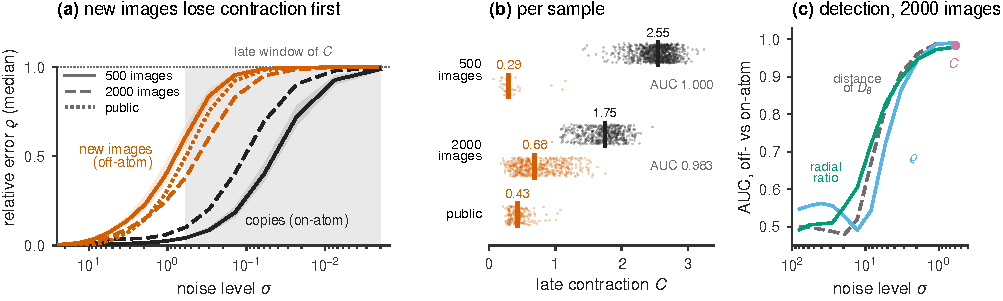
\includegraphics[width=\textwidth]{fig_landing.pdf}
\caption{Relative error and late contraction along the sampler's trajectories (EDM on CIFAR-10;
$1000$ samples per trained model, $200$ for the public model). (a)~Median relative error
$\varrho=e/n$, with $n$ the distance to the endpoint's nearest training image as in
Table~\ref{tab:edm-rho}, for samples that copy a training image (on-atom, black) and for new images
(off-atom, vermillion): $500$-image model (solid, interquartile range shaded), $2000$-image model
(dashed), public model (dotted; all its samples are off-atom). On the $500$-image model the
off-atom median passes $0.9$ by $\sigma=0.14$, the on-atom median only by $\sigma=0.0075$.
(b)~Per sample, the late contraction $C=\int(1-\varrho)\,d\log(1/\sigma)$ over
$\sigma\in[0.002,0.585]$ (grey window in (a)), with the medians and the AUC of $C$ for telling off-
from on-atom samples. (c)~On the balanced $2000$-image model, the AUC at each $\sigma\ge0.585$ of
$\varrho$ and of the radial ratio of Proposition~\ref{prop:trap} (the EDM form of
Theorem~\ref{thm:relerr}(a)), both anchored at the nearest training image of $D_\theta(x,\sigma)$ so
that they use nothing after $\sigma$, and of the distance from $D_\theta$ to that image (dashed).
The late contraction of (b), whose window starts at $\sigma=0.585$, gives $0.983$ with either
anchor, against $0.990$ for that distance at $\sigma=0.585$.}
\label{fig:landing}
\end{figure}

\begin{table}[t]
\centering\small
\begin{tabular}{@{}lccccc@{}}
\toprule
$\sigma$ & $1.92$ & $0.585$ & $0.140$ & $0.023$ & $0.002$\\
\midrule
$\varrho$, subset model, on-atom & $0.015$ & $0.043$ & $0.185$ & $0.725$ & $0.988$\\
$\varrho$, subset model, off-atom & $0.231$ & $0.613$ & $0.957$ & $0.998$ & $1.000$\\
$\varrho$, public model & $0.146$ & $0.499$ & $0.925$ & $0.997$ & $1.000$\\
AUC of $\varrho$, subset model & $0.999$ & $1.000$ & $1.000$ & $1.000$ & $0.995$\\
\midrule
$\varrho$, $2000$ images, on-atom & $0.041$ & $0.103$ & $0.405$ & $0.906$ & $0.997$\\
$\varrho$, $2000$ images, off-atom & $0.151$ & $0.384$ & $0.832$ & $0.989$ & $1.000$\\
AUC of $\varrho$, $2000$ images & $0.946$ & $0.990$ & $0.983$ & $0.970$ & $0.929$\\
\bottomrule
\end{tabular}
\caption{Median relative field error $\varrho_t=e_t/n_t$ along EDM trajectories, with $n_t=|x-a|$
the distance from the state $x$ to the endpoint's nearest training image $a$; AUC is the probability that an off-atom
sample has the larger $\varrho$. Top: the first $500$-image model ($41$ off-atom samples) and the
public model; bottom: the balanced $2000$-image model ($501$ off-atom of $1000$). Anchoring at the
nearest training image of $D_\theta(x,\sigma)$ instead, which uses no information after $\sigma$,
gives the same AUC at every $\sigma$ (Appendix~\ref{app:relerr-exp}).}
\label{tab:edm-rho}
\end{table}

\paragraph{Relative error and late contraction.} On the $500$-image model the groups are far
apart. On-atom samples keep $\varrho_t$ well below one until the last steps, while off-atom samples
and the samples of the public model approach $\varrho_t=1$ from $\sigma\approx0.14$ on
(Table~\ref{tab:edm-rho}, Figure~\ref{fig:landing}a). On a finite schedule this does not make the
hypothesis of Theorem~\ref{thm:relerr}(b) fail, since $34$ of the $41$ off-atom samples, and $195$
of the $200$ samples of the public model, keep $\varrho_t<1$ at every level from $\sigma=0.585$ to
$0.002$. The approach to one instead leaves little of the contraction that~(b) uses, which we
measure below. This is consistent with, but does not verify, the hypothesis of~(c), which concerns
the radial ratio and is an asymptotic condition that a finite schedule cannot check. Near the end
the anchor and the off-atom label are both set by the endpoint, so the separation there is partly
bookkeeping. The informative range is earlier, where the predictive anchor of
Appendix~\ref{app:relerr-exp} gives the same AUC. On the balanced $2000$-image model the contrast is one of degree: almost every sample of either
group has $\varrho_t<1$ at every step, and the on-atom median also approaches one at the last step.
What Theorem~\ref{thm:relerr}(b) uses is the contraction that the relative error leaves,
$\int(1-\varrho_t)\,d\log(1/\sigma)$. Over the late noise levels $\sigma\in[0.002,0.585]$ it is $1.75$
for on-atom against $0.68$ for off-atom samples (medians, AUC $0.983$, interval $[0.977,0.988]$),
and $2.55$ against $0.29$ (AUC $1.000$) on the $500$-image model. The radial identity of
Proposition~\ref{prop:trap}, the EDM form of Theorem~\ref{thm:relerr}(a), holds for the flow, and
the discrete sampler follows it. Over the same window, the decrease of $\log n_t$ and the integral
of one minus the radial ratio (trapezoidal rule) have correlation at least $0.993$ across the
samples of each model, and at least $0.97$ within the on-atom samples of the $500$-image models. The
decrease falls short of the integral by a median of $0.02$ to $0.04$. The rise of $\varrho_t$ to
about $0.99$ at the last step means that the data support landing to the off-atom criterion, not
exact landing. The worst-direction contraction of the denoiser, $\lambda_{\max}$ of its symmetrised
Jacobian, does not separate the groups late (AUC $0.47$--$0.52$ for $\sigma\le0.023$). What matters
is the contraction toward the selected image, not in the worst direction
(Appendix~\ref{app:relerr-exp}).

\paragraph{Not a better detector.} As a detector, the field error is no better than the distance
from $D_\theta$ to the nearest training image. Its absolute value $e_t$ is worse at
$\sigma\in[3.3,19.4]$ (AUC difference $-0.074$, bootstrap $95\%$ interval $[-0.099,-0.049]$, at
$\sigma=8.4$) and equal from $\sigma\le1.9$, where the two coincide up to the off-image posterior
mass. The radial ratio is better only at the highest noise levels: $0.796$ against $0.689$ at
$\sigma=19.4$ (difference $[0.056,0.159]$), and on the balanced model $0.605$ against $0.520$ at
$\sigma=12.9$ (difference $[0.055,0.115]$), where both are weak. On the balanced model the late contraction is no better than the baseline at $\sigma=0.002$
($0.983$ against $0.985$), but there the comparison is bookkeeping. The last step of the sampler
returns the denoiser output at $\sigma=0.002$ (Proposition~\ref{prop:heun}(a)), so the baseline
there is the endpoint's distance $d_1$ to its nearest training image, the numerator of the off-atom
criterion. At $\sigma=0.585$, the start of the late noise levels, the baseline uses no later
information and still separates the groups at least as well as the late contraction over the whole
range ($0.990$ against $0.983$, paired difference $[0.004,0.010]$). It also predicts $\log d_1$
better in a linear fit ($R^2$ $0.991$ against $0.976$, and $0.965$ against $0.883$ among on-atom
samples). At off-atom thresholds $0.2$ and $0.5$ the baseline at $\sigma=0.585$ is better (AUC
$0.987$ against $0.974$, paired difference $[0.008,0.018]$) or tied ($0.990$ against $0.990$,
paired difference $[-0.003,0.003]$), and it still predicts $\log d_1$ better among on-atom samples
($R^2$ $0.903$ against $0.716$, and $0.975$ against $0.934$). Which samples land is visible earlier
still: the AUC of the baseline is $0.909$, $0.962$ and $0.988$ at $\sigma=3.26$, $1.92$ and $1.09$.
In a cross-validated logistic regression on the balanced model, adding the relative error, with the
predictive anchor, to the logarithm of the baseline at the same level changes the AUC by at most
$0.002$ from $\sigma\le1.9$. Adding the late contraction accumulated from $\sigma=0.585$ down to
that level raises it by at most $0.002$. We read Theorem~\ref{thm:relerr} as the mechanism of
landing, not as a test for memorisation. The exact$\to$net swaps of Section~\ref{sec:swap}, which
change only the field below the switch, are what tie landing to the late field causally.

\paragraph{A certificate for the sampler.} Each Heun step is an affine combination
$x_{k+1}=r_kx_k+\kappa_kD_k+\theta_k\tilde D_k$ with $r_k=\sigma_{k+1}/\sigma_k$, where $D_k$ and
$\tilde D_k$ are the denoiser outputs at the point and at its Euler predictor, and
$\kappa_k<0$ when $r_k<1/2$. Proposition~\ref{prop:heun} turns a relative error $\varrho$ at the
step and at its Euler predictor into a one-step contraction factor $c_k$. This factor is below one
for every $\varrho<1$ when $r_k\ge1/2$, but only for $\varrho<\varrho_{\rm crit}(r_k)<1$ otherwise.
In the $18$-step schedule $r_k$ falls below $1/2$ for the last five Heun steps, to $0.27$. With
$\varrho$ measured along the trajectory the bound holds by construction, so it is never violated
along the $1500$ trajectories; this checks the implementation, not the model. What the measurement
adds is where the certificate is informative. It certifies contraction for at least $99.7\%$ of
on-atom samples at every step down to $\sigma=0.14$ and for none at the last two Heun steps, where
the predictor's $\varrho$ exceeds $\varrho_{\rm crit}$. Since every $r_k\ge1/2$ makes $c_k<1$ for
all $\varrho<1$, more steps make the certificate hold. The empirical question is whether the
outcome changes with them. With $36$ and
$64$ steps the certificate holds at every step for $99.5\%$ of on-atom samples, while the off-atom
fraction ($4.1$, $4.0$, $3.9\%$ for $18$, $36$, $64$ steps) and the image reached ($99.4$ and
$99.3\%$ the same as with $18$ steps) do not change (Figure~\ref{fig:heun}, Table~\ref{tab:edm-steps}).
The failure at $18$ steps is therefore a looseness of the bound, not of the sampler. On the
$2000$-image model and the second $500$-image model the certificate covers every on-atom sample
down to $\sigma=0.30$.

\FloatBarrier

% ==========================================================================
\section{Limitations and planned experiments}
\label{sec:limitations}

\paragraph{Scope of the theory.} The landing condition and the transfer lemma are conditional on
the error along learned trajectories, which we do not infer from the loss. On EXP-1 this error
exceeds the training-law error by orders of magnitude near $t=1$
(Appendix~\ref{app:measured-transfer}). At positive bandwidth the transfer bound is only local
(Proposition~\ref{prop:localtransfer}), so it does not explain the off-atom CIFAR-10 inpainting
samples of Appendix~\ref{app:measured-transfer}. An off-atom endpoint whose scaled error against
the exact field vanishes along its trajectory would contradict the attribution.
Theorem~\ref{thm:relerr}(c) is an asymptotic condition that a finite schedule cannot check, and
the relative error needs the exact field, which only an auditor with the training set can
evaluate. On EDM models we measure the quantities of Proposition~\ref{prop:trap} in EDM
coordinates, $n=|x-a|$, not the distance $|tx-a|$ in the coordinates of Theorem~\ref{thm:relerr}.

\paragraph{Scope of the experiments.} The learned experiments use five seeds, the synthetic
problems $d\le10$, and the inpainting experiments one mask and $N{=}2000$, with instance and
optimisation randomness confounded there. The EDM experiments use one dataset, three fully trained
subset models (two seeds at $500$ images and one at $2000$), one undertrained $1000$-image model,
the public model and a deterministic sampler. The swaps use one latent seed and $500$ samples per
model. They leave out the $2000$-image model, on which half of the samples land, and the window
swaps cover only the public model. The relative error rises to about $0.99$ at the last step, so
the data support landing to the off-atom criterion, not exact landing. Class-conditional training,
where labels are shared, retains the within-class variance instead of collapsing
(Appendix~\ref{app:exp4}). The relative error describes how landing happens but does not detect
memorisation better than the nearest-image distance.

\paragraph{Planned experiments.} The following need new inference or training. Apart from the first
run of~(i), none is reported here, and no claim of this paper depends on them.
\begin{enumerate}[label=(\roman*),leftmargin=2em,itemsep=1pt]
\item \emph{A $\sigma$-window intervention that predicts memorisation.} On the memorising and
  balanced models, replace the network by the exact field only inside a window of noise levels and
  hand the state back to the network below it, since an exact field that runs to the end lands
  every sample by construction, and predict the resulting memorisation rate before running it. The
  first such run, on the public model, refuted the one prediction that did not restate earlier
  runs (Section~\ref{sec:swap}).
\item \emph{A capture curve.} Per sample, predict the level at which the state enters and stays in
  the trapping ball of Proposition~\ref{prop:trap} from the measured $(1-\varrho)\,n$, register the
  prediction, and test it against the trajectory.
\item \emph{The reverse swap on more models.} Exact$\to$net on the balanced $2000$-image model and on
  the second $500$-image model, which the swaps above leave out.
\item \emph{The relative error in the coordinates of Theorem~\ref{thm:relerr}.} Recompute $n_t$,
  $e_t$ and $\varrho_t$ with $Z=tx$ from the stored trajectories and the training images.
\item \emph{A second dataset.} CelebA at $32\times32$ resolution with a binary attribute as the
  class and $N=500$, to test whether choice and landing separate in the same way.
\item \emph{Training-set size and seeds.} A grid $N\in\{500,1000,2000,5000\}$ with three seeds,
  subset seeds separated from training seeds, and one model trained with augmentation, compared
  with the training-time scaling of \citet{bonnaire2025why}.
\item \emph{Guidance on real models.} EDM models trained with class dropout, a sweep of the
  guidance strength, and guidance intervals and delayed guidance
  \citep{kynkaanniemi2024interval,jain2025attraction}.
\item \emph{Scale.} Full CIFAR-10 or ImageNet-$64$, with at least one model trained by the
  flow-matching loss.
\end{enumerate}

% ==========================================================================
\section{Conclusion}
\label{sec:conclusion}

The exact field of a fixed training set returns training examples, so a trained sampler leaves
the training set only through the error of its learned field. This paper states which property of
that error decides the outcome. A trajectory lands on a training example when its error stays a
fixed fraction below its distance to the example, and does not when the radial ratio approaches one
fast enough (Theorem~\ref{thm:relerr}). At an identifying label the limiting scaled error also
bounds how far the endpoint ends from the example (Lemma~\ref{thm:transfer}), and a small regression
loss controls neither quantity.

On class-conditional EDM models of CIFAR-10, the choice of the image and the landing on it happen at
different times. By $\sigma\approx1$ the network's state fixes, for at least $88\%$ of samples, which
training image the exact field would reach: the one nearest to the network's own sample. Whether
the endpoint is that image is decided later, by the field that runs late. Along the sampler's own
trajectories, the samples a memorising model copies keep the relative error well below one until
the last steps, and new samples approach one. The reverse swap separates the two kinds of model.
Given the exact field's state at $\sigma=1$, the public model, none of whose samples copied a training image in our runs, still ends off
the training set for $96\%$ of samples, while a model that memorises lands from every swap level.
Which samples will copy can already be read at $\sigma\approx1$ from the distance between the
denoiser output and the nearest training image (AUC $0.988$ on the $2000$-image model). The
relative error therefore describes how landing happens, consistently with
Theorem~\ref{thm:relerr}, without being a better detector.

\emph{Implications.} A trained network's sample ends off the training set only if its late field
fails to contract onto the image from the state it is handed, and the regression loss does not
control that failure. Methods against memorisation can therefore act at two stages. One is the noise
levels where the image is chosen, as excluding medium levels from training \citep{dodson2026calm} or
training the levels above a switch in that range on noisy images \citep{shah2025ambient} does. The
other is the late levels, where landing is carried out, as damping the late velocity does
\citep{li2026kinetic}. For an audit by a party that holds the training set, the distance from the
denoiser output to the nearest training image is the cheaper detector, and the relative error is the
explanation of why a given sample lands.

\emph{Open questions.} Why trained denoisers stop contracting late, whether through locality
\citep{kamb2024creativity,niedoba2024mechanistic}, a smoothed empirical score
\citep{scarvelis2025closedform,chen2026scoresmoothing} or normalisation; whether the swap level at which
a network starts to land predicts its memorisation rate across training-set sizes; and how the two
decisions behave under guidance.

\subsection*{Broader impact statement}
This work studies when trained flow and diffusion samplers return training examples. Its
consequence for sensitive data is that whether a sample copies is still open after its image is
chosen: landing on the image is carried out by the learned field late in sampling, from the state
it is handed.
The relative error needs the training set and so suits audits rather than
deployment, and it does not detect memorisation better than the distance to the nearest training
image. We do not analyse formal privacy guarantees, which require randomisation calibrated in the
sense of differential privacy~\citep{dwork2014algorithmic}. All experiments use synthetic data and
the public CIFAR-10 and MNIST datasets; no personal or human-subject data are involved.

\subsection*{Use of large language models}
% 2026-11-24: Khoi verified thm:relerr, prop:trap and prop:heun in the single-paper version
% (c6a229e, LLM note of 2026-11-19). Since then, round 3 changed prop:heun: (b) and (e) now take
% the extra last-step hypothesis e(x_{K-1},sigma_{K-1}) <= rho n_{K-1} + gamma. Until Khoi has
% checked that revision, "verified" below does not cover prop:heun, so it is excluded from the
% sentence. Once checked, drop the clause "except the round-3 revision ...".
Parts of this work were done with large language models. They wrote and ran experiment and
analysis code under our direction, restructured and rewrote the manuscript for readers outside the
field, redrew figures, and checked printed numbers against the result files and the written proofs
step by step. The first drafts of the proofs of Theorem~\ref{thm:relerr} and
Propositions~\ref{prop:trap} and~\ref{prop:heun} came from model-based solver runs, which we then
checked, revised and verified, except the last-step hypothesis added to
Proposition~\ref{prop:heun}(b) and~(e) in a later revision, which so far has been checked only by
model-based audits; we wrote and verified all other proofs. We take full responsibility
for every claim, proof and number in this paper.

\subsection*{Reproducibility statement}
\begingroup\sloppy % long file-name lists cannot be justified tightly
The anonymised supplementary code regenerates every number in the paper.
Synthetic and inpainting experiments: \texttt{run\_exp1.sh}, \texttt{run\_sweeps.py},
\texttt{train\_exp2}, \texttt{train\_exp3}, each followed by its analysis script, and
\texttt{verify\_paper\_numbers.py} for the image-scale
numbers; measured transfer: \texttt{exp\_b\_transfer\_exp1.py} and \texttt{exp\_c\_cifar\_transfer.py}.
EDM experiments: \texttt{n3\_edm\_memorization.py}, \texttt{n3\_swap.py} (the swaps of
Section~\ref{sec:swap}), \texttt{paperB\_window\_swap.py} and \texttt{paperB\_window\_analysis.py}
(the window swaps), \texttt{n3\_jacobian\_mu.py}, \texttt{n3\_directional\_q.py} and
\texttt{n3\_robustness.py}; the swap clocks, the intervals and the analyses of
Section~\ref{sec:contraction} and Appendices~\ref{app:measured-transfer} and~\ref{app:relerr-exp}
are computed from their outputs by \texttt{paperB\_swap.py}, \texttt{paperB\_uncertainty.py},
\texttt{paperB\_transfer.py}, \texttt{paperB\_radial.py}, \texttt{paperB\_certificate.py},
\texttt{paperB\_incremental.py} and \texttt{threshold\_auc\_r2.py} (the off-atom thresholds of
Section~\ref{sec:contraction}), and the exact posterior of Figure~\ref{fig:posterior} by
\texttt{paperB\_collapse\_sigma.py}. The figures are drawn from the saved outputs by
\texttt{make\_paperB\_figures\_v2.py} (Figures~\ref{fig:intuition}, \ref{fig:mechanism},
\ref{fig:collapse}, \ref{fig:landing} and~\ref{fig:collapse-details}), \texttt{make\_swap\_figure.py}
(Figure~\ref{fig:swap}), \texttt{make\_collapse\_choice\_figure.py} (Figure~\ref{fig:posterior}) and
\texttt{make\_paperB\_figures.py} (the other appendix figures).
Every assumption is stated where it is used, and all results of this paper are proved in
Appendices~\ref{app:transfer} and~\ref{app:relerr}; the background results of
Section~\ref{sec:theory} are proved in the works cited there.
\endgroup

\bibliographystyle{tmlr}
\bibliography{refs}

% ==========================================================================
\appendix
\proofpointerfalse

\section*{Organization of the appendix}
\addcontentsline{toc}{section}{Organization of the appendix}

Appendix~\ref{app:transfer} proves the transfer results of Section~\ref{sec:transfer} and contains
the two statements on what training loss can certify. Appendix~\ref{app:relerr} proves
Theorem~\ref{thm:relerr} and states and proves the trapping and Heun-sampler versions of it.
Appendix~\ref{app:measured-transfer} measures the trajectory error on EXP-1 and on CIFAR-10
U-Nets, Appendix~\ref{app:relerr-exp} gives the EDM experiments of
Sections~\ref{sec:edm}--\ref{sec:contraction}, and Appendix~\ref{app:expdetails} gives the other
experimental details. Before each proof we repeat the main-text statement under its original
number. The symbols are listed in Table~\ref{tab:notation}, and Table~\ref{tab:roadmap} gives, for each
result, where it is proved and which earlier results it relies on.

\begin{table}[h]
\centering\small
\begin{tabular}{@{}p{0.29\textwidth}p{0.64\textwidth}@{}}
\toprule
Symbol & Meaning\\
\midrule
$\D=\{(x^i,y^i)\}_{i=1}^N$, $d$, $k$ & training set, data dimension, label dimension\\
$\rhohat_X=N^{-1}\sum_i\delta_{x^i}$ & empirical law of the training inputs (the atoms)\\
$\pi_0=\N(0,I_d)$ & source law\\
$X_t=(1-t)X_0+tX_1$, $U=X_1-X_0$ & linear interpolant and regression target\\
$h$, $K_h$, $\widetilde Y=Y+h\omega$ & label bandwidth, Gaussian label kernel, noised label\\
$\vstar$ & exact conditional minimiser of \eqref{eq:objective}\\
$p^{(h)}(y)$, $p_1^{(h)}(\cdot\mid y)$ & label weights $p_i^{(h)}(y)\propto K_h(y-y^i)$; endpoint law at query $y$\\
$m^\star$, $w_j$ & posterior mean over the atoms and its weights\\
$\eps=1-t$ & time to the end\\
$\Delta$ & error of a learned field relative to the exact field\\
$\hat x_1$, $D_\theta$ & data prediction of a learned field; EDM denoiser\\
$e_t$, $n_t$, $\varrho_t=e_t/n_t$ & scaled error $|\hat x_1-m^\star|$, distance to the atom, relative error\\
$\zeta_t$, $\bar\zeta$ & off-atom posterior mass times the atom spread; its bound near an atom (Appendix~\ref{app:relerr})\\
$\sigma$, $r_k$, $\kappa_k$, $\theta_k$ & EDM noise level; Heun step ratio and weights\\
$s$, $=$L, $=$E & swap level; agreement of the nearest training image with the learned, resp.\ exact, endpoint\\
\bottomrule
\end{tabular}
\caption{Notation.}
\label{tab:notation}
\end{table}

\begin{table}[h]
\centering\small
\begin{tabular}{@{}p{0.30\textwidth}p{0.10\textwidth}p{0.53\textwidth}@{}}
\toprule
Result & Proof & Main ingredients\\
\midrule
Lem.~\ref{thm:transfer}, Prop.~\ref{prop:localtransfer} & \ref{apx:pf-transfer-all} & variation of constants; concentration of the posterior near an atom\\
Thm.~\ref{thm:risktransfer}, Prop.~\ref{prop:loss-no-certificate} & \ref{app:teacher-risk} & Minkowski's inequality; an explicit affine field\\
Thm.~\ref{thm:relerr}, Prop.~\ref{prop:trap}, \ref{prop:heun} & \ref{app:relerr} & radial projection of the flow; Gr\"onwall; affine form of the Heun step\\
\bottomrule
\end{tabular}
\caption{Proof roadmap. The background results of Section~\ref{sec:theory} are known and are
proved in the works cited there.}
\label{tab:roadmap}
\end{table}

% ==========================================================================
\section{Proofs for Section~\ref{sec:transfer}, and what training loss can certify}
\label{app:transfer}

\subsection{Endpoint transfer}
\label{apx:pf-transfer-all}

\phantomsection\label{apx:pf-transfer}
\thmtransfer*
\begin{proof}
Let $Y_t=Z_t-a$, so that $\dot Y_t=-Y_t/(1-t)+\Delta(Z_t,t)$ for almost every $t$. On each $[0,T]$
the function $Y_t/(1-t)$ is absolutely continuous, as the product of an absolutely continuous
function and a smooth one, and
\[
\frac{d}{dt}\,\frac{Y_t}{1-t}=\frac{\dot Y_t}{1-t}+\frac{Y_t}{(1-t)^2}
=\frac{1}{1-t}\Bigl(-\frac{Y_t}{1-t}+\Delta(Z_t,t)\Bigr)+\frac{Y_t}{(1-t)^2}
=\frac{\Delta(Z_t,t)}{1-t}.
\]
Integrating from $0$ to $t$ and multiplying by $1-t$ gives the identity in \eqref{eq:transfer}; the
same computation started at $t_0\in[0,1)$ gives
\begin{equation}
Z_t-a=\frac{1-t}{1-t_0}\,(Z_{t_0}-a)+(1-t)\int_{t_0}^t\frac{\Delta(Z_s,s)}{1-s}\,ds .
\label{eq:pf:transfer-t0}
\end{equation}
For the limit, let $E(s)=(1-s)|\Delta(Z_s,s)|$ and $L=\limsup_{s\uparrow1}E(s)$; assume
$L<\infty$, the other case being trivial. Given $\eta>0$, pick $s_0<1$ with $E\le L+\eta$ on
$[s_0,1)$. Then for $t>s_0$
\begin{align*}
(1-t)\int_0^t\frac{|\Delta(Z_s,s)|}{1-s}\,ds
&\le(1-t)\int_0^{s_0}\frac{|\Delta(Z_s,s)|}{1-s}\,ds+(1-t)\int_{s_0}^t\frac{E(s)}{(1-s)^2}\,ds\\
&\le(1-t)\,C_{s_0}+(L+\eta)(1-t)\Bigl(\frac1{1-t}-\frac1{1-s_0}\Bigr)\\
&=(1-t)\,C_{s_0}+(L+\eta)\Bigl(1-\frac{1-t}{1-s_0}\Bigr),
\end{align*}
where $C_{s_0}=\int_0^{s_0}|\Delta(Z_s,s)|(1-s)^{-1}ds<\infty$ by integrability. Together with
$(1-t)|x_0-a|\to0$, the identity gives $\limsup_t|Z_t-a|\le L+\eta$ for every $\eta>0$.

For $\Delta(x,t)=c/(1-t)$ the equation becomes $\dot Z=(a+c-Z)/(1-t)$, whose solution is
$Z_t=(1-t)x_0+t(a+c)$ as in Proposition~\ref{prop:collapse}(c) with $a+c$ in place of $x^i$, so
$|Z_t-a|\to|c|$, while $(1-t)|\Delta|\equiv|c|$. Finally, for a data-prediction field,
\[
\Delta(x,t)=v_\theta(x,t)-\frac{a-x}{1-t}=\frac{\hat x_1(x,t)-x}{1-t}-\frac{a-x}{1-t}
=\frac{\hat x_1(x,t)-a}{1-t},
\]
so $(1-t)|\Delta(Z_t,t)|=|\hat x_1(Z_t,t)-a|$, and the bound becomes the stated one.
\end{proof}
\phantomsection\label{apx:pf-localtransfer}
\proplocaltransfer*
\paragraph{Proof overview.} Near $a$ the exact field is the hard field $(a-x)/(1-t)$ plus an
exponentially small error. Adding this error to $\Delta$, the identity of
Lemma~\ref{thm:transfer} first traps the trajectory in the ball and then gives the limit.
\begin{proof}
Let $p=p^{(h)}(y)$, a probability vector with all entries positive. By
Proposition~\ref{prop:kernel-field}, $v^\star=(m^\star-x)/(1-t)$ with $m^\star=\sum_jw_j^{(h)}x^j$ and
$w_j^{(h)}\propto p_j\,\pi_0\big(\tfrac{x-tx^j}{1-t}\big)\propto p_j\exp\big(-|x-tx^j|^2/(2(1-t)^2)\big)$.

We first compare the exact field with the hard field near $a$. For $|x-a|\le r$ and $j\ne i$,
$|x-x^j|\ge|x^j-a|-|x-a|\ge \ell -r>0$, so
\[
|x-x^j|^2-|x-a|^2\ge(\ell -r)^2-r^2=\ell (\ell -2r)>0 .
\]
By uniform continuity of $(x,t)\mapsto|x-tx^j|^2-|x-ta|^2$ on $\overline{B_r(a)}\times[0,1]$,
whose value at $t=1$ is the left side above, there is $t_1<1$ such that this difference is at least
$g=\ell (\ell -2r)/2$ for all $j\ne i$, $|x-a|\le r$ and $t\in[t_1,1]$. Since
$w_j^{(h)}/w_i^{(h)}=(p_j/p_i)\exp\big(-(|x-tx^j|^2-|x-ta|^2)/(2(1-t)^2)\big)\le(p_j/p_i)\,e^{-g/(2(1-t)^2)}$,
for such $(x,t)$
\[
|m^\star(x,t)-a|=\Bigl|\sum_{j\ne i}w_j^{(h)}(x^j-a)\Bigr|\le\sum_{j\ne i}\frac{w_j^{(h)}}{w_i^{(h)}}|x^j-a|
\le C_pe^{-g/(2(1-t)^2)}=:e_\star(t),\qquad C_p=\sum_{j\ne i}\frac{p_j}{p_i}|x^j-a|.
\]
Choose $t_\star\ge t_1$ with $e_\star\le r/4$ on $[t_\star,1)$; it depends only on the atoms, $p$
and $r$.

Write $\dot Z=(a-Z)/(1-t)+\tilde\Delta$ with
$\tilde\Delta=(m^\star(Z,t)-a)/(1-t)+\Delta(Z,t)$, and let $[t_0,T_{\max})$ be the maximal interval of
existence. While $Z$ stays in $\overline{B_r(a)}$, the two bounds give
$(1-s)|\tilde\Delta(Z_s,s)|\le e_\star(s)+r/4\le r/2$, so \eqref{eq:pf:transfer-t0} with
$\tilde\Delta$ in place of $\Delta$ yields
\begin{align*}
|Z_t-a|
&\le\frac{1-t}{1-t_0}\,|Z_{t_0}-a|+(1-t)\int_{t_0}^t\frac{(1-s)|\tilde\Delta(Z_s,s)|}{(1-s)^2}\,ds\\
&<\frac r4+\frac r2\,(1-t)\Bigl(\frac1{1-t}-\frac1{1-t_0}\Bigr)\ \le\ \frac{3r}4 .
\end{align*}
At a first exit time from $\overline{B_r(a)}$ we would have $|Z-a|=r$, contradicting this
bound up to that time; so $Z$ stays in the ball. If $T_{\max}<1$, the solution would remain in the
compact subset $\overline{B_r(a)}\times[t_0,T_{\max}]$ of $\R^d\times[0,1)$, which a maximal
solution of a locally Lipschitz equation cannot do; so $T_{\max}=1$ and $|Z_t-a|<r$ on
$[t_0,1)$.

Finally, Lemma~\ref{thm:transfer} applied from $t_0$ with $\tilde\Delta$ gives
\[
\limsup_{t\uparrow1}|Z_t-a|\le\limsup_{t\uparrow1}(1-t)|\tilde\Delta(Z_t,t)|
\le\limsup_{t\uparrow1}\bigl[e_\star(t)+(1-t)|\Delta(Z_t,t)|\bigr]
=\limsup_{t\uparrow1}(1-t)|\Delta(Z_t,t)|,
\]
since $e_\star(t)\to0$.
\end{proof}

\subsection{What training loss can certify}
\label{app:teacher-risk}

Training measures the velocity error under the interpolant law, whereas generation follows the
learned flow. Relating the two needs additional control, for example learned-field regularity
\citep{benton2024error} or the following risk-transfer condition.

\begin{theorem}[A finite-time certificate with risk transfer]
\label{thm:risktransfer}
Fix an identifying label with atom $a=x^i$, let $X_0\sim\N(0,I_d)$, and put
$\eps_t=1-t$, $Y_t=ta+\eps_tX_0$, and $f(x,t)=(a-x)/\eps_t$.
Let $Z_t$ solve $\dot Z_t=f(Z_t,t)+\Delta(Z_t,t)$ from the same $X_0$.
Suppose the solution and its variation-of-constants formula exist through $T<1$.
Define $r(t)=\E|\Delta(Y_t,t)|^2$ and $m(t)=\E|\Delta(Z_t,t)|^2$.
If $m(t)\le K(t)r(t)$ almost everywhere for a measurable $K\ge0$ and
\[
B_T:=\eps_T\int_0^T\frac{\sqrt{K(t)r(t)}}{\eps_t}\,dt<\infty,
\]
then, writing $\nu_T=\law(Z_T)$ and $S(\nu)=\sqrt{\tr\Cov(\nu)}$,
\begin{align}
W_2(\nu_T,\law(Y_T))&\le B_T,\label{eq:risktransfer}\\
|\E Z_T-Ta|&\le B_T,\qquad
|S(\nu_T)-\eps_T\sqrt d|\le B_T.\label{eq:riskmoments}
\end{align}
For any positive measurable weight $w$ for which the factors are finite,
\[
B_T\le\eps_T\left(\int_0^T w(t)r(t)\,dt\right)^{1/2}
\left(\int_0^T\frac{K(t)}{\eps_t^2w(t)}\,dt\right)^{1/2}.
\]
Without risk transfer, $W_2(\nu_T,\law(Y_T))\le\sqrt{T(1-T)\int_0^T m(t)\,dt}$.
\end{theorem}

\begin{proof}
Since $\dot Y_t=a-X_0=(a-Y_t)/\eps_t=f(Y_t,t)$, the difference $D_t=Z_t-Y_t$ solves
$\dot D_t=-D_t/\eps_t+\Delta(Z_t,t)$ with $D_0=0$ under the shared initialisation. As in the proof
of Lemma~\ref{thm:transfer}, $\frac{d}{dt}(D_t/\eps_t)=\Delta(Z_t,t)/\eps_t$, so
\[
Z_T-Y_T=\eps_T\int_0^T\frac{\Delta(Z_t,t)}{\eps_t}\,dt .
\]
Minkowski's integral inequality and $m\le Kr$ give
\[
W_2\bigl(\nu_T,\law(Y_T)\bigr)\le\|Z_T-Y_T\|_{L^2}
\le\eps_T\int_0^T\frac{\|\Delta(Z_t,t)\|_{L^2}}{\eps_t}\,dt
=\eps_T\int_0^T\frac{\sqrt{m(t)}}{\eps_t}\,dt\le B_T,
\]
which is \eqref{eq:risktransfer}. Writing $\sqrt{K r}/\eps=\sqrt{wr}\cdot\sqrt{K/(\eps^2w)}$, the
Cauchy--Schwarz inequality gives the weighted bound on $B_T$. Applied instead directly to $m$,
\[
\eps_T\int_0^T\frac{\sqrt{m(t)}}{\eps_t}\,dt
\le\Bigl(\int_0^Tm(t)\,dt\Bigr)^{1/2}\Bigl(\eps_T^2\int_0^T\frac{dt}{\eps_t^2}\Bigr)^{1/2}
=\sqrt{T(1-T)\int_0^Tm(t)\,dt},
\]
because $\eps_T^2\int_0^T\eps_t^{-2}\,dt=\eps_T^2(\eps_T^{-1}-1)=T(1-T)$. For the moments, let
$(U,V)$ be any square-integrable coupling. Jensen's inequality gives
$|\E U-\E V|\le\|U-V\|_{L^2}$, and since $S(\law U)=\|U-\E U\|_{L^2}$ and centring is an orthogonal
projection in $L^2$,
\[
|S(\law U)-S(\law V)|\le\|(U-\E U)-(V-\E V)\|_{L^2}\le\|U-V\|_{L^2}.
\]
With $(U,V)=(Z_T,Y_T)$, $\E Y_T=Ta$ and $S(\law Y_T)=\eps_T\sqrt d$, this gives
\eqref{eq:riskmoments}.
\end{proof}

In particular $W_2(\nu_T,\delta_a)\le(1-T)\sqrt{|a|^2+d}+B_T$. The theorem does not infer $K$
from an observed loss. Two classes of errors satisfy risk transfer with an explicit $K$. If
$\Delta(x,t)=g(t)$ is locally integrable and does not depend on $x$, then $m=r$ and $K\equiv1$.
If $\Delta(x,t)=c(t)(x-ta)$ with a scalar $c$ locally integrable on $[0,1)$, then $U_t=Z_t-ta$
solves the linear equation $\dot U_t=(c(t)-\eps_t^{-1})U_t$ with $U_0=X_0$, whose solution is
unique, so $Z_t-ta=e^{C(t)}(Y_t-ta)$ with $C(t)=\int_0^tc$, and $m(t)=e^{2C(t)}r(t)$: risk
transfer holds with $K(t)=e^{2C(t)}$, bounded on $[0,1)$ when $\int_0^1|c|<\infty$. The fields of
the next proposition have this form with $c=k_\delta+\eps_t^{-1}$, which equals $\eps_t^{-1}$ on
$[1-\delta/2,1)$; its integral diverges, and $K(t)\to\infty$ as $t\uparrow1$.

\begin{proposition}[Small teacher loss does not certify the endpoint]
\label{prop:loss-no-certificate}
There are fields affine in space and piecewise continuous in time, each with a
spatial Lipschitz constant that is finite and uniform in time, whose hard-conditioned losses tend
to zero while their endpoint laws are all $\N(a,I_d)$. Thus no bound
$W_2(\nu_1,\delta_a)\le\Phi(L_0(v))$ with $\Phi(u)\to0$ as $u\downarrow0$
holds over this class, and neither does a vanishing bound for endpoint variance.
\end{proposition}

\begin{proof}
Let $0<\delta<1/2$, $A_\delta=\log(1/\delta)$, and $v_\delta(x,t,y^j)=x^j+k_\delta(t)(x-tx^j)$ at
every observed label $y^j$; at the selected label, with $a=x^i$,
$v_\delta(x,t,y^i)=a+k_\delta(t)(x-ta)$, where
\[
k_\delta(t)=
\begin{cases}
-(1-t)^{-1},&0\le t<1-\delta,\\
2A_\delta/\delta,&1-\delta\le t<1-\delta/2,\\
0,&1-\delta/2\le t\le1.
\end{cases}
\]
With Carath\'eodory solutions at the two time jumps, $U_t=Z_t-ta$ satisfies
$\dot U_t=\dot Z_t-a=k_\delta(t)U_t$ with $U_0=X_0$. Solving on the three intervals,
\[
U_t=
\begin{cases}
(1-t)X_0,&0\le t\le1-\delta,\\
\delta X_0\exp\bigl(2A_\delta(t-1+\delta)/\delta\bigr),&1-\delta\le t\le1-\delta/2,\\
\delta e^{A_\delta}X_0=X_0,&1-\delta/2\le t\le1,
\end{cases}
\]
so $Z_1=a+X_0$ and $\nu_1=\N(a,I_d)$. At each observed label the teacher point is
$Y_t=tx^j+\eps_tX_0$ and the hard field is $f(Y_t,t)=x^j-X_0$, so the residual is
\[
\Delta(Y_t,t)=v_\delta(Y_t,t,y^j)-f(Y_t,t)=k_\delta(t)\,\eps_tX_0+X_0=\bigl(1+\eps_tk_\delta(t)\bigr)X_0,
\]
which vanishes for $t<1-\delta$ and does not depend on $j$. Averaging these identical conditional
losses over $t\sim\mathrm{Unif}(0,1)$, with $\E|X_0|^2=d$ and the substitution $\eps=1-t$,
\begin{align*}
L_0(v_\delta)
&=d\int_0^1\bigl(1+\eps_tk_\delta(t)\bigr)^2\,dt
=d\left[\int_{\delta/2}^{\delta}\Bigl(1+\frac{2A_\delta\eps}{\delta}\Bigr)^2d\eps+\frac\delta2\right]
=d\left[\delta\int_{1/2}^{1}\bigl(1+2A_\delta u\bigr)^2du+\frac\delta2\right]\\
&=d\left[\delta\Bigl(u+2A_\delta u^2+\tfrac43A_\delta^2u^3\Bigr)\Big|_{1/2}^{1}+\frac\delta2\right]
=d\delta\Bigl(1+\tfrac32A_\delta+\tfrac76A_\delta^2\Bigr)\longrightarrow0,
\end{align*}
because $\delta\log^2(1/\delta)\to0$, while $W_2(\nu_1,\delta_a)=(\E|X_0|^2)^{1/2}=\sqrt d$ and
$\tr\Cov(\nu_1)=d$. The spatial Lipschitz constants $|k_\delta|$ are finite for each $\delta$ but
not bounded uniformly as $\delta\downarrow0$.
\end{proof}

The example identifies the missing distributional transfer in a loss-only argument; it is not
evidence that trained networks realise this field. Lemma~\ref{thm:transfer} applies to it with
equality: along each trajectory $(1-t)|\Delta(Z_t,t)|=|X_0|=|Z_1-a|$ on $[1-\delta/2,1)$.

% ==========================================================================
\section{Relative field error, trapping, and the Heun sampler}
\label{app:relerr}

Throughout, $x^1,\dots,x^N$ are distinct atoms, $a=x^i$ is fixed,
$g=\min_{k\ne i}|x^k-a|$ ($g=\infty$ if $N=1$) and $\delta_i=\max_k|x^k-a|$. For any weights
$w_j\ge0$ with $\sum_jw_j=1$ the posterior mean satisfies
\begin{equation}
|m^\star-a|=\Big|\sum_{j\ne i}w_j(x^j-a)\Big|\le(1-w_i)\,\delta_i,
\label{eq:offmass}
\end{equation}
which is the only property of $m^\star$ used below.

\subsection{Proof of Theorem~\ref{thm:relerr}}
\label{apx:pf-relerr}

\thmrelerr*

\begin{proof}
Write $\eps_t=1-t$, $e=Z-a$ and $\eta=\gamma+\zeta$. (a) $e$ is $C^1$, so on $[t_1,T]$ with
$T<1$ it is Lipschitz, and so is $n=|e|$. Where $e\ne0$ the norm is smooth with gradient $\hat e$
and $\dot e=(\hat x_1-a-e)/\eps$, which gives the identity; by Cauchy--Schwarz and
\eqref{eq:offmass}, $\langle\hat e,\hat x_1-a\rangle\le|\hat x_1-m^\star|+|m^\star-a|\le e_t+\zeta_t$.
At a point $t>t_1$ with $n_t=0$ where $n$ is differentiable, $n$ has a minimum, so
$\dot n_t=0\le(e_t+\zeta_t)/\eps_t$. Since $n$ is differentiable almost everywhere, the inequality
holds almost everywhere.

(b) Let $\nu=1-\bar\varrho>0$. By (a), $\dot n\le(-\nu n+\eta)/\eps$ almost everywhere. The function
$u=\eps^{-\nu}n$ is locally Lipschitz, hence absolutely continuous on $[t_1,t]$, with
$\dot u=\nu\eps^{-\nu-1}n+\eps^{-\nu}\dot n\le\eps^{-\nu-1}\eta$ almost everywhere. Integrating,
\[
n_t\le\Big(\frac{\eps_t}{\eps_{t_1}}\Big)^{\nu}n_{t_1}
+\int_{t_1}^t\frac{\eta_s}{\eps_s}\Big(\frac{\eps_t}{\eps_s}\Big)^{\nu}ds .
\]
Given $\kappa>0$, choose $\tau<1$ with $\eta\le\kappa$ on $[\tau,1)$. The first term and the
integral over $[t_1,\tau]$, equal to $\eps_t^\nu C_\tau$, tend to $0$, and the integral over
$[\tau,t]$ is at most $\kappa\eps_t^\nu(\eps_t^{-\nu}-\eps_\tau^{-\nu})/\nu\le\kappa/\nu$. Hence
$\limsup n_t\le\kappa/\nu$ for every $\kappa$.

(c) Let $T=\sup\{s:n>0\text{ on }[t_1,s]\}>t_1$. On $[t_1,T)$, $n$ is $C^1$ and
$\dot n\ge-\lambda^+n/\eps$, so $n_t\ge n_{t_1}\exp(-\int_{t_1}^t\lambda^+_s/\eps_s\,ds)\ge n_{t_1}e^{-I}$
with $I=\int_{t_1}^1\lambda^+/\eps<\infty$. If $T<1$, continuity gives $n_T>0$, contradicting the
definition of $T$; so $T=1$ and the bound holds for all $t$.

(d) Take $N=1$ and $\hat x_1(z,t)=a+\varrho(z-a)$. Then $e_t=\varrho n_t$ and
$\tfrac{d}{dt}(\eps^{-(1-\varrho)}(Z-a))=0$, so $Z_t-a=(Z_{t_1}-a)(\eps_t/\eps_{t_1})^{1-\varrho}$: with
$Z_{t_1}\ne a$, the distance tends to $0$ for $\varrho<1$, stays constant for $\varrho=1$, and diverges
for $\varrho>1$. At $\varrho=1$ the hypothesis of (b) holds with $\bar\varrho=1$, $\gamma=0$.
\end{proof}

The threshold is sharp only among constants: a field that rotates $Z-a$ while contracting it can
land with $e_t=n_t$, so $\bar\varrho<1$ is sufficient, not necessary.

\subsection{Trapping near an atom}
\label{apx:pf-trap}

In EDM coordinates the flow is $dx/d\sigma=(x-D(x,\sigma))/\sigma$, run from $\sigma_1$ down to $0$, and
the posterior weights over the atoms are
$w_j(x,\sigma)\propto\exp(-|x-x^j|^2/(2\sigma^2))$. For $0<R\le g/4$ let $c_R=R/(g-R)\le1/3$ and
$\bar\zeta(\sigma)=(N-1)\,\delta_i\exp(-(1-c_R^2)(g-R)^2/(2\sigma^2))$.

\begin{proposition}[Trapping]
\label{prop:trap}
Let $D$ be continuous, $x$ a $C^1$ solution on $(0,\sigma_1]$, $n(\sigma)=|x(\sigma)-a|$ and
$e(\sigma)=|D(x(\sigma),\sigma)-m^\star(x(\sigma),\sigma)|$.
\begin{enumerate}[label=(\roman*),leftmargin=2em]
\item If $|x-a|\le R$, then $(1-w_i(x,\sigma))\,\delta_i\le\bar\zeta(\sigma)$.
\item Suppose $e\le\bar\varrho\,n+\gamma$ whenever $n\le R$, with $\bar\varrho<1$ and continuous
  $\gamma\ge0$; $n(\sigma_1)<R$; and $\gamma+\bar\zeta<(1-\bar\varrho)R$ on $(0,\sigma_1]$. Then
  $n<R$ on $(0,\sigma_1]$,
  \[
  n(\sigma)\le\Big(\frac{\sigma}{\sigma_1}\Big)^{1-\bar\varrho}n(\sigma_1)
  +\int_\sigma^{\sigma_1}\frac{\gamma(s)+\bar\zeta(s)}{s}\Big(\frac{\sigma}{s}\Big)^{1-\bar\varrho}ds,
  \]
  and $x(\sigma)\to a$ as $\sigma\to0$ if $\gamma\to0$.
\item $\bar\zeta(\sigma)<(1-\bar\varrho)R/2$ for every
  $\sigma\le\sigma_\star=\big((1-c_R^2)(g-R)^2/(4\log(1/q))\big)^{1/2}$, where
  $q=(1-\bar\varrho)R/(2(N-1)\delta_i)\le1/8$, for $N\ge2$.
\end{enumerate}
\end{proposition}

\begin{proof}
(i) If $|x-a|\le R$ and $k\ne i$, then $|x-x^k|\ge g-R$ and
$w_k\le w_k/w_i\le\exp((R^2-(g-R)^2)/(2\sigma^2))=\exp(-(1-c_R^2)(g-R)^2/(2\sigma^2))$; sum over
$k\ne i$. (ii) Write $\nu=1-\bar\varrho$ and $\eta=\gamma+\bar\zeta$. Where $0<n\le R$, the radial identity
$\sigma\,dn/d\sigma=n-\langle\hat e,D-a\rangle$ with \eqref{eq:offmass} and (i) gives
$\sigma\,dn/d\sigma\ge\nu n-\eta$. If $n\ge R$ somewhere, let $\bar\sigma$ be the largest such
$\sigma$; then $\bar\sigma<\sigma_1$, $n(\bar\sigma)=R$ and $n<R$ above $\bar\sigma$, so
$dn/d\sigma(\bar\sigma)\le0$, while the inequality gives
$dn/d\sigma(\bar\sigma)\ge(\nu R-\eta(\bar\sigma))/\bar\sigma>0$. Hence $n<R$ throughout. The bound
follows by integrating $d(n\,s^{-\nu})/ds\ge-\eta\,s^{-\nu-1}$ (valid almost everywhere, as in
Theorem~\ref{thm:relerr}(a)) from $\sigma$ to $\sigma_1$, and the limit as in
Theorem~\ref{thm:relerr}(b). (iii) $\bar\zeta$ increases with $\sigma$; for $\sigma\le\sigma_\star$ the
exponent is at least $2\log(1/q)$, so $\bar\zeta<(N-1)\delta_iq$.
\end{proof}

Part~(iii) covers only $\bar\zeta$; the requirement $\gamma<(1-\bar\varrho)R/2$ is separate.

\subsection{The Heun sampler}
\label{apx:pf-heun}

EDM's deterministic sampler uses noise levels $\sigma_0>\dots>\sigma_{K-1}>\sigma_K=0$. For
$k\le K-2$, with $D_k=D(x_k,\sigma_k)$ and $d_k=(x_k-D_k)/\sigma_k$, it takes the Euler predictor
$\tilde x_k=x_k+(\sigma_{k+1}-\sigma_k)d_k$, evaluates $\tilde D_k=D(\tilde x_k,\sigma_{k+1})$, and sets
$x_{k+1}=x_k+\tfrac12(\sigma_{k+1}-\sigma_k)(d_k+(\tilde x_k-\tilde D_k)/\sigma_{k+1})$; the last step
is the Euler step to $\sigma_K=0$. Write $r_k=\sigma_{k+1}/\sigma_k$, $n_k=|x_k-a|$,
$\tilde n_k=|\tilde x_k-a|$, $e(y,\sigma)=|D(y,\sigma)-m^\star(y,\sigma)|$ and
$\zeta(y,\sigma)=(1-w_i(y,\sigma))\delta_i$.

\begin{proposition}[Heun steps]
\label{prop:heun}
Let $D$ be any function. Fix $k\le K-2$, write $r=r_k$, and let
$\kappa=(1-r)(2r-1)/(2r)$ and $\theta=(1-r)/(2r)$.
\begin{enumerate}[label=(\alph*),leftmargin=2em]
\item $\tilde x_k=rx_k+(1-r)D_k$ and $x_{k+1}=rx_k+\kappa D_k+\theta\tilde D_k$, with
  $r+\kappa+\theta=1$; the last step gives $x_K=D_{K-1}$.
\item If $e(x_k,\sigma_k)\le\varrho n_k+\gamma$ and $e(\tilde x_k,\sigma_{k+1})\le\varrho\tilde n_k+\tilde\gamma$
  with $\varrho\ge0$, then $\tilde n_k\le(r+(1-r)\varrho)n_k+(1-r)G$ and $n_{k+1}\le c\,n_k+b$, where
  $G=\gamma+\zeta(x_k,\sigma_k)$, $\tilde G=\tilde\gamma+\zeta(\tilde x_k,\sigma_{k+1})$,
  \[
  c=r+|\kappa|\varrho+\theta\varrho\,(r+(1-r)\varrho),\qquad
  b=(|\kappa|+\theta\varrho(1-r))\,G+\theta\tilde G .
  \]
  For the last step, if also $e(x_{K-1},\sigma_{K-1})\le\varrho n_{K-1}+\gamma$, then
  $n_K\le\varrho n_{K-1}+\gamma+\zeta(x_{K-1},\sigma_{K-1})$.
\item $c$ is strictly increasing in $\varrho$. If $r\ge1/2$, then $c<1$ for every $\varrho<1$; if
  $r<1/2$, then $c<1$ if and only if
  $\varrho<\varrho_{\rm crit}(r)=\tfrac12\big(\sqrt{1+8r/(1-r)}-1\big)\in(0,1)$.
\item Let $N=1$, $d\ge2$ and $\varrho<1$. The supremum of $n_{k+1}/n_k$ over all $D$ with
  $e(y,\sigma)\le\varrho|y-a|$ everywhere and over $x_k\ne a$ is attained and equals
  \[
  c^\star=\max_{s\in[-1,1]}\Big[\sqrt{r^2+2r\kappa\varrho s+\kappa^2\varrho^2}
  +\theta\varrho\sqrt{r^2+2r(1-r)\varrho s+(1-r)^2\varrho^2}\Big];
  \]
  $c^\star=c$ if $r\ge1/2$ and $c^\star<c$ if $r<1/2$ and $\varrho>0$. For the linear field
  $D(y,\sigma)=a+\varrho(y-a)$, $x_{k+1}-a=p\,(x_k-a)$ with $p=r+\kappa\varrho+\theta\varrho(r+(1-r)\varrho)$,
  and $p<0$ for some $\varrho\in(0,1)$ exactly when $r<3-2\sqrt2$: the step overshoots the atom.
\item Let $0<R\le g/4$ and $\bar\zeta$ as in Appendix~\ref{apx:pf-trap}. If $n_0\le R$ and, for every
  $k\le K-2$, the hypotheses of (b) hold with $\varrho=\varrho_k$ and
  $\varrho_kR+\gamma_k+\bar\zeta(\sigma_k)\le R$ and
  $c_kR+(|\kappa_k|+\theta_k\varrho_k(1-r_k))(\gamma_k+\bar\zeta(\sigma_k))+\theta_k(\tilde\gamma_k+\bar\zeta(\sigma_{k+1}))\le R$,
  then $n_k\le R$ for all $k\le K-1$. If moreover
  $e(x_{K-1},\sigma_{K-1})\le\varrho_{K-1}n_{K-1}+\gamma_{K-1}$ for some $\varrho_{K-1},\gamma_{K-1}\ge0$
  with $\varrho_{K-1}R+\gamma_{K-1}+\bar\zeta(\sigma_{K-1})<g/4$, the output is on-atom:
  $|x_K-a|<\tfrac13\min_{k\ne i}|x_K-x^k|$.
\end{enumerate}
\end{proposition}

\begin{proof}
(a) Use $(\sigma_{k+1}-\sigma_k)/\sigma_k=r-1$ and $(\sigma_{k+1}-\sigma_k)/\sigma_{k+1}=(r-1)/r$ and
collect terms: the coefficient of $x_k$ is $r$, that of $D_k$ is
$(1-r)/2-(1-r)^2/(2r)=\kappa$, and that of $\tilde D_k$ is $\theta$.
(b) By \eqref{eq:offmass}, $|D(y,\sigma)-a|\le e(y,\sigma)+\zeta(y,\sigma)$. Since the coefficients sum
to one, $\tilde x_k-a=r(x_k-a)+(1-r)(D_k-a)$ and
$x_{k+1}-a=r(x_k-a)+\kappa(D_k-a)+\theta(\tilde D_k-a)$; take norms and substitute the bound on
$\tilde n_k$, whose coefficient $\theta\varrho$ is nonnegative.
(c) $c=r+(|\kappa|+\theta r)\varrho+\theta(1-r)\varrho^2$ has derivative at least $\theta r>0$. If
$r\ge1/2$, then $|\kappa|=\kappa$ and $c(1)=r+\kappa+\theta=1$. If $r<1/2$, then
$|\kappa|+\theta r=(1-r)^2/(2r)=\theta(1-r)$, so $c-1=-(1-r)+\theta(1-r)(\varrho+\varrho^2)$, which is
negative if and only if $\varrho^2+\varrho<2r/(1-r)$.
(d) Put $a=0$, $x_k=ne$ with $|e|=1$, $D_k=nu$ and $\tilde D_k=nv$, so that $|u|\le\varrho$,
$|v|\le\varrho|re+(1-r)u|$ and $n_{k+1}/n=|re+\kappa u+\theta v|$. The two outputs are values of $D$
at different noise levels, so they can be chosen independently, with $D=0$ elsewhere. For fixed
$u$ the maximum over $v$ is $F(u)=|re+\kappa u|+\theta\varrho|re+(1-r)u|$, attained with $v$
parallel to $re+\kappa u$. $F$ is convex, so its maximum over the ball is on $|u|=\varrho$, where it
depends only on $s=\langle u,e\rangle/\varrho$, every $s\in[-1,1]$ occurring because $d\ge2$; this gives
$c^\star$. By the triangle inequality $c^\star\le c$, with equality in the first norm only at
$s=\operatorname{sgn}\kappa$ and in the second only at $s=1$, so $c^\star=c$ when $\kappa\ge0$ and
$c^\star<c$ when $\kappa<0$ and $\varrho>0$. For the linear field the step is exact with factor $p$;
$2rp=(1-r)^2\varrho^2+(1-r)(3r-1)\varrho+2r^2$ has discriminant $(1-r)^2(r^2-6r+1)$, positive
exactly when $r<3-2\sqrt2$, and then both roots lie in $(0,1)$.
(e) By Proposition~\ref{prop:trap}(i), $\zeta\le\bar\zeta$ on the ball. If $n_k\le R$, the first
condition and (b) give $\tilde n_k\le R$, so $\bar\zeta$ also bounds $\zeta(\tilde x_k,\sigma_{k+1})$, and the
second condition gives $n_{k+1}\le R$. Induction gives $n_{K-1}\le R$; the bound on $e(x_{K-1},\sigma_{K-1})$, the last-step bound of (b)
and $\zeta(x_{K-1},\sigma_{K-1})\le\bar\zeta(\sigma_{K-1})$ then give $n_K<g/4$, and for
$k\ne i$, $|x_K-x^k|\ge g-n_K>3n_K$.
\end{proof}

% ==========================================================================
\section{Measured transfer}
\label{app:measured-transfer}

\paragraph{Risk transfer on EXP-1.} \texttt{exp\_b\_transfer\_exp1.py} evaluates, for the five
EXP-1 seeds at $h=0$ and $h=0.1$ and their checkpoints, the error $\Delta$ of the learned field
against the hard-label teacher $f$ of Theorem~\ref{thm:risktransfer} both on the teacher law,
$r(t)=\E|\Delta(Y_t,t)|^2$, and along the learned trajectories from the same sources,
$m(t)=\E|\Delta(Z_t,t)|^2$, with $1000$ sources at each of the $20$ training conditions; the
ratio $K=m/r$ is the median over conditions, then the mean and standard deviation over seeds. At
$h=0$ and $2\times10^5$ steps, $K=1.46\pm0.29$ at $1-t=0.5$, $127\pm40$ at $0.1$,
$(3.1\pm2.9)\times10^3$ at $10^{-2}$, $(2.1\pm2.3)\times10^5$ at $10^{-3}$ and
$(2.0\pm2.2)\times10^7$ at $10^{-4}$: the error the loss measures is several orders of magnitude
smaller than the error the sampler meets near $t=1$, growing like $(1-t)^{-2}$ over the last two decades
(local exponents $1.8$ and $2.0$). The
resulting certificate $B_T=0.637\pm0.31$ at $1-T=10^{-3}$ equals the root-mean-square distance
to the atom, $0.637\pm0.31$, and to the teacher path, $0.636\pm0.31$, while the same expression
with $K\equiv1$, built from the training-law error alone, is $0.0065\pm0.0008$ and bounds neither. As remarked after
Lemma~\ref{thm:transfer}, this agreement is the identity of the lemma, not an independent
prediction; what the measurement adds is that $r$ and $m$ differ by the factor $K$.

\paragraph{Off-atom CIFAR-10 samples.} \texttt{exp\_c\_cifar\_transfer.py} reintegrates
$60000$-iteration checkpoints of networks retrained with the configuration of
Section~\ref{sec:cifarddpm}, whose original weights were not kept (three seeds, $48$ conditions,
$16$ shared sources) and the exact field at the same bandwidth, and counts as off-atom the samples
whose distance to the nearest training image is at least $1/3$ of that to the second nearest. Refining
the integrator and the cutoff lowers the off-atom fraction of the networks only slightly: from
$0.173\pm0.029$, $0.246\pm0.040$ and $0.298\pm0.058$ at $h=4,5,6$ (Euler, $50$ steps,
$1-T=10^{-3}$) to $0.158\pm0.031$, $0.212\pm0.036$ and $0.254\pm0.047$ (RK4, $1-T=10^{-4}$),
while the exact field has none at either cutoff and the $h=0$ networks have none. Measured
against all $50000$ CIFAR-10 training images instead of the $2000$ used, the fractions are
slightly larger, so the off-atom samples are not near other dataset images. Two refinement levels
do not establish convergence, so the fractions may combine learned-field, truncation and
discretisation effects, and they do not identify a limiting support. They grow with $h$ while the
exact field, integrated in the same way, has none. Two accounts of how trained
image denoisers depart from the empirical optimum predict such samples. A convolutional network
with a limited receptive field behaves like a locally optimal denoiser that assembles each patch
from training patches at any position, and its samples are patch mosaics rather than training
images \citep{kamb2024creativity,niedoba2024mechanistic}. Independently, the U-Net normalises its
features, so it need not have the integrable global Lipschitz constant under which a learned
field has an endpoint law without atoms (Section~\ref{sec:transfer}); that condition excludes endpoint atoms
but not off-atom endpoints. We
did not test the patch-mosaic account, which would compare each off-atom completion with its
nearest training patches, so the mechanism remains open; the measurements below narrow it.

\paragraph{Scaled field error of the off-atom CIFAR-10 samples.} We retrained these networks once
more with the same configuration at $h=4$ and $h=6$ (three seeds each) and at $h=0$ (one seed), and recorded, along
each learned RK4 trajectory from the same $48\times16$ sources, the scaled error
$(1-t)|\Delta(Z_t,t)|=|\hat m-m^*|$ against the exact field at the training bandwidth, and the
same network error along the exact trajectory from the same source. The
off-atom fractions at $1-T=10^{-4}$ are close to the ones above at $h=4$ and $h=6$, with none at
$h=0$ and none for the exact field.
% Group decision 2026-11-23: the s10 retrain and its off-atom numbers belong to paper A; B
% describes them only qualitatively.
Along the exact trajectories the final scaled error of the network is at most $0.006$, so where the exact field
ends the network matches it. Along the learned trajectories the final scaled error has median
$6.2$--$7.1$ for off-atom and $2.5$--$2.9$ for on-atom samples, with AUC $0.985$ at $h=4$ and
$0.977$ at $h=6$, and median $1.08$ at $h=0$. These final values are bookkeeping, not evidence: at
the cutoff $m^*$ is the nearest training image and $\hat m$ the endpoint, so the final scaled error
equals the distance $d_1$ to the nearest training image within $0.2\%$ for every sample, and the
off-atom criterion is a condition on $d_1$. The informative observation is that the separation
appears well before the end: at $t\approx0.63$ the medians are already $7.2$--$8.0$ against
$2.2$--$3.0$, and pooled over seeds the AUC is $0.970$ $[0.961,0.978]$ at $h=4$ and $0.951$
$[0.942,0.959]$ at $h=6$ by $t\approx0.53$ ($95\%$ intervals from resampling the $48$ conditions
within each run), and stays between $0.977$ and $0.990$ from $t\approx0.71$ on. From $t\approx0.86$ on both
medians stay nearly constant, while the network's error along the exact trajectories falls to
$0.006$. The limit in Lemma~\ref{thm:transfer} is thus reached early, and what marks an
off-atom endpoint is error the network carries through the second half of sampling, not error that
appears only at the end. At positive bandwidth Proposition~\ref{prop:localtransfer} is local, so
this is a consistency check of the attribution, not a proof of it.

The same network evaluated along the exact trajectory from the same source separates the groups
weakly if at all: from $t\approx0.71$ on, the AUC of that error is $0.49$--$0.52$ at $h=4$, every
interval containing $0.5$, and $0.53$--$0.58$ at $h=6$, every interval above $0.5$. Early on, while
the two trajectories from a source are still close, the network error separates the groups on
either path ($0.77$ and $0.61$ at $t\approx0.22$ on the exact path, $0.76$ and $0.59$ on the learned
one). The error that marks the off-atom samples late in sampling is therefore not error the network
makes on the exact path; it arises along their own trajectories, in regions the exact field does
not visit from that source. This narrows the mechanism discussed above without settling it. As an
endpoint rule, which is a rule on $d_1$ since the final scaled error equals it, a final scaled
error above $4$ flags $94\%$ and $95\%$ of the
off-atom samples at $h=4$ and $h=6$, and $7\%$ and $12\%$ of the on-atom ones. Finally, the
learned and the exact field often return different training images from the same source: among
on-atom samples they agree for all at $h=0$, but for $55$--$67\%$ at $h=4$ and $23$--$28\%$ at
$h=6$. Theorem~\ref{thm:endpoint} fixes which images the exact field returns and with what
weights; these runs do not test whether the learned endpoint law has the same weights.


% ==========================================================================
\section{EDM experiments}
\label{app:relerr-exp}

\paragraph{Models and sampling.} The public model is EDM's class-conditional CIFAR-10 checkpoint
(VP, DDPM++). The subset models use the same configuration with batch size $128$, no augmentation
and $10$\,Mimg, and are the EMA snapshots at the end of training: $50$ images per class with subset
and training seed $0$ (the first $500$-image model) and seed $1$ (the second), and $200$ images per
class with seed $0$ (the $2000$-image model). The $1000$-image model of the swap experiments has
the same configuration on a class-balanced $1000$-image subset ($100$ images per class; subset and
training seed $0$) and is the snapshot after $0.5$\,Mimg; all its samples are off-atom, and we
expect it to be undertrained. Samples use EDM's $18$-step schedule ($\sigma\in[0.002,80]$,
$\rho=7$, no stochasticity). Unless stated otherwise, a run uses $100$ latents per class on the
$500$- and $2000$-image models and $50$ or $20$ per class on the public model; the swap runs use
$50$ per class on every model. The exact
field is the class posterior mean over the training images of the class, evaluated in double
precision. The scripts are \texttt{n3\_edm\_memorization.py}, \texttt{n3\_swap.py},
\texttt{n3\_jacobian\_mu.py}, \texttt{n3\_directional\_q.py} (relative error, radial ratio, Heun
bound, predictive anchor) and \texttt{n3\_robustness.py} (bootstrap).

\paragraph{Swap protocol.} \texttt{n3\_swap.py} draws $50$ latents per class with seed $0$ and runs
EDM's $18$-step Heun sampler from each with four denoisers: the network at every level, the exact
posterior mean at every level, net$\to$exact (the network at the levels $\sigma_k>s$ and the exact
field at $\sigma_k\le s$), and exact$\to$net (the reverse), for
$s\in\{5,2,1,0.5,0.2,0.1,0.05,0.02\}$. The switch therefore happens at the first level of the
schedule at or below $s$; every denoiser evaluation, including the one at the Euler predictor of a
Heun step, uses the rule of its own noise level. For each endpoint it records the distances $d_1\le d_2$ to the two nearest training images
of the class and the index of the nearest one; off-atom means $d_1/d_2\ge1/3$. Besides the
fractions in Table~\ref{tab:swap}, the median $d_1$ of the exact$\to$net endpoints on the public
model is $18.85$, $16.20$, $9.21$, $6.45$, $4.22$, $2.57$, $1.37$ and $0.61$ for the eight values
of $s$ from $5$ to $0.02$; on the $1000$-image model $14.49$, $10.73$, $6.61$, $5.25$, $3.94$,
$2.63$, $1.47$ and $0.68$; and on the $500$-image model $1.67$, $1.63$, $1.49$, $1.32$, $1.13$,
$0.93$, $0.69$ and $0.45$. The median $d_1$ of net$\to$exact endpoints is below $10^{-5}$ on all
three models at every $s$ (\texttt{swap\_summary.json}), and so is the largest, $7.1\times10^{-6}$.
This holds by construction. The sampler's last step, from $\sigma=0.002$ to $0$, is an Euler step,
which returns the denoiser output at $\sigma=0.002$; for the exact field this is $m^\star$, with
weights $\propto\exp(-|x-x^j|^2/2\sigma^2)$ and $2\sigma^2=8\times10^{-6}$, and the endpoint is
off-atom only if the two smallest squared distances from the state to the training images of the
class differ by at most $2\sigma^2\ln3\approx8.8\times10^{-6}$. The exact field used only for this
last of the $35$ denoiser evaluations of the sampler would already end every such sample on a
training image, so the off-atom fraction of net$\to$exact carries no information; its $=$L column
does. The clock levels of Section~\ref{sec:swap} interpolate the swap curves linearly in $\log s$
between swap levels, with $95\%$ intervals from a bootstrap over samples ($4000$ resamples,
\texttt{paperB\_swap.py}).

\paragraph{Choice and the exact posterior.} The exact field is the posterior mean of the training
images $x^j$ of class $c$ under the weights $w_j(x,\sigma)\propto\exp(-|x-x^j|^2/(2\sigma^2))$.
\texttt{paperB\_collapse\_sigma.py} evaluates these weights on the training set of each model,
regenerated from its seed, at $81$ noise levels log-spaced from $80$ to $0.002$: at
$x=x_{\mathrm{test}}+\sigma\varepsilon$, for each of the $1000$ CIFAR-10 test images
$x_{\mathrm{test}}$ of class $c$ with one draw $\varepsilon\sim\N(0,I_d)$ per image, and at noised
training images of the class ($200$ per class, or all if fewer). Shares are averaged over the ten
classes, and the levels quoted are interpolated in $\log\sigma$ (Figure~\ref{fig:posterior}). With
all $5000$ training images per class, the largest weight is at least $1/2$ for half of the points
at $\sigma=3.8$ and for $90\%$ at $\sigma=2.0$, and at least $0.9$ for $90\%$ at $\sigma=0.78$. On
the public model the network's choice falls in this range: net$\to$exact ends on the image
nearest to the network's own endpoint for half of the samples at $s=2.5$ and for $90\%$ at
$s=0.95$. These are nominal swap levels; with each replaced by the geometric mean of the two
schedule levels between which the switch happens they are $2.8$ and $0.76$, the second just below
the range. At $s=1$ and $0.5$ the share on the network's image, $90$ and $96\%$, is close to the
share of points whose largest weight at $\sigma=s$ is at least $0.9$, $85$ and $96\%$. With fewer
training images the posterior concentrates earlier ($\sigma=6.4$, $3.3$ and $1.2$ for the same
three thresholds with $100$ images per class, $7.5$, $3.8$ and $1.4$ with $50$), and the choice
starts earlier: at $s=5$ the share is $31\%$ on the public model, $49\%$ on the $1000$-image
model and $93\%$ on the $500$-image model. The $1000$-image model, trained for $0.5$\,Mimg only,
then lags its posterior ($63$, $88$ and $95\%$ at $s=2$, $1$ and $0.5$, against $75$, $93$ and
$98\%$ of points with largest weight at least $0.9$) and reaches $90\%$ only at $s=0.82$ ($95\%$
interval $[0.65,1.02]$), below its range. The memorising model has chosen $93\%$ of its images
already at $s=5$, the largest swap level, so its choice level is not resolved; at $\sigma=5$ the
posterior at a noised \emph{training} image puts weight at least $1/2$ on that image for $94\%$ of
the points, against $79\%$ of noised test images with a largest weight of at least $1/2$, as
expected of a sampler whose states stay near noised training images. This concentration is an
operational counterpart of the collapse of \citet{biroli2024dynamical}, who define the collapse
time through an excess entropy evaluated at noised training points; on the public model the
network's choice falls at or near the concentration at noised test images, and later than that at
noised training images, where the weight on the image is at least $1/2$ for half of the points at
$\sigma=5.1$ and for $90\%$ at $\sigma=3.4$.

\begin{figure}[t]
\centering
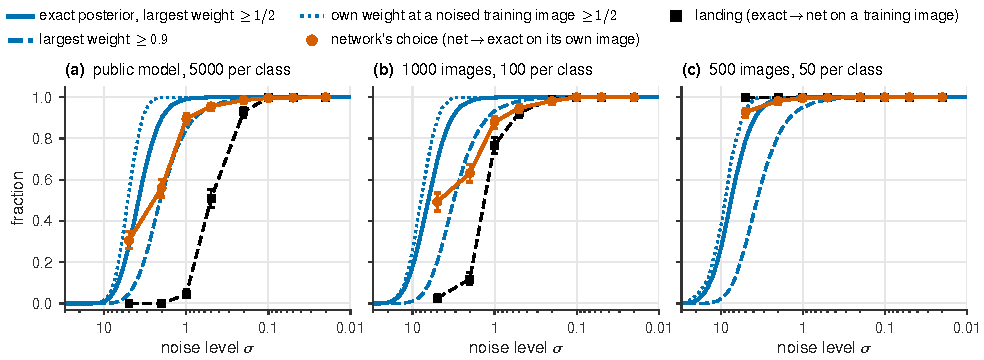
\includegraphics[width=\textwidth]{fig_posterior_choice.pdf}
\caption{Choice and landing against the concentration of the exact posterior (EDM on CIFAR-10;
sampling runs left to right). On the public model the network chooses its image where the exact
posterior at noised test images concentrates, and lands much later. The $1000$-image model makes
its last choices later than its range, and the memorising $500$-image model lands from every swap
level. Blue: the exact posterior over the training images of a class, share of noised test points
whose largest weight is at least $1/2$ (solid) or $0.9$ (dashed), and share of noised training
images whose weight on that image is at least $1/2$ (dotted), for the training set of each model.
Vermillion: share of net$\to$exact endpoints on the nearest training image of the network's own
endpoint ($=$L). Black: share of exact$\to$net endpoints on a training image. Eight swap levels $s$,
drawn at $\sigma=s$, $500$ latents per model, Wilson $95\%$ intervals. (a)~Public model;
(b)~$1000$ images, $0.5$\,Mimg; (c)~$500$ images.}
\label{fig:posterior}
\end{figure}

\paragraph{Window swaps.} \texttt{paperB\_window\_swap.py} samples the public model from the
$500$ latents of the swaps with the exact field at the levels $\sigma_k\in(\sigma_{\rm lo},
\sigma_{\rm hi}]$ of the schedule and the network at the others, for the windows of
Table~\ref{tab:window}; $(0,s]$ is net$\to$exact and $(s,\infty)$ exact$\to$net at level $s$. These
two kinds reproduce the endpoint images and shares of Table~\ref{tab:swap} exactly and its median
distances to within $0.001$. The two predictions of Section~\ref{sec:swap} were written down before
the run (the first restates the exact$\to$net runs of Table~\ref{tab:swap}): that the
median $d_1$ of exact$\to$net is $k\sigma_{\rm lo}$ with $k\in[20,35]$ and increases with
$\sigma_{\rm lo}$; and that for a window $(\sigma_{\rm lo},\sigma_{\rm hi}]$ the median $d_1$
changes by at most $20\%$ when $\sigma_{\rm hi}$ moves from $0.5$ to $2$. Intervals are Wilson
intervals for shares and, for ratios of medians, a bootstrap over latents stratified by class
($4000$ resamples, \texttt{paperB\_window\_analysis.py}).

\begin{table}[h]
\centering\small
\begin{tabular}{@{}lcccc@{}}
\toprule
exact field on & off-atom [$95\%$] & $=$L & $=$E & median $d_1$\\
\midrule
no level (network) & $1.000$ & $1.000$ & $0.138$ & $20.04$\\
every level & $0.000$ & $0.138$ & $1.000$ & $0.00$\\
\midrule
$(0,0.02]$ & $0.000$ & $1.000$ & $0.138$ & $0.00$\\
$(0,0.1]$ & $0.000$ & $0.996$ & $0.138$ & $0.00$\\
$(0,0.5]$ & $0.000$ & $0.956$ & $0.150$ & $0.00$\\
\midrule
$(0.02,\infty)$ & $0.000$ & $0.138$ & $1.000$ & $0.61$\\
$(0.05,\infty)$ & $0.000$ & $0.138$ & $1.000$ & $1.37$\\
$(0.1,\infty)$ & $0.002$ & $0.138$ & $1.000$ & $2.57$\\
$(0.2,\infty)$ & $0.070$ & $0.138$ & $1.000$ & $4.22$\\
$(0.5,\infty)$ & $0.492$ & $0.138$ & $1.000$ & $6.45$\\
$(1,\infty)$ & $0.956$ & $0.138$ & $1.000$ & $9.21$\\
\midrule
$(0.02,0.5]$ & $0.000$ & $0.956$ & $0.150$ & $0.78$\\
$(0.05,0.5]$ & $0.000$ & $0.956$ & $0.150$ & $1.93$\\
$(0.05,2]$ & $0.000$ & $0.560$ & $0.278$ & $1.33$\\
$(0.05,5]$ & $0.000$ & $0.306$ & $0.522$ & $1.33$\\
$(0.1,0.5]$ & $0.214$ $[0.180,0.252]$ & $0.956$ & $0.150$ & $4.16$\\
$(0.1,1]$ & $0.024$ $[0.014,0.041]$ & $0.896$ & $0.160$ & $3.04$\\
$(0.1,2]$ & $0.004$ $[0.001,0.014]$ & $0.560$ & $0.278$ & $2.48$\\
\bottomrule
\end{tabular}
\caption{Window swaps on the public model, $500$ latents. The exact field runs at the levels of
the $18$-step schedule in the window and the network at the others; $(0,s]$ is net$\to$exact and
$(s,\infty)$ exact$\to$net at level $s$, as in Table~\ref{tab:swap}. Columns as there; median
$d_1$: median distance of the endpoint to its nearest training image.}
\label{tab:window}
\end{table}

\begin{figure}[t]
\centering
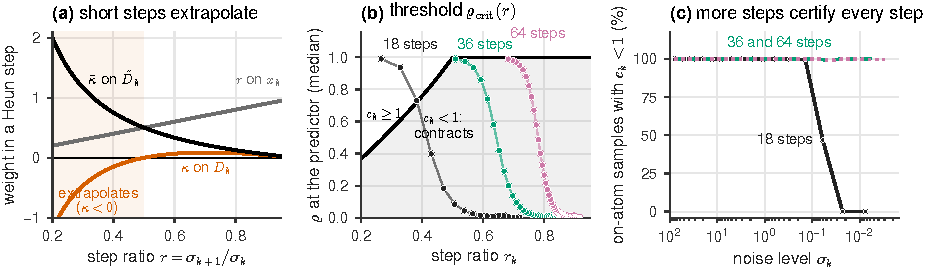
\includegraphics[width=\textwidth]{fig_heun.pdf}
\caption{Proposition~\ref{prop:heun} on EDM's schedule. (a) Weights of a Heun step against the step
ratio $r$; below $r=1/2$ the weight $\kappa$ on the first denoiser output is negative and the step
extrapolates. (b) The threshold $\varrho_{\rm crit}(r)$ (line; shaded: $c_k<1$) with the median
relative error at the Euler predictor of on-atom samples of the $500$-image model, one point per
step, joined in step order, for $18$, $36$ and $64$ steps. (c) Share of on-atom samples with
$c_k<1$ at each step: at least $99.6\%$ at every step with $36$ and $64$ steps, while with $18$
steps it falls to $47\%$ at $\sigma_k=0.060$ and to $0\%$ at the last two steps.}
\label{fig:heun}
\end{figure}

\paragraph{Heun bound along the trajectories.} Figure~\ref{fig:heun} and Table~\ref{tab:edm-heun} evaluate
Proposition~\ref{prop:heun}(b) with $\gamma=0$, $\varrho_k$ the larger of the relative errors at
$x_k$ and at $\tilde x_k$, and $\zeta$ from the exact posterior. The predictor's relative error is
the larger one at every step and every on-atom sample; it is close to the relative error at the
next level $\sigma_{k+1}$, where the predictor is evaluated. $\zeta/n$ is zero to working
precision at these steps, since the subset images are far apart.

\begin{table}[h]
\centering\small
\begin{tabular}{@{}rrrrrrrrrr@{}}
\toprule
step & $\sigma_k$ & $r_k$ & $\varrho_{\rm crit}$ & $\varrho$ at $x_k$ & $\varrho$ at $\tilde x_k$ & $c_k<1$ & factor & bound & public\\
\midrule
10 & 1.09 & 0.538 & 1 & 0.024 & 0.042 & $100\%$ & 0.540 & 0.549 & 0.600\\
11 & 0.585 & 0.506 & 1 & 0.043 & 0.085 & $100\%$ & 0.512 & 0.530 & 0.680\\
12 & 0.296 & 0.471 & 0.924 & 0.086 & 0.182 & $100\%$ & 0.485 & 0.535 & 0.829\\
13 & 0.140 & 0.430 & 0.825 & 0.185 & 0.397 & $99.7\%$ & 0.482 & 0.640 & 0.946\\
14 & 0.060 & 0.383 & 0.720 & 0.400 & 0.730 & $47\%$ & 0.581 & 1.011 & 0.989\\
15 & 0.023 & 0.328 & 0.608 & 0.725 & 0.937 & $0\%$ & 0.807 & 1.575 & 0.998\\
16 & 0.0075 & 0.266 & 0.487 & 0.929 & 0.990 & $0\%$ & 0.953 & 2.265 & 1.000\\
\bottomrule
\end{tabular}
\caption{Heun bound on the subset model, on-atom medians: factor $n_{k+1}/n_k$, bound
$(c_kn_k+b_k)/n_k$, and the factor of the public model. No step of any of the $1500$ trajectories
(both models) violates the bound.}
\label{tab:edm-heun}
\end{table}

\begin{table}[t]
\centering\small
\begin{tabular}{@{}rrrrrr@{}}
\toprule
Heun steps & $\min_kr_k$ & off-atom & certified at every step & violations & same image as $18$ steps\\
\midrule
18 & 0.266 & $4.1\%$ & $0\%$ & 0 & --\\
36 & 0.509 & $4.0\%$ & $99.5\%$ & 0 & $99.4\%$ / $94.8\%$\\
64 & 0.682 & $3.9\%$ & $99.5\%$ & 0 & $99.3\%$ / $94.4\%$\\
\bottomrule
\end{tabular}
\caption{Number of Heun steps, same latents. ``Certified'': on-atom samples of the subset model
with $c_k<1$ at every step. Last column: subset / public model.}
\label{tab:edm-steps}
\end{table}

\paragraph{Predictive anchor, baseline and thresholds.} Table~\ref{tab:edm-anchor} replaces the
endpoint's nearest image by the nearest training image of $D_\theta(x_k,\sigma_k)$, which uses no
information after $\sigma_k$, and compares with the distance $\hat d$ from $D_\theta$ to that image,
the baseline of the off-image test. Intervals are $95\%$ stratified bootstrap intervals ($1000$
resamples, paired for differences). The absolute error $e_t$ (from the separate run of
\texttt{n3\_edm\_memorization.py}, same model) is below the baseline at the same $\sigma$, by
$0.169$, $0.207$, $0.074$, $0.017$ and $0.004$ for the five columns, every interval excluding
zero. With off-atom thresholds $0.2$ and $0.5$ there are $46$ and $39$ off-atom samples, and every
AUC and the sign of every difference are unchanged.

\begin{table}[t]
\centering\footnotesize\setlength{\tabcolsep}{5pt}
\begin{tabular}{@{}lrrrrr@{}}
\toprule
$\sigma$ & 19.4 & 12.9 & 8.4 & 5.32 & 3.26\\
\midrule
anchor $=$ endpoint image (on-atom) & $0.496$ & $0.750$ & $0.901$ & $0.974$ & $0.994$\\
AUC of $\varrho$, endpoint anchor & $0.519$ & $0.670$ & $0.884$ & $0.974$ & $0.995$\\
AUC of $\varrho$, predictive anchor & $0.519$ & $0.670$ & $0.884$ & $0.974$ & $0.995$\\
AUC of the radial ratio & $0.796$ & $0.894$ & $0.946$ & $0.980$ & $0.996$\\
AUC of $\hat d$ (baseline) & $0.689$ & $0.876$ & $0.959$ & $0.991$ & $0.999$\\
radial ratio $-$ baseline & $0.106$ & $0.017$ & $-0.013$ & $-0.010$ & $-0.003$\\
\quad $95\%$ interval & $[0.056,0.159]$ & $[-0.009,0.043]$ & $[-0.027,0.001]$ & $[-0.017,-0.005]$ & $[-0.005,-0.001]$\\
\bottomrule
\end{tabular}
\caption{Predictive anchor and baseline, subset model ($1000$ samples, $41$ off-atom).}
\label{tab:edm-anchor}
\end{table}

\paragraph{Second seed and balanced model.} Table~\ref{tab:edm-models} repeats the main measurements
on all three trained models. The late contraction is
$C=\int_{0.002}^{0.585}(1-\varrho_\sigma)\,d\log(1/\sigma)$, computed with the trapezoidal rule on the
sampler's noise levels, and its AUC uses $-C$. The second $500$-image model reproduces the first. On
the $2000$-image model the relative error at a single noise level separates the groups less well
at the end ($0.929$ at $\sigma=0.002$), because on-atom samples also reach $\varrho\approx1$ there,
while the late contraction keeps an AUC of $0.983$. The baseline at $\sigma=0.002$ equals the
endpoint distance $d_1$ for every sample, since the last step of the sampler returns $D_\theta$ at
that level, so its AUC of $0.985$ is bookkeeping; at $\sigma=0.585$ the baseline has AUC $0.990$
(interval $[0.986,0.994]$), above the late contraction by $[0.004,0.010]$.

\begin{table}[t]
\centering\footnotesize
\begin{tabular}{@{}lrrrrrrrr@{}}
\toprule
model & off-atom & AUC $\varrho$, $\sigma=0.585$ & $0.140$ & $0.002$ & $C$ on / off & AUC of $C$ & baseline, $\sigma=0.585$ & $0.002$\\
\midrule
$500$ images, seed $0$ & $41$ & $1.000$ & $1.000$ & $0.995$ & $2.55$ / $0.29$ & $1.000$ & $1.000$ & $1.000$\\
$500$ images, seed $1$ & $44$ & $1.000$ & $1.000$ & $1.000$ & $2.53$ / $0.32$ & $1.000$ & $1.000$ & $1.000$\\
$2000$ images & $501$ & $0.990$ & $0.983$ & $0.929$ & $1.75$ / $0.68$ & $0.983$ & $0.990$ & $0.985$\\
\bottomrule
\end{tabular}
\caption{The three trained models, $1000$ samples each. $C$: late contraction (medians for on- and
off-atom samples). Baseline: AUC of the distance from $D_\theta$ to the nearest training image; at
$\sigma=0.002$ it equals the endpoint distance $d_1$, so that column is bookkeeping. The Heun bound
of Proposition~\ref{prop:heun} is never violated on any of them, and certifies every on-atom
sample down to $\sigma=0.30$ on all three.}
\label{tab:edm-models}
\end{table}

\paragraph{Worst-direction contraction.} On $200$ samples of the subset model ($13$ off-atom), the
median of $\mu=(1+\sigma)\lambda_{\max}$ of the symmetrised Jacobian of $D_\theta$ is $2.37$ off-atom
against $0.58$ on-atom at $\sigma=1.92$ (AUC $0.86$), but $0.96$ for both groups at
$\sigma\le0.023$ (AUC $0.52$ and $0.47$). The exact field has $\mu^\star=0$ there. Contraction in the
worst direction thus does not distinguish the groups late, while the radial ratio toward the
selected image, the quantity of Proposition~\ref{prop:trap} and the EDM form of Theorem~\ref{thm:relerr}(a), does, though at the last
steps partly by bookkeeping (Section~\ref{sec:contraction}).


% ==========================================================================
\section{Experimental details}
\label{app:expdetails}

A bracket after a five-seed EXP-1 mean (Section~\ref{sec:exp1}, Table~\ref{tab:exp1}) is a $95\%$ Student-$t$ interval for the mean, with four degrees of freedom
and a half-width of $1.39$ population standard deviations. A $\pm$ across seeds divides by $n$, not $n-1$; with five seeds,
the sample standard deviation would be about $12\%$ larger.

\subsection{Synthetic problems}
\label{app:exp}

\paragraph{EXP-1.} The prior is $x\sim\N(0,I_2)$, the observation is $y=Ax+\eta$ with a random
$1\times2$ matrix $A$ and $\eta\sim\N(0,0.1^2)$, and $N=200$ training pairs are drawn; the
posterior is Gaussian and analytic. The velocity network is a 4-layer, width-128 MLP with SiLU
activations and a 64-dimensional time embedding, trained with Adam (learning rate $10^{-3}$,
batch $256$) for $2\times10^5$ iterations without early stopping; label smoothing adds
$h\omega$ to the label at every step. Samples are generated with $100$ RK4 steps to
$t=1-10^{-3}$, $M=1000$ per condition, at $20$ training and $8$ held-out conditions. The seed fixes
both the problem instance and the training randomness. Before measurement, the analytic posterior
satisfies the normal equations to $1.8\times10^{-15}$ and closed-form integration of $(\star)$ maps
every $x_0$ to its atom. Table~\ref{tab:exp1} gives the hard-conditioning trajectory; the
runs at $h=0.1$ are used only for the measured transfer of Appendix~\ref{app:measured-transfer}. The memorisation ratio of
\citet{yoon2023memorization} is the fraction of samples whose nearest training point is at most
$\tfrac13$ as far as the second nearest; it starts from a common $\approx0.11$.

\begin{table}[htb]
\centering\footnotesize\setlength{\tabcolsep}{5pt}
\begin{tabular}{lccccc}
\toprule
& \multicolumn{5}{c}{iteration}\\
\cmidrule(l){2-6}
quantity & $10^2$ & $10^4$ & $10^5$ & $2\times10^5$ & $1\times10^6$ \\
\midrule
conditional $\tr\Cov$ & $1.08$\,[$1.04$, $1.11$] & $1.03$\,[$0.88$, $1.18$] & $0.58$\,[$0.33$, $0.83$] & $0.396$\,[$0.220$, $0.573$] & $0.120$\,[$0.046$, $0.195$]\\
velocity rel.\ error vs.\ ($\star$) & $0.78$\,[$0.73$, $0.83$] & $0.75$\,[$0.65$, $0.85$] & $0.50$\,[$0.44$, $0.55$] & $0.40$\,[$0.33$, $0.47$] & $0.168$\,[$0.095$, $0.241$]\\
$\|\text{mean}-x^i\|$ & $0.90$\,[$0.68$, $1.12$] & $0.87$\,[$0.59$, $1.16$] & $0.58$\,[$0.40$, $0.76$] & $0.38$\,[$0.24$, $0.52$] & $0.137$\,[$0.047$, $0.227$]\\
$\|\text{mean}-\mu_{\mathrm{post}}\|$ & $0.15$\,[$0.06$, $0.24$] & $0.25$\,[$0.15$, $0.35$] & $0.52$\,[$0.38$, $0.66$] & $0.66$\,[$0.41$, $0.90$] & $0.816$\,[$0.577$, $1.055$]\\
unconditional $\tr\Cov$ & $1.85$\,[$1.09$, $2.61$] & $1.93$\,[$1.72$, $2.15$] & $1.91$\,[$1.67$, $2.15$] & $1.926$\,[$1.690$, $2.163$] & ---\\
\bottomrule
\end{tabular}
\caption{EXP-1 at $h=0$, five seeds: mean and $95\%$ Student-$t$ interval for the mean (four
degrees of freedom). The $10^6$ column is a run with a cosine learning-rate schedule
($10^{-3}\to10^{-6}$) and no unconditional counterpart. Reference values:
$\tr\Sigmapost=1.018$ $[0.996,1.040]$ and $\tr\Xhat=1.931$ $[1.706,2.157]$, which the
unconditional row matches. Paired over seeds, $\tr\Cov/\tr\Sigmapost$ is $0.389$ $[0.217,0.560]$
at $2\times10^5$, the cosine run at $10^6$ lies $0.276$ $[0.160,0.393]$ below the constant-rate
run at $2\times10^5$ (a change of both schedule and length), and the unconditional
$\tr\Cov/\tr\Xhat$ is $0.997$ $[0.971,1.024]$.}
\label{tab:exp1}
\end{table}

% Table tab:p7kernel (EXP-1 label smoothing against the kernel reference) moved to paper A
% with kernel tracking (split contract, sec. 2).

\begin{figure}[htb]
\centering
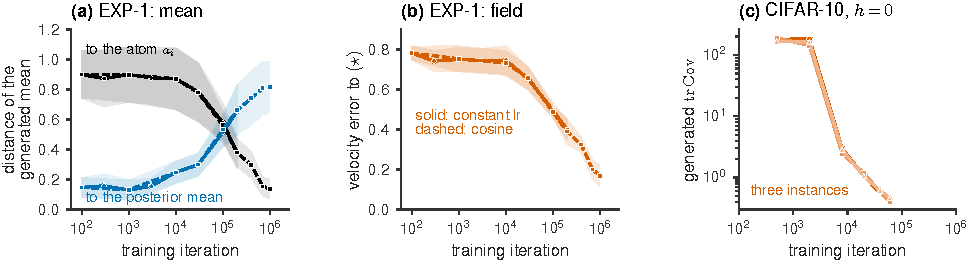
\includegraphics[width=\textwidth]{fig_collapse_details.pdf}
\caption{Further diagnostics for Figure~\ref{fig:collapse}. (a,~b)~EXP-1 at $h=0$, five seeds
(mean $\pm$ one population standard deviation; solid: constant learning rate, dashed: cosine
schedule to $10^6$ iterations): the generated mean leaves the posterior mean (blue) for the
training atom $x^i$ (black), and the learned velocity approaches the collapsed field $(\star)$ of
Proposition~\ref{prop:collapse}; values as in Table~\ref{tab:exp1}. (c)~The CIFAR-10 U-Net at
$h=0$: generated variance against iteration for the three independently redrawn instances
(training-time estimator, $8$ conditions, $M=16$).}
\label{fig:collapse-details}
\end{figure}

\paragraph{EXP-2 and EXP-3.} EXP-2 replaces the Gaussian prior by a bimodal mixture; mode
coverage is $1.0$ up to $\sim\!10^4$ iterations and then falls to $0.72$, while the share of samples
nearest the mode containing $x^i$ rises from $\approx0.5$ to $1.000$. EXP-3 is MNIST inpainting with
$N=500$ and a small U-Net, three seeds: the inpainted-region variance falls from
$0.137\pm0.021$ to $(1.17\pm0.12)\times10^{-3}$ by 15000 iterations, and the nearest-training-image
distance to $(0.77\pm0.26)\times10^{-3}$.

\paragraph{Architecture and optimiser.} Collapse does not depend on the network used.
Table~\ref{tab:ablation} varies the width and depth of the EXP-1 MLP and replaces Adam by SGD
(momentum $0.9$, learning rate $0.01$), with two seeds each and the same budget of $2\times10^5$
iterations. Every configuration falls well below $\tr\Sigmapost=1.018$; capacity and the
optimiser change the speed of the collapse, not its direction. Beyond the baseline, more capacity
lowers the training loss without a deeper collapse at this budget. Proposition~\ref{prop:collapse}
constrains the minimiser, not the model, so this is the expected pattern.

\begin{table}[htb]
\centering\small
\begin{tabular}{lcccc}
\toprule
configuration & width & depth & optimiser & $\tr\Cov$ at $2\times10^5$ \\
\midrule
baseline (5 seeds) & 128 & 4 & Adam & $0.396\pm0.127$\\
narrow & 32 & 4 & Adam & $0.657\pm0.041$\\
 & 64 & 4 & Adam & $0.526\pm0.041$\\
wide & 256 & 4 & Adam & $0.403\pm0.056$\\
shallow & 128 & 2 & Adam & $0.860\pm0.110$\\
deep & 128 & 6 & Adam & $0.407\pm0.090$\\
SGD & 128 & 4 & SGD & $0.711\pm0.136$\\
\bottomrule
\end{tabular}
\caption{EXP-1 at $h=0$, architecture and optimiser variants, two seeds each unless stated
(population standard deviations). The final training loss is $0.586$ for the baseline and $0.460$
for the width-$256$ network, whose variance is nevertheless the same.}
\label{tab:ablation}
\end{table}

\paragraph{Instance and training randomness.} The EXP-1 error bars vary one seed that fixes both
the problem instance (the operator $A$, hence $\Sigmapost$, and the training set) and the
training run. Two further sweeps of ten runs each separate them at $2\times10^5$ iterations.
With the instance fixed and the training seed varied, $\tr\Cov=0.338\pm0.064$; with the training
seed fixed and the instance varied, $0.404\pm0.121$ (population standard deviations). The
instance accounts for about $78\%$ of the combined variance. Every run collapses, with values
between $0.18$ and $0.57$; the two sweeps share the run with both seeds at $0$.

\subsection{CIFAR-10}
\label{app:exp4}

The network is the DDPM U-Net (base width 128, channel multipliers $(1,2,2,2)$, two residual
blocks per level, attention at resolution 16; $35.75$M parameters), trained with Adam (learning
rate $2\times10^{-4}$, batch 128, mixed precision) for $60000$ iterations on $N=2000$ training
images, conditioning on the top half ($k=1536$) and generating the bottom half. Bandwidths are
$h\in\{0,4,5,6\}$, against a nearest-neighbour median label distance of about $12.6$. Each
bandwidth is repeated on three independently redrawn instances, which vary the training subset
and the training randomness together. The final checkpoints of the first instance were re-measured
at $48$ conditions and $M=256$ samples per condition; only the $h=0$ trajectory quoted in the main
text uses the training-time estimator ($8$ conditions, $M=16$), whose final value $0.431$ compares
with $0.458$ re-measured. The networks of Appendix~\ref{app:measured-transfer} were retrained with
the same configuration at $h=4,5,6$.
Figure~\ref{fig:cifar-training-grid} shows the $h=0$ samples of the first instance through
training.

\begin{figure}[htb]
\centering
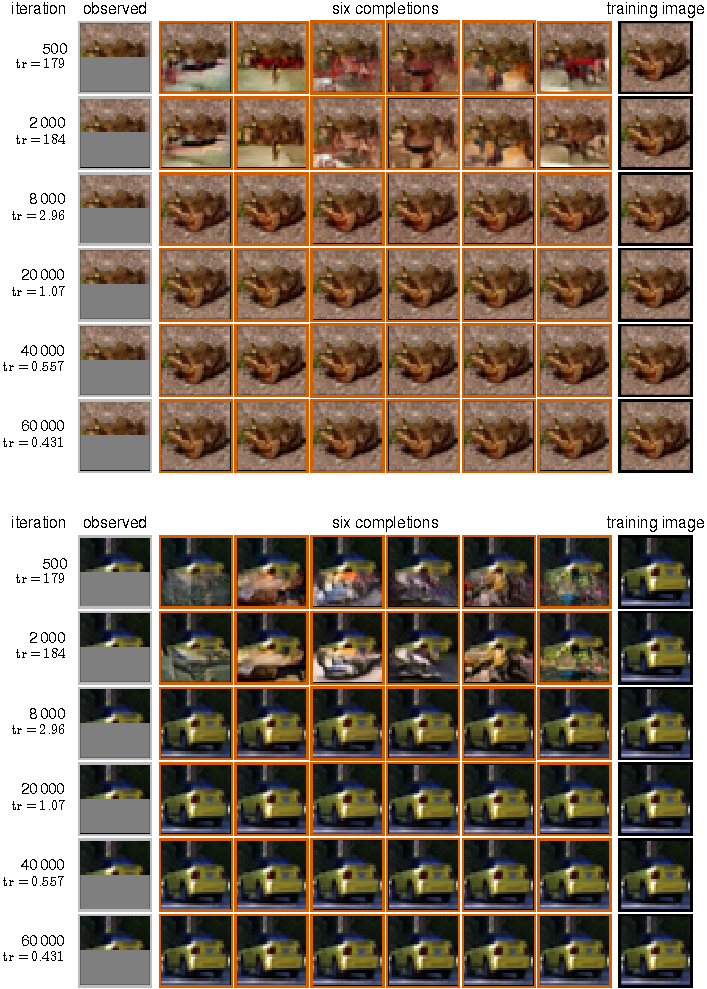
\includegraphics[width=0.78\textwidth]{fig_image_training.pdf}
\caption{CIFAR-10 U-Net at $h=0$, first instance: two conditions (top and bottom block) at iterations
$500$, $2000$, $8000$, $20000$, $40000$ and $60000$ (rows; under each iteration, the generated
trace from the training-time estimator). Each row shows the observed top half, six completions
from different sources $x_0$ and the training image. Early completions vary; from iteration
$8000$ all six reproduce the training image in both conditions.}
\label{fig:cifar-training-grid}
\end{figure}

\paragraph{Class labels.} With the CIFAR-10 class as the label, about $200$ of the $N=2000$
training images share each label, so Assumption~\ref{as:standing}(iii) fails. At $h=0$ the
posterior over atoms given a shared label is then the prior that is uniform on the images of
that class. The endpoint law of the exact flow for the empirical conditional law of the class
(cf.\ \citealp{baptista2025memorization}), with this prior in place of the uniform prior on all
atoms (cf.\ \citealp{wan2025elucidating}), gives the within-class empirical law as the exact endpoint law. Its
variance, the within-class scatter, is $717$ rather than $0$. Two runs of the same U-Net with the
one-hot class as the label, at $h=0$ and $h=0.4$, keep this variance
(Figure~\ref{fig:image-class}): the trace of the completions stays at $0.64$--$0.83$ of the
within-class scatter at $h=0$ and $0.62$--$1.30$ at $h=0.4$ over the six checkpoints, and both end
at $0.76$ while the training loss falls from $0.22$ to $0.06$. Shared labels therefore remove the
collapse onto one image; whether the completions stay on training images of the class is not
measured here.

\begin{figure}[htb]
\centering
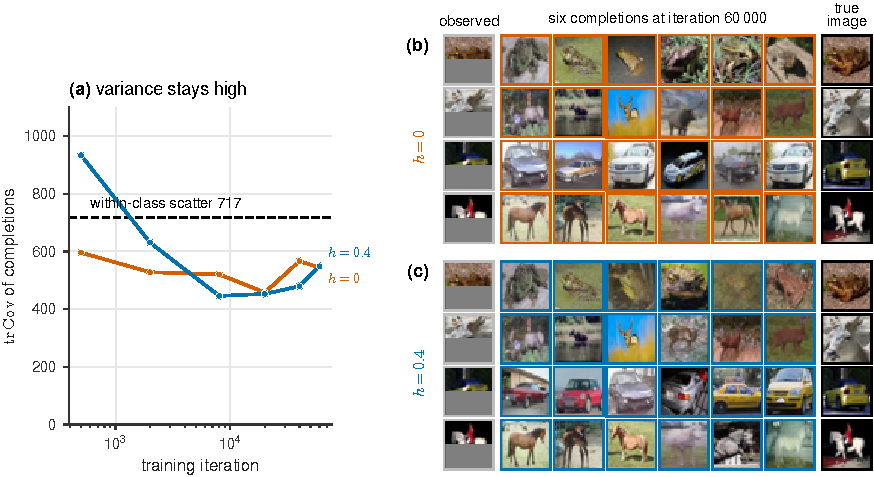
\includegraphics[width=\textwidth]{fig_image_class.pdf}
\caption{Class-conditional CIFAR-10 U-Net ($N=2000$, one seed). (a)~Trace of the covariance of
the completions, averaged over $10$ conditions, at the six checkpoints, against the within-class
scatter $717$ (dashed). (b,~c)~Completions of four conditions at iteration $60000$ for $h=0$ and
$h=0.4$: the observed top half, six completions from different sources $x_0$ and the true image. The model sees only the class, and its completions are
different images of that class.}
\label{fig:image-class}
\end{figure}

% Table tab:cifarddpm (CIFAR-10 variance against the kernel reference) moved to paper A with
% kernel tracking (split contract, sec. 2).

\end{document}
